% ---------------------------------------------------------------
% TCC2 - SENAC SANTO AMARO
% Texto do projeto do Matheus adaptado ao template atualizado do professor
% Tema: estudo comparativo multi-dataset em visão computacional (9 bases)
% ---------------------------------------------------------------

\documentclass[
    12pt,
    openright,
    oneside,
    a4paper,
    english,
    brazil
]{abntex2}

% ---------------------------------------------------------------
% PACOTES
% ---------------------------------------------------------------
\usepackage{lmodern}
\usepackage[T1]{fontenc}
\usepackage[utf8]{inputenc}
\usepackage{lastpage}
\usepackage{indentfirst}
\usepackage{color}
\usepackage{graphicx}
\graphicspath{{figuras/}}
\usepackage{microtype}
\usepackage{float}
\usepackage{booktabs}
\usepackage{multirow}
\usepackage{longtable}
\usepackage{amsmath,amssymb}
\usepackage{braket}
\usepackage{pgfgantt}
\usepackage[brazilian,hyperpageref]{backref}
\usepackage[alf]{abntex2cite}
\usepackage[
    left=3cm,
    right=2cm,
    top=3cm,
    bottom=2cm
]{geometry}

% ---------------------------------------------------------------
% CONFIGURAÇÕES DO PDF
% ---------------------------------------------------------------
\makeatletter
\hypersetup{
    pdftitle={\@title},
    pdfauthor={\@author},
    pdfsubject={TCC2 - SENAC Santo Amaro},
    pdfcreator={LaTeX with abnTeX2},
    pdfkeywords={tcc, senac, visão computacional, classificação de imagens, cnn, computação quântica, aprendizado de máquina quântico},
    colorlinks=true,
    linkcolor=blue,
    citecolor=blue,
    filecolor=magenta,
    urlcolor=blue,
    bookmarksdepth=4
}
\makeatother

\definecolor{blue}{RGB}{41,5,195}

% ---------------------------------------------------------------
% TAMANHO DA FONTE DAS LEGENDAS (TEMPLATE TCC2) -- 10 pt
% ---------------------------------------------------------------
\renewcommand{\ABNTEXfontereduzida}{\fontsize{10}{12}\selectfont}
\captionnamefont{\ABNTEXfontereduzida}
\captiontitlefont{\ABNTEXfontereduzida}
\makeatletter
\renewcommand{\legend}[1]{%
  \M@gettitle{#1}%
  \memlegendinfo{#1}%
  \par
  \begingroup
    \@parboxrestore
    \if@minipage
      \@setminipage
    \fi
    \ABNTEXfontereduzida
    \captiondelim{\mbox{}}%
    \@makecaption{}{\ignorespaces #1}\par
  \endgroup}
\makeatother

% ---------------------------------------------------------------
% INFORMAÇÕES DO DOCUMENTO
% ---------------------------------------------------------------
\titulo{Classificação de imagens em múltiplos benchmarks de visão computacional: um estudo comparativo entre CNNs clássicas e arquiteturas híbridas quântico-clássicas}
\autor{Matheus Sanchez Duda}
\local{São Paulo}
\data{2026}
\orientador{Prof. Jorge Echeimberg}
\coorientador{Prof. Thyago Quintas}

\instituicao{%
  SENAC -- Serviço Nacional de Aprendizagem Comercial
  \par
  Unidade Santo Amaro
  \par
  Bacharelado em Ciência da Computação
}

\tipotrabalho{Trabalho de Conclusão de Curso II}

\preambulo{Trabalho de Conclusão de Curso II apresentado ao SENAC Santo Amaro como requisito parcial para conclusão do curso de Ciência da Computação.}

\makeindex

\begin{document}
\selectlanguage{brazil}
\frenchspacing

% ---------------------------------------------------------------
% ELEMENTOS PRÉ-TEXTUAIS
% ---------------------------------------------------------------
\pretextual
\imprimircapa
\imprimirfolhaderosto

\begin{resumo}
Este trabalho tem como objetivo investigar e comparar de forma sistemática o desempenho de redes neurais convolucionais (CNNs) clássicas e arquiteturas híbridas quântico-clássicas aplicadas à tarefa de classificação supervisionada de imagens em nove conjuntos de dados públicos de visão computacional (MNIST, Fashion-MNIST, KMNIST, EMNIST Balanced, CIFAR-10, CIFAR-100 Coarse, SVHN, GTSRB e FER2013). A pesquisa combina revisão bibliográfica estruturada por conjunto de dados com uma campanha experimental controlada que avalia o comportamento preditivo e a eficiência computacional dos modelos frente a diferentes complexidades visuais, resoluções espaciais, números de canais e distribuições de classes, contemplando ainda análises de funções de ativação, tamanhos de lote (\textit{batch size}), estratégias de quantização e execução multiplataforma. Busca-se avaliar a capacidade de generalização do modelo clássico de referência, do controle vetorial com gargalo dimensional e da cabeça híbrida quântico-clássica simulada, viabilizando uma comparação empírica e auditável entre os dois paradigmas.

\vspace{\onelineskip}
\noindent
\textbf{Palavras-chave}: visão computacional. classificação de imagens. redes neurais convolucionais. computação quântica. aprendizado de máquina quântico. modelos híbridos quântico-clássicos.
\end{resumo}

\begin{resumo}[Abstract]
\begin{otherlanguage*}{english}
This work aims to systematically investigate and compare the performance of classical convolutional neural networks (CNNs) and hybrid quantum-classical architectures applied to supervised image classification across nine public computer vision datasets (MNIST, Fashion-MNIST, KMNIST, EMNIST Balanced, CIFAR-10, CIFAR-100 Coarse, SVHN, GTSRB, and FER2013). The research combines a dataset-oriented literature review with a controlled experimental campaign that evaluates the predictive behavior and computational efficiency of the models under different visual complexities, spatial resolutions, channel counts, and class distributions, while also encompassing analyses of activation functions, batch sizes, quantization strategies, and cross-platform execution. It seeks to assess the generalization capability of the classical baseline model, the classical bottleneck control, and the simulated variational quantum head, enabling an auditable empirical comparison between both paradigms.

\vspace{\onelineskip}
\noindent
\textbf{Keywords}: computer vision. image classification. convolutional neural networks. quantum computing. quantum machine learning. hybrid quantum-classical models.
\end{otherlanguage*}
\end{resumo}

% Listas exigidas pelo template atualizado. São geradas a partir dos
% elementos que já constam do texto do trabalho.
\pdfbookmark[0]{\listfigurename}{lof}
\listoffigures*
\cleardoublepage

\pdfbookmark[0]{\listtablename}{lot}
\listoftables*
\cleardoublepage

\pdfbookmark[0]{Lista de Abreviaturas e Siglas}{loas}
\chapter*{Lista de Abreviaturas e Siglas}
\begin{center}
\begin{tabular}{@{}p{3.2cm}p{0.6\textwidth}@{}}
\toprule
\textbf{Abreviatura/Sigla} & \textbf{Significado} \\
\midrule
AUC & \textit{Area Under the Curve} (Área sob a Curva) \\
CNN & \textit{Convolutional Neural Network} (Rede Neural Convolucional) \\
GPU & \textit{Graphics Processing Unit} (Unidade de Processamento Gráfico) \\
NISQ & \textit{Noisy Intermediate-Scale Quantum} \\
PQC & \textit{Parameterized Quantum Circuit} (Circuito Quântico Parametrizado) \\
QML & \textit{Quantum Machine Learning} (Aprendizado de Máquina Quântico) \\
QPU & \textit{Quantum Processing Unit} (Unidade de Processamento Quântico) \\
RGB & \textit{Red, Green, Blue} (Vermelho, Verde e Azul) \\
ROC & \textit{Receiver Operating Characteristic} \\
TCC & Trabalho de Conclusão de Curso \\
\bottomrule
\end{tabular}
\end{center}
\cleardoublepage

\pdfbookmark[0]{\contentsname}{toc}
\tableofcontents*
\cleardoublepage

% ---------------------------------------------------------------
% ELEMENTOS TEXTUAIS
% ---------------------------------------------------------------
\textual


% ---------------------------------------------------------------
% CAPÍTULO 1 - INTRODUÇÃO
% ---------------------------------------------------------------

\chapter{Introdução}

O avanço da Inteligência Artificial e do Aprendizado Profundo (\textit{Deep Learning}) consolidou novos padrões de desempenho em tarefas complexas de reconhecimento de padrões e visão computacional. Entre essas aplicações, a classificação supervisionada de imagens destaca-se como um problema fundamental, abrangendo desde o reconhecimento de caracteres manuscritos e símbolos tipográficos até a categorização de objetos naturais, sinais de trânsito e expressões faciais em condições variadas de iluminação e resolução.

As redes neurais convolucionais (CNNs) estabeleceram-se como uma das principais abordagens para tarefas visuais devido à sua capacidade de extrair representações hierárquicas diretamente a partir da estrutura espacial dos pixels. No entanto, o desempenho e o custo operacional dessas arquiteturas permanecem sensíveis a escolhas metodológicas e de engenharia, tais como a função de ativação empregada, o tamanho do lote de treinamento (\textit{batch size}), o grau de desbalanceamento entre classes, a aplicação de técnicas de quantização e as características de hardware do ambiente de execução.

Paralelamente, a computação quântica e o Aprendizado de Máquina Quântico (\textit{Quantum Machine Learning} -- QML) têm despertado crescente interesse científico como paradigmas emergentes de processamento da informação. Modelos híbridos quântico-clássicos propõem a integração entre extratores clássicos de características e circuitos quânticos parametrizados (PQCs), buscando explorar propriedades como superposição e emaranhamento em espaços de Hilbert de alta dimensão. Contudo, sua aplicação prática em problemas de visão computacional ainda enfrenta gargalos severos de simulação clássica, compressão dimensional, estabilidade de gradientes e escalabilidade em múltiplos domínios.

Diante desse cenário, este trabalho propõe um estudo experimental comparativo entre arquiteturas clássicas baseadas em redes neurais convolucionais e arquiteturas híbridas quântico-clássicas avaliadas sobre nove conjuntos de dados de visão computacional. A pesquisa investiga não apenas o desempenho preditivo global e por classe (Macro-F1, acurácia, precisão, revocação e matrizes de confusão), mas também a telemetria de treinamento, o impacto de hiperparâmetros e a viabilidade prática das abordagens em um protocolo experimental estritamente controlado e reprodutível.

Assim, este capítulo apresenta o contexto da pesquisa, a justificativa, os objetivos geral e específicos, a hipótese científica e as delimitações do trabalho.

\section{Contexto}

A classificação automática de imagens é um dos pilares da visão computacional moderna, servindo de base para sistemas autônomos, leitura óptica de documentos, inspeção industrial, segurança viária e interação humano-computador. Ao longo da última década, a disponibilidade de \textit{benchmarks} públicos padronizados permitiu avaliar a evolução de algoritmos sob diferentes níveis de dificuldade visual.

Conjuntos de dados em escala de cinza centrados em formas estruturadas --- como dígitos manuscritos (MNIST), caracteres cursivos japoneses Kuzushiji (KMNIST), letras e dígitos estendidos (EMNIST) e artigos de vestuário (Fashion-MNIST) --- oferecem cenários controlados para testar a capacidade de extração de contornos e topologias locais. Por outro lado, bases de imagens naturais e cenários reais --- como objetos cotidianos em baixa resolução (CIFAR-10 e CIFAR-100), dígitos em fachadas urbanas (SVHN), placas de trânsito sob variações climáticas e de perspectiva (GTSRB) e expressões faciais humanas (FER2013) --- impõem desafios substancialmente maiores, incluindo ruído de fundo, múltiplos canais de cor, variações de contraste e forte desbalanceamento entre categorias.

Nesse contexto, as redes neurais convolucionais destacam-se pela eficiência na extração automática de atributos espaciais por meio de filtros treináveis. Todavia, a busca por representações mais compactas e expressivas motivou a investigação de arquiteturas híbridas quântico-clássicas. Nesses modelos, camadas convolucionais clássicas atuam na redução da dimensionalidade espacial da imagem original para um vetor latente compacto, o qual é codificado em estados quânticos e processado por um circuito quântico variacional antes da camada de decisão final.

Entretanto, grande parte da literatura em Aprendizado de Máquina Quântico restringe seus experimentos a um único conjunto de dados simplificado --- frequentemente subconjuntos binários do MNIST ---, dificultando a compreensão de como essas arquiteturas se comportam quando submetidas a múltiplos domínios visuais, maior número de classes e variações sistemáticas de hiperparâmetros. Este trabalho insere-se exatamente nessa interseção entre visão computacional, engenharia de aprendizado profundo e aprendizado de máquina quântico, propondo um \textit{benchmark} consolidado em nove bases de dados para avaliar o comportamento real, os limites computacionais e a competitividade prática dos modelos clássicos e híbridos.

\section{Justificativa}

A justificativa deste trabalho estrutura-se em três dimensões complementares: tecnológica, acadêmica e metodológica.

Na dimensão tecnológica e prática, o treinamento e a inferência de modelos de visão computacional exigem um equilíbrio rigoroso entre qualidade preditiva (medida por métricas como Macro-F1) e eficiência computacional (tempo por época, \textit{throughput}, latência e consumo de memória de vídeo e sistema). Compreender como escolhas de funções de ativação, dimensionamento de lotes (\textit{batch sizes}), quantização pós-treinamento e arquiteturas de hardware (como estações Windows com GPUs dedicadas e sistemas Apple Silicon com memória unificada) afetam o desempenho em múltiplos domínios visuais fornece subsídios diretos para o projeto de sistemas eficientes de aprendizado de máquina.

Na dimensão acadêmica, embora o aprendizado profundo clássico esteja amplamente consolidado \cite{LeCun2015}, a integração de circuitos quânticos variacionais em \textit{pipelines} de visão computacional ainda carece de validação comparativa abrangente \cite{cerezo2021variational,long2025qcqcnn}. Investigar se a substituição ou complementação de camadas densas por cabeças híbridas quânticas traz ganhos ou perdas mensuráveis sob condições idênticas de pré-processamento contribui para separar expectativas teóricas da realidade experimental na era NISQ (\textit{Noisy Intermediate-Scale Quantum}).

Por fim, na dimensão metodológica e científica, observa-se uma lacuna importante na reprodutibilidade de estudos comparativos entre modelos clássicos e quânticos. Muitos trabalhos avaliam arquiteturas em cenários isolados, sem controle estrito de sementes aleatórias, sem varredura sistemática de hiperparâmetros e sem análise detalhada de resíduos e telemetria. Ao estabelecer uma campanha experimental padronizada sobre nove \textit{datasets} distintos, este TCC oferece uma base empírica sólida, auditável e reprodutível para a avaliação de modelos clássicos e híbridos.

\section{Objetivo geral}

Investigar e comparar sistematicamente o desempenho preditivo, a estabilidade de convergência e o custo computacional de redes neurais convolucionais (CNNs) clássicas e arquiteturas híbridas quântico-clássicas na classificação supervisionada de imagens ao longo de nove conjuntos de dados de visão computacional, avaliando o impacto de funções de ativação, tamanhos de lote, quantização e ambientes de execução.

\section{Objetivos específicos}

\begin{enumerate} 
    \item Estruturar e inventariar um conjunto padronizado de nove bases de dados públicas de visão computacional (MNIST, Fashion-MNIST, KMNIST, EMNIST Balanced, CIFAR-10, CIFAR-100 Coarse, SVHN, GTSRB e FER2013), caracterizando suas resoluções originais e efetivas, canais, variantes e distribuições de classes;
    \item Implementar um \textit{pipeline} experimental reprodutível de pré-processamento, divisão estratificada de dados, aumento de dados (\textit{data augmentation}) controlado, treinamento, validação e teste;
    \item Desenvolver e otimizar uma arquitetura de CNN clássica de referência, avaliando o impacto de diferentes funções de ativação, tamanhos de lote (\textit{batch sweep}) e estratégias de quantização;
    \item Projetar uma arquitetura híbrida quântico-clássica compatível com as restrições atuais de simulação de circuitos quânticos parametrizados;
    \item Investigar configurações do componente quântico, incluindo número de qubits, estratégia de codificação de atributos (\textit{embedding}), topologia do \textit{ansatz} variacional e integração com camadas clássicas;
    \item Comparar o desempenho dos modelos utilizando métricas globais e por classe, tais como acurácia, precisão, revocação (\textit{recall}), Macro-F1, curvas de validação e matrizes de confusão;
    \item Analisar a telemetria de execução, contemplando tempo por época, tempo acumulado de campanha, \textit{speedup} entre plataformas (Windows e macOS), \textit{throughput} e latência em cenários quantizados;
    \item Discutir criticamente a paridade de resultados, as vantagens, as limitações práticas e as condições de viabilidade das abordagens clássica e híbrida quântico-clássica em múltiplos domínios visuais.
\end{enumerate}

\section{Hipótese}

Parte-se da hipótese de que uma arquitetura híbrida quântico-clássica, utilizando circuitos quânticos parametrizados simulados como cabeça de classificação acoplada a um extrator convolucional clássico, pode alcançar convergência estável e desempenho competitivo (superior ao acaso e próximo ao \textit{baseline} clássico em bases de menor cardinalidade de classes) quando submetida a um protocolo experimental controlado, mantendo-se constantes as divisões de dados, o pré-processamento e os critérios de otimização.

Entretanto, não se pressupõe superioridade irrestrita da abordagem híbrida sobre as CNNs puramente clássicas. Considerando o gargalo de compressão dimensional exigido pelo número reduzido de qubits, o custo exponencial da simulação clássica de estados quânticos e a dificuldade de separação em problemas com dezenas de classes ou alta variabilidade intraclasse (como GTSRB, FER2013 e CIFAR-100), espera-se que a viabilidade prática dos modelos híbridos seja fortemente condicionada pela complexidade do \textit{dataset}, pelo dimensionamento do lote (\textit{batch size}) e pela eficiência do acoplamento entre a extração clássica e o circuito variacional.

\section{Delimitações do trabalho}

Este trabalho é delimitado como um estudo experimental comparativo em visão computacional e aprendizado de máquina. A tarefa investigada restringe-se à classificação supervisionada de imagens estáticas bidimensionais distribuídas em nove conjuntos de dados públicos de referência. Os experimentos com circuitos quânticos são conduzidos integralmente via simulação numérica em hardware clássico, não contemplando execução direta em processadores quânticos físicos (QPUs), de modo a isolar o comportamento algorítmico das arquiteturas das imperfeições de ruído físico de hardware externo e garantir total reprodutibilidade dos treinamentos.

% ---------------------------------------------------------------
% CAPÍTULO 2 - REVISÃO BIBLIOGRÁFICA
% ---------------------------------------------------------------
\chapter{Revisão Bibliográfica}

\section{Metodologia da pesquisa bibliográfica}

A revisão bibliográfica deste trabalho foi estruturada a partir da seguinte pergunta norteadora: \textit{quais arquiteturas clássicas e híbridas quântico-clássicas foram aplicadas à classificação supervisionada de imagens nas nove bases de dados do TCC, sob quais protocolos experimentais e com quais resultados preditivos e custos computacionais relatados?}

Para responder a essa questão de forma rastreável, a investigação bibliográfica foi organizada em duas frentes complementares:
\begin{enumerate}
    \item \textbf{Frente de fundamentação teórica e metodológica}: voltada às publicações originais que instituíram os conjuntos de dados do \textit{benchmark} \cite{lecun1998gradient,xiao2017fashionmnist,clanuwat2018kmnist,cohen2017emnist,krizhevsky2009learning,netzer2011svhn,stallkamp2012gtsrb,goodfellow2013fer2013}, aos fundamentos de processamento digital de imagens e aprendizado profundo \cite{gonzalez2008digital,LeCun2015,goodfellow2016deep,szegedy2014going,he2016resnet,huang2017densenet,deisenroth2020mathematics}, à explicabilidade espacial via Grad-CAM \cite{selvaraju2020gradcam}, às métricas de avaliação multiclasse e tratamento de desbalanceamento \cite{hand2001simple,fawcett2006roc,silva2025balanceamento} e às bases conceituais de computação quântica, circuitos variacionais e ferramentas de simulação \cite{nielsen2010quantum,biamonte2017qml,preskill2018nisq,mcclean2018barren,havlicek2019supervised,perezsalinas2020data,schuld2021effect,cerezo2021variational,faj2023warpspeed,bayraktar2023cuquantum,chen2024quantumhpcworkflow}. Nessa frente, admitiram-se obras anteriores ao recorte temporal recente sempre que constituíram fontes originais ou seminais indispensáveis;
    \item \textbf{Frente de estudos empíricos correlatos por conjunto de dados}: voltada à identificação de publicações que relatam resultados experimentais em pelo menos uma das nove bases selecionadas (MNIST, Fashion-MNIST, KMNIST, EMNIST Balanced, CIFAR-10, CIFAR-100 Coarse, SVHN, GTSRB e FER2013), exigindo descrição identificável da variante do \textit{dataset}, do número de classes, da arquitetura, do protocolo de avaliação e das métricas empregadas, distinguindo-se explicitamente artigos revisados por pares de pré-publicações (\textit{preprints}).
\end{enumerate}

É importante distinguir os parâmetros adotados nessas duas etapas para preservar a reprodutibilidade do relato. Na revisão narrativa de fundamentação e contextualização tecnológica, foram consultados trabalhos publicados predominantemente entre 2020 e 2026 (além das obras seminais anteriores), em português e inglês, utilizando termos combinados por operadores booleanos sobre visão computacional, redes neurais convolucionais, funções de ativação, dimensionamento de lotes (\textit{batch size}), quantização \cite{zandieh2025turboquant}, aprendizado de máquina quântico e circuitos variacionais \cite{egginger2024hyperparameter,ibmQuantumAerSimulation2026,qiskitMachineLearningTorchConnector2026}. Por sua vez, para o levantamento empírico direcionado aos nove conjuntos de dados do \textit{benchmark}, conduziu-se um mapeamento bibliográfico preliminar automatizado com recorte temporal principal de 2021 a 2026 e publicações em língua inglesa, complementado por verificação manual direta nas fontes primárias. Entre as consultas booleanas estruturadas por domínio e conjunto de dados destacam-se expressões como:
\begin{itemize}
    \item \texttt{("MNIST" OR "Fashion-MNIST") AND ("quantum neural network" OR "variational quantum circuit") AND "image classification"};
    \item \texttt{"CIFAR-100" AND ("coarse" OR "superclass") AND "image classification"};
    \item \texttt{"GTSRB" AND (CNN OR quantum) AND classification}.
\end{itemize}

No processamento preliminar automatizado das buscas orientadas às bases de dados, foram coletadas \textbf{5.925 ocorrências brutas}, as quais originaram \textbf{3.297 grupos distintos} após o agrupamento e remoção de duplicatas. Nessa etapa automatizada, \textbf{1.025 registros} foram sinalizados preliminarmente como candidatos aderentes e \textbf{2.272 registros} foram excluídos automaticamente. Cumpre ressaltar, como limitação metodológica explícita, que essas contagens refletem um \textbf{mapeamento bibliográfico preliminar}, e não o total imediato de artigos elegíveis: a triagem automatizada depende da disponibilidade de resumos nos metadados exportados (podendo descartar registros sem resumo completo) e não substitui a decisão humana de elegibilidade baseada na leitura integral do protocolo experimental. A partir desse mapeamento e da conferência focalizada por conjunto de dados, consolidou-se uma amostra de 28 registros levantados (19 clássicos e 9 quânticos/híbridos), acrescida de estudos candidatos verificados pontualmente para cobrir lacunas específicas das nove bases, cuja rastreabilidade individual encontra-se documentada no Apêndice~\ref{ap:matriz_revisao}. A Figura~\ref{fig:funil_busca_bibliografica} sintetiza as etapas desse fluxo de identificação, triagem e extração.

\begin{figure}[H]
    \centering
    \caption{Fluxo de busca, triagem preliminar e extração de dados da revisão bibliográfica.}
    \label{fig:funil_busca_bibliografica}
    \begin{tabular}{p{0.26\textwidth}p{0.64\textwidth}}
        \toprule
        \textbf{Etapa do fluxo} & \textbf{Procedimento e registro documental} \\
        \midrule
        1. Identificação e coleta & Levantamento de obras de fundamentação (2020--2026 e fontes seminais) e mapeamento preliminar por \textit{dataset} (2021--2026, inglês), totalizando 5.925 ocorrências brutas coletadas no funil automatizado. \\
        2. Agrupamento e desduplicação & Consolidação de versões redundantes e entradas repetidas entre consultas, resultando em 3.297 grupos únicos no mapeamento preliminar. \\
        3. Triagem preliminar & Filtragem inicial de título, resumo e palavras-chave (1.025 candidatos sinalizados automaticamente e 2.272 excluídos preliminarmente, sujeita à conferência humana). \\
        4. Verificação de elegibilidade & Conferência manual da fonte primária quanto à identificação do artigo, variante exata do \textit{dataset}, número de classes, partição avaliada (teste, validação ou treino), arquitetura e métrica reportada. \\
        5. Extração padronizada & Registro estruturado dos estudos clássicos e quântico-clássicos verificados na seção de trabalhos correlatos (Seção~\ref{sec:trabalhos_correlatos}) e na matriz de rastreabilidade (Apêndice~\ref{ap:matriz_revisao}). \\
        \bottomrule
    \end{tabular}
    \legend{Fonte: Elaborado pelo autor (2026).}
\end{figure}

Para a síntese comparativa dos estudos empíricos elegíveis, foram extraídos sistematicamente os seguintes campos: autor, ano e identificador digital (DOI); situação de citação e verificação no TCC; conjunto de dados e variante exata; quantidade de classes efetivamente avaliadas (distinguindo tarefas binárias, subconjuntos reduzidos e formulações multiclasse completas); volumes e origem das partições de treino, validação e teste; pré-processamento e aumento de dados; arquitetura neural clássica ou híbrida; otimizador, número de épocas, tamanho de lote (\textit{batch size}) e controle de sementes (\textit{seeds}) quando informados; partição à qual o resultado numérico se refere (teste, validação ou treino); métrica reportada (acurácia, Macro-F1 ou taxa de erro); tempos de execução e ambiente computacional; e limitações metodológicas ou inconsistências internas entre texto e tabelas originais. Especificamente para os modelos quânticos e híbridos, registraram-se ainda o número de qubits \textbf{por circuito}, a quantidade de circuitos acoplados, a estratégia de codificação (\textit{embedding}), a topologia do \textit{ansatz} variacional (ou o uso de filtro quântico fixo não treinável), a presença de modelo de ruído, o número de \textit{shots} e o emprego de simulador numérico ou processador quântico físico. Trabalhos binários, multiclasse e com diferentes divisões foram analisados segundo seus respectivos protocolos, sem presumir equivalência direta entre acurácias publicadas e o Macro-F1 obtido na campanha experimental deste TCC.

\section{Classificação de imagens e diversidade de domínios em visão computacional}

Esta seção apresenta os conceitos fundamentais relacionados aos diferentes domínios visuais abordados em \textit{benchmarks} de visão computacional. O objetivo é contextualizar as propriedades visuais, estruturais e estatísticas que diferenciam tarefas de reconhecimento de caracteres, objetos, sinais de trânsito e expressões faciais.

\subsection{Reconhecimento de dígitos, caracteres e símbolos manuscritos}

O reconhecimento óptico de caracteres e dígitos manuscritos constitui uma das aplicações precursoras da visão computacional e do aprendizado profundo \cite{LeCun2015}. Nesse domínio, as imagens são tipicamente adquiridas ou pré-processadas em escala de cinza (\(C=1\)), com o objeto de interesse centralizado sobre um fundo uniforme de baixo ruído. A informação discriminativa concentra-se na topologia dos traços, nas curvaturas, nas extremidades e nas interseções geométricas.

Enquanto dígitos arábicos ocidentais (como no conjunto MNIST) apresentam dez classes bem definidas e baixa ambiguidade estrutural, extensões alfanuméricas (como o EMNIST) e sistemas de escrita historicamente complexos --- a exemplo dos caracteres cursivos japoneses Kuzushiji no KMNIST --- introduzem variações caligráficas acentuadas, maior número de classes ou múltiplas formas visuais para representar um mesmo fonema ou conceito. Em cenários não controlados, como a leitura de números residenciais em cenas urbanas (SVHN), o reconhecimento de dígitos deixa de ocorrer sobre fundo limpo e passa a enfrentar variações severas de iluminação, fontes tipográficas diversas, desfoque de movimento e interferência de dígitos adjacentes.

\subsection{Categorização de artigos de vestuário, objetos naturais e sinalização viária}

À medida que a visão computacional avança de símbolos gráficos para objetos do mundo físico, a complexidade textural e espacial das imagens aumenta significativamente. No reconhecimento de artigos de vestuário em escala de cinza (como no Fashion-MNIST), embora a resolução espacial reduzida (\(28 \times 28\) pixels) seja idêntica à de bases de dígitos, os objetos apresentam silhuetas preenchidas, texturas internas sutis e forte similaridade interclasse (como entre camisas, camisetas, casacos e pulôveres).

Em imagens naturais coloridas (representadas no espaço RGB com \(C=3\) canais), como nos conjuntos CIFAR-10 e CIFAR-100, os modelos precisam distinguir categorias animais e veículos em resoluções compactas (\(32 \times 32\) pixels), nas quais o objeto de interesse convive com fundos complexos, oclusões parciais e variações de pose e escala. De forma análoga, o reconhecimento de placas de trânsito em ambientes reais (como no \textit{benchmark} GTSRB) exige que o classificador seja robusto a mudanças drásticas de iluminação diurna e noturna, intempéries climáticas, distorções de perspectiva e desbalanceamento acentuado entre categorias de sinalização frequentes e raras.

\subsection{Reconhecimento de expressões faciais e desafios de variabilidade intraclasse}

O reconhecimento automático de expressões faciais (como na base FER2013) representa um domínio particularmente desafiador dentro da classificação supervisionada de imagens. Diferentemente de objetos rígidos ou símbolos gráficos, a face humana sofre deformações não rígidas sutis nos músculos ao redor dos olhos, sobrancelhas e boca para expressar estados emocionais como raiva, desgosto, medo, felicidade, tristeza, surpresa e neutralidade.

Do ponto de vista computacional, esse domínio caracteriza-se por uma elevada variabilidade intraclasse --- pessoas de diferentes idades, etnias, gêneros e condições de iluminação expressam a mesma emoção de maneiras distintas --- combinada a uma baixa separabilidade interclasse, uma vez que expressões como medo e surpresa, ou tristeza e neutralidade, compartilham configurações geométricas muito próximas. Além disso, bases coletadas em condições não controladas (\textit{in-the-wild}) costumam apresentar rótulos ruidosos, oclusões por óculos ou mãos e forte assimetria na quantidade de exemplos por classe, exigindo arquiteturas com alta capacidade de regularização.

\section{Bases de dados e benchmarks utilizados no estudo}

A utilização de múltiplos conjuntos de dados públicos e padronizados é essencial para avaliar a capacidade de generalização, a estabilidade numérica e a escalabilidade de algoritmos de aprendizado de máquina. A adoção de um \textit{benchmark} multi-dataset evita que conclusões arquiteturais fiquem restritas às peculiaridades estatísticas de uma única fonte de dados, permitindo contrastar o desempenho de modelos clássicos e híbridos em diferentes regimes de resolução, dimensionalidade de canais e número de classes.

\subsection{Importância da avaliação multi-dataset em aprendizado profundo e quântico}

Na literatura de visão computacional, arquiteturas que apresentam excelente desempenho em bases simples de dígitos frequentemente sofrem degradação expressiva quando submetidas a imagens com texturas densas, múltiplos canais de cor ou dezenas de classes. No campo do Aprendizado de Máquina Quântico, essa questão é ainda mais crítica: como circuitos quânticos simulados operam com poucos qubits, a redução dimensional imposta pelo extrator clássico pode preservar informações suficientes para separar dez classes simples, mas colapsar representações em domínios mais complexos.

Por esse motivo, o protocolo experimental deste trabalho foi desenhado sobre um conjunto diversificado de nove bases de dados, documentadas e gerenciadas de forma centralizada no repositório do projeto (\path{configs/datasets.yaml} e \path{notebooks/dataset_inventory.ipynb}). Essa seleção abrange desde \textit{benchmarks} canônicos de validação rápida até problemas multiclasse com forte desbalanceamento e ruído visual.

\subsection{Caracterização dos 9 conjuntos de dados do benchmark}

Os nove conjuntos de dados adotados nos experimentos compreendem diferentes domínios de aplicação, resoluções nativas, quantidades de canais e números de classes, devendo-se distinguir suas especificações e divisões originais daquelas efetivamente aplicadas na campanha experimental auditada:

\begin{enumerate}
    \item \textbf{MNIST} (\textit{Modified National Institute of Standards and Technology}) \cite{lecun1998gradient}: Base clássica composta por 70.000 imagens em escala de cinza (\(28 \times 28 \times 1\)) de dígitos manuscritos de 0 a 9 (10 classes), dividida originalmente em 60.000 amostras de treino e 10.000 de teste. Na campanha experimental auditada, as partições de treino, validação e teste contaram com 48.999, 10.503 e 10.498 amostras, respectivamente.
    \item \textbf{Fashion-MNIST} \cite{xiao2017fashionmnist}: Proposta como substituição direta e mais desafiadora ao MNIST, contém 70.000 imagens em escala de cinza (\(28 \times 28 \times 1\)) distribuídas equilibradamente em 10 classes de artigos de vestuário (camiseta/top, calça, pulôver, vestido, casaco, sandália, camisa, tênis, bolsa e bota), com 49.000 amostras de treino, 10.500 de validação e 10.500 de teste na campanha auditada.
    \item \textbf{KMNIST} (\textit{Kuzushiji-MNIST}) \cite{clanuwat2018kmnist}: Composta por 70.000 imagens em escala de cinza (\(28 \times 28 \times 1\)) distribuídas em 10 classes de caracteres cursivos japoneses (Hiragana clássico), apresentando topologias de traços significativamente mais complexas e maior variação intraclasse do que os dígitos arábicos, dividida na campanha auditada em 49.000 imagens de treino, 10.500 de validação e 10.500 de teste.
    \item \textbf{EMNIST Balanced} (\textit{Extended MNIST -- Balanced}) \cite{cohen2017emnist}: Variante balanceada da extensão alfanumérica do conjunto NIST contendo \textbf{47 classes} de caracteres manuscritos (dígitos e letras maiúsculas/minúsculas com fusão de classes visualmente indistinguíveis) em resolução nativa de \(28 \times 28 \times 1\) em escala de cinza, totalizando 131.600 imagens (divisão original padrão de 112.800 para treino e 18.800 para teste). Na campanha auditada, utilizaram-se 92.120 imagens de treino, 19.740 de validação e 19.740 de teste.
    \item \textbf{CIFAR-10} \cite{krizhevsky2009learning}: Conjunto de 60.000 imagens naturais coloridas em formato RGB (\(32 \times 32 \times 3\)), sendo originalmente 50.000 para treinamento e 10.000 para teste, divididas igualmente em 10 classes de objetos e animais (avião, automóvel, pássaro, gato, cervo, cachorro, sapo, cavalo, navio e caminhão). Na campanha auditada, a divisão foi de 42.000 amostras de treino, 9.000 de validação e 9.000 de teste.
    \item \textbf{CIFAR-100 Coarse} \cite{krizhevsky2009learning}: Possui a mesma estrutura física e volume total do CIFAR-10 (60.000 imagens RGB de resolução nativa \(32 \times 32 \times 3\)). Embora o conjunto original forneça também rótulos finos para 100 categorias, o recorte experimental adotado neste trabalho utiliza os rótulos de \textbf{20 superclasses (\textit{coarse})} oficiais, agrupando cinco classes finas em cada superclasse (3.000 imagens por superclasse), com partições auditadas de 42.000 imagens de treino, 9.000 de validação e 9.000 de teste.
    \item \textbf{SVHN} (\textit{Street View House Numbers}) \cite{netzer2011svhn}: Base de imagens reais obtidas a partir de fachadas residenciais no Google Street View, contendo dígitos recortados e centralizados em resolução nativa \(32 \times 32 \times 3\) (RGB) distribuídos em 10 classes (dígitos de 0 a 9). Suas divisões usuais compreendem 73.257 imagens de treino e 26.032 de teste (além de um conjunto extra separado). Na campanha auditada, foram empregadas 69.502 amostras de treino, 14.894 de validação e 14.893 de teste.
    \item \textbf{GTSRB} (\textit{German Traffic Sign Recognition Benchmark}) \cite{stallkamp2012gtsrb}: Conjunto composto por imagens RGB de placas de trânsito alemãs reais capturadas sob variadas condições de iluminação e distância, com tamanhos originais variáveis e distribuição fortemente desigual ao longo de 43 classes. Na campanha auditada, foram registradas 27.489 imagens de treino, 5.905 de validação e 5.876 de teste.
    \item \textbf{FER2013} (\textit{Facial Expression Recognition 2013}) \cite{goodfellow2013fer2013}: Base composta por 35.887 imagens faciais em escala de cinza de resolução nativa \(48 \times 48 \times 1\), distribuídas de maneira desbalanceada em 7 classes de expressões emocionais básicas (raiva, desgosto, medo, felicidade, tristeza, surpresa e neutro), com partições auditadas de 25.121 amostras de treino, 5.384 de validação e 5.382 de teste.
\end{enumerate}

A Tabela~\ref{tab:caracterizacao_9_datasets} sintetiza as dimensões nativas, o número de classes, o volume original e as divisões de treino, validação e teste efetivamente registradas na campanha experimental auditada em 30/10/2026. Cumpre destacar que, no pré-processamento dessa campanha auditada, as imagens foram redimensionadas tipicamente para \(64 \times 64\) pixels e, no caso do GTSRB, para \(128 \times 128\) pixels, e que as contagens da última coluna correspondem às partições geradas no experimento, não devendo ser confundidas com as divisões oficiais originais de cada \textit{benchmark}.

\begin{table}[htb]
\centering
\caption{Caracterização estrutural original e partições da campanha auditada para os 9 conjuntos de dados do \textit{benchmark}.}
\label{tab:caracterizacao_9_datasets}
\resizebox{\textwidth}{!}{%
\begin{tabular}{p{3.8cm}p{6.5cm}r}
\toprule
\textbf{Dataset e função} & \textbf{Imagens e classes originais} & \textbf{Treino / validação / teste na campanha auditada} \\
\midrule
\textbf{MNIST} \cite{lecun1998gradient} --- dígitos manuscritos & \(28 \times 28\), cinza; 10 classes; 70.000 imagens & 48.999 / 10.503 / 10.498 \\
\textbf{Fashion-MNIST} \cite{xiao2017fashionmnist} --- categorias de vestuário & \(28 \times 28\), cinza; 10 classes; 70.000 imagens & 49.000 / 10.500 / 10.500 \\
\textbf{KMNIST} \cite{clanuwat2018kmnist} --- caracteres japoneses Kuzushiji & \(28 \times 28\), cinza; 10 classes; 70.000 imagens & 49.000 / 10.500 / 10.500 \\
\textbf{EMNIST Balanced} \cite{cohen2017emnist} --- caracteres alfanuméricos & \(28 \times 28\), cinza; \textbf{47 classes}; 131.600 imagens (divisão padrão: 112.800/18.800) & 92.120 / 19.740 / 19.740 \\
\textbf{CIFAR-10} \cite{krizhevsky2009learning} --- objetos e animais & \(32 \times 32\), RGB; 10 classes; 60.000 imagens & 42.000 / 9.000 / 9.000 \\
\textbf{CIFAR-100 Coarse} \cite{krizhevsky2009learning} --- superclasses de objetos & \(32 \times 32\), RGB; \textbf{20 superclasses} (5 classes finas em cada uma); 60.000 imagens (fornece também 100 rótulos finos) & 42.000 / 9.000 / 9.000 \\
\textbf{SVHN} \cite{netzer2011svhn} --- dígitos de fachadas reais & \(32 \times 32\), RGB; 10 classes; divisões usuais de 73.257 treino e 26.032 teste (além de conjunto extra) & 69.502 / 14.894 / 14.893 \\
\textbf{GTSRB} \cite{stallkamp2012gtsrb} --- placas de trânsito & RGB, tamanhos originais variáveis; 43 classes e distribuição desigual & 27.489 / 5.905 / 5.876 \\
\textbf{FER2013} \cite{goodfellow2013fer2013} --- expressões faciais & \(48 \times 48\), cinza; 7 classes; 35.887 imagens e desbalanceamento & 25.121 / 5.384 / 5.382 \\
\bottomrule
\end{tabular}%
}
\legend{Fonte: Elaborado pelo autor (2026), com base nas fontes originais das bases e no relatório de auditoria experimental de 30/10/2026. Na campanha auditada, aplicou-se redimensionamento para \(64 \times 64\) pixels (e \(128 \times 128\) pixels no GTSRB).}
\end{table}

\textbf{Ressalva metodológica sobre o particionamento do GTSRB:} a auditoria experimental de 30/10/2026 identificou que, na partição utilizada para o GTSRB, pelo menos 3.990 das 5.876 imagens do subconjunto de teste possuíam outras imagens provenientes da mesma sequência física de captura (\textit{track}) alocadas no conjunto de treinamento. Uma vez que quadros sucessivos de uma mesma placa apresentam forte correlação visual, essa sobreposição entre \textit{tracks} facilita o acerto no subconjunto avaliado e restringe inferências sobre a generalização para sequências inteiramente novas. Por conseguinte, os resultados obtidos nessa base não devem ser denominados como desempenho no conjunto de teste oficial do \textit{benchmark}, registrando-se a separação estrita por sequência (\textit{track-aware split}) como requisito metodológico para novas campanhas de treinamento.

\subsection{Qualidade dos rótulos, desbalanceamento e heterogeneidade entre domínios}
\label{subsec:qualidade_rotulos_balanceamento_vies}

A análise conjunta das nove bases de dados evidencia desafios metodológicos distintos que justificam um protocolo rigoroso de avaliação. Em tarefas de classificação supervisionada, o desbalanceamento de classes --- fortemente presente em bases reais como SVHN, GTSRB e FER2013 --- tende a enviesar o gradiente de otimização em direção às classes majoritárias, reduzindo a sensibilidade do modelo para categorias minoritárias.

Segundo \citeonline{silva2025balanceamento}, estratégias de mitigação desse efeito podem atuar tanto em nível de dados (amostragem estratificada, \textit{oversampling}, \textit{undersampling} e aumento de dados direcionado) quanto em nível algorítmico (ponderação na função de perda e uso de métricas insensíveis à prevalência global). Além do desbalanceamento, a heterogeneidade entre domínios --- alternando entre imagens monocromáticas de \(28 \times 28\) ou \(48 \times 48\) pixels e imagens RGB de \(32 \times 32\) pixels --- exige que o \textit{pipeline} de avaliação reporte sistematicamente métricas agregadas de forma igualitária entre classes, como o Macro-F1, acompanhadas das matrizes de confusão e dos resíduos de desempenho por classe, garantindo uma comparação justa entre as arquiteturas clássica e híbrida.

\subsection{Tratamento do desbalanceamento de classes}
\label{subsec:tratamento_desbalanceamento_classes}

O tratamento do desbalanceamento de classes constitui um ponto metodológico central em tarefas de classificação supervisionada de imagens quando se avaliam \textit{benchmarks} coletados em cenários reais. Enquanto conjuntos curados em laboratório (como MNIST, Fashion-MNIST, KMNIST, CIFAR-10 e CIFAR-100) possuem quantidades uniformes ou quase uniformes de amostras por categoria, bases como GTSRB (43 classes de placas de trânsito), FER2013 (7 expressões faciais, com escassez acentuada na classe desgosto) e SVHN (predomínio dos dígitos ``1'' e ``2'') apresentam distribuições fortementes assimétricas. Quando essa distribuição é muito desigual, o modelo tende a favorecer as classes majoritárias, obtendo acurácia global aparentemente elevada, mas baixo desempenho justamente nas categorias menos representadas.

De forma geral, uma base de dados multiclasse pode ser representada por categorias \(C_0, C_1, \ldots, C_{K-1}\), cada uma contendo \(n_k\) amostras. O desbalanceamento ocorre quando:

\[
n_i \gg n_j
\quad \text{para determinadas classes } i \text{ e } j.
\]

Nesse cenário, a função de perda média calculada ao longo dos lotes de treinamento passa a ser dominada pelas classes com maior volume amostral, pois seus exemplos contribuem com maior frequência para a atualização dos gradientes. Assim, o objetivo das estratégias de controle de desbalanceamento não é distorcer a condição real do problema nos subconjuntos de avaliação, mas tornar o processo de aprendizagem e a análise de desempenho menos enviesados.

\citeonline{silva2025balanceamento} discute técnicas de equilíbrio de classes e destaca que métodos de balanceamento modificam a distribuição efetiva de treinamento, influenciando tanto a fronteira de decisão aprendida pelos classificadores quanto propriedades estatísticas do modelo. Por esse motivo, qualquer estratégia de reamostragem ou ponderação deve ser tratada como uma decisão metodológica explícita e controlada.

No nível de dados, destacam-se duas abordagens clássicas: o \textit{oversampling}, que amplia a presença das classes minoritárias no conjunto de treinamento (por repetição controlada de amostras ou por aumento de dados via transformações visuais que preservem o rótulo semântico), e o \textit{undersampling}, que reduz a quantidade de exemplos das classes majoritárias. A Figura~\ref{fig:balanceamento_over_under_silva2025} apresenta visualmente essas duas estratégias: o \textit{oversampling} preserva todas as amostras originais, mas pode elevar o custo por época e o risco de sobreajuste caso haja repetição excessiva sem diversidade; já o \textit{undersampling} reduz o tempo de treinamento e o domínio da classe majoritária, mas pode descartar exemplos informativos necessários para a generalização.

\begin{figure}[H]
    \centering
    \caption{Representação visual das estratégias de \textit{oversampling} e \textit{undersampling} no tratamento de classes desbalanceadas.}
    \label{fig:balanceamento_over_under_silva2025}
    \begin{minipage}{0.48\textwidth}
        \centering
        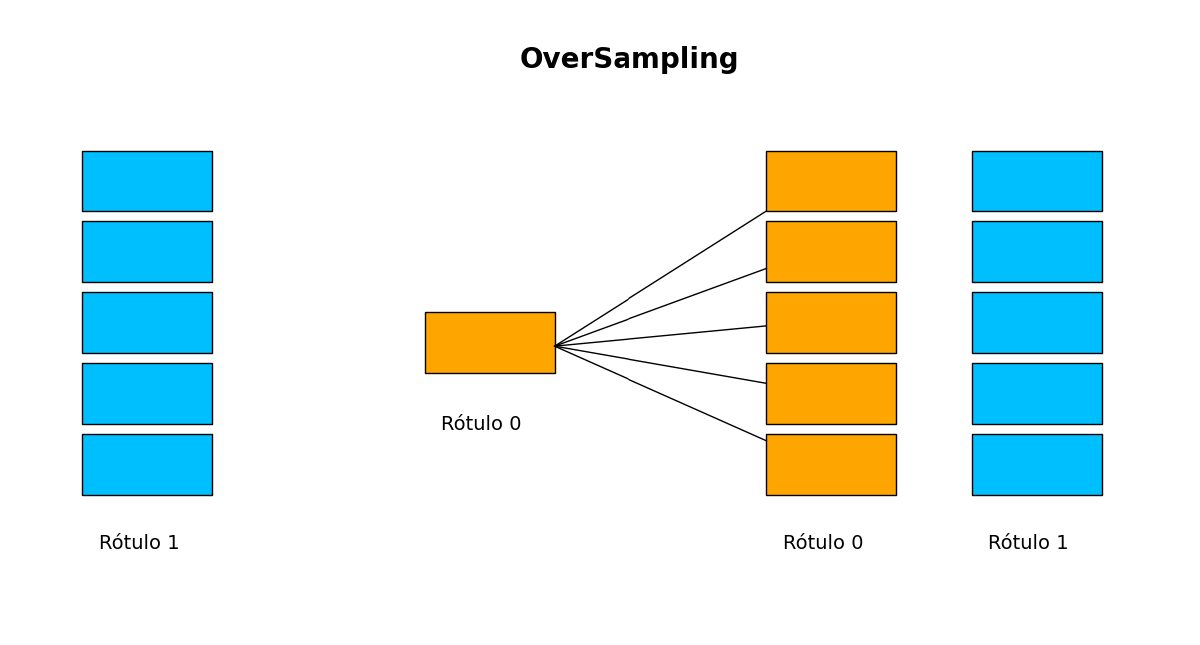
\includegraphics[width=\textwidth]{balanceamento_oversampling_silva2025.png}
    \end{minipage}
    \hfill
    \begin{minipage}{0.48\textwidth}
        \centering
        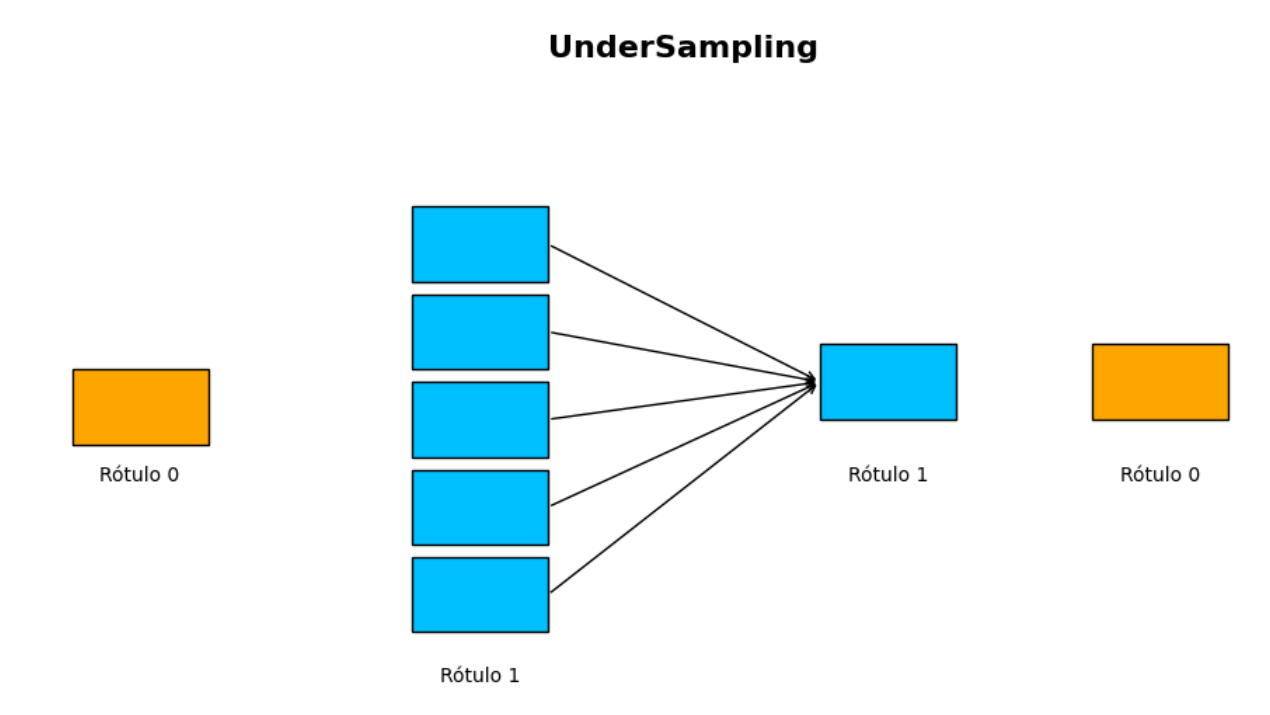
\includegraphics[width=\textwidth]{balanceamento_undersampling_silva2025.png}
    \end{minipage}
    \legend{Fonte: adaptado de \citeonline{silva2025balanceamento}.}
\end{figure}

Além das técnicas em nível de dados, destaca-se o aprendizado sensível a custos (\textit{cost-sensitive learning}) em nível algorítmico. Nessa abordagem, a distribuição amostral não é alterada diretamente, mas a função de perda passa a atribuir pesos diferenciados aos erros cometidos nas classes menos frequentes:

\[
\mathcal{L}_{custo} =
\frac{1}{N}
\sum_{i=1}^{N}
w_{y_i}\mathcal{L}(y_i, f_{\theta}(x_i)),
\]

em que \(w_{y_i}\) representa o peso associado à classe verdadeira \(y_i\) da amostra \(x_i\) (tipicamente inversamente proporcional à frequência \(n_{y_i}\)). Independentemente do uso de reamostragem ou ponderação no treinamento, um princípio metodológico inegociável adotado neste trabalho é que os conjuntos de validação e teste mantêm estritamente a distribuição original estratificada de cada uma das nove bases de dados, sendo avaliados prioritariamente pelo Macro-F1 e pela análise de resíduos por classe (\(\Delta\text{F1}\)).

\section{Imagens digitais e classificação computacional}

A classificação computacional de imagens depende da representação de informações visuais em estruturas numéricas manipuláveis por algoritmos. Em processamento digital de imagens, uma imagem pode ser formalmente descrita como uma função bidimensional discreta, composta por elementos finitos denominados pixels, cada um associado a uma posição espacial e a um ou mais valores de intensidade \cite{gonzalez2008digital}. Em \textit{benchmarks} de visão computacional, essa representação é fundamental, pois variações locais de intensidade, bordas, textura e contraste de cor determinam os padrões geométricos que diferenciam as classes de interesse. As redes neurais convolucionais consolidaram-se como a abordagem padrão para esse tipo de problema porque exploram diretamente a organização espacial das imagens por meio de filtros convolucionais aprendidos durante o treinamento, preservando relações de vizinhança entre pixels \cite{LeCun2015}.

\subsection{Representação computacional de imagens digitais}

Uma imagem digital pode ser compreendida matematicamente como uma função bidimensional discreta, geralmente representada por \(I(x,y)\), em que \(x\) e \(y\) indicam as coordenadas espaciais do pixel e \(I(x,y)\) representa o valor de intensidade naquele ponto da imagem. Em uma imagem em escala de cinza, como ocorre em bases monocromáticas de caracteres, artigos de vestuário e faces, cada pixel possui apenas um valor numérico associado à luminosidade local. Assim, uma imagem monocromática com altura \(H\) e largura \(W\) pode ser representada como uma matriz:

\[
I \in \mathbb{R}^{H \times W}
\]

A Figura~\ref{fig:imagem_matriz_5x5} apresenta uma representação simplificada dessa estrutura matricial. No exemplo, a imagem em escala de cinza é ampliada como uma grade \(5 \times 5\), na qual cada célula corresponde a um pixel. Ao lado, a mesma imagem é representada por uma matriz de intensidades, em que valores maiores indicam regiões mais claras e valores menores indicam regiões mais escuras.

\begin{figure}[H]
    \centering
    \caption{Representação matemática de uma imagem em escala de cinza como matriz de intensidades.}
    \label{fig:imagem_matriz_5x5}
    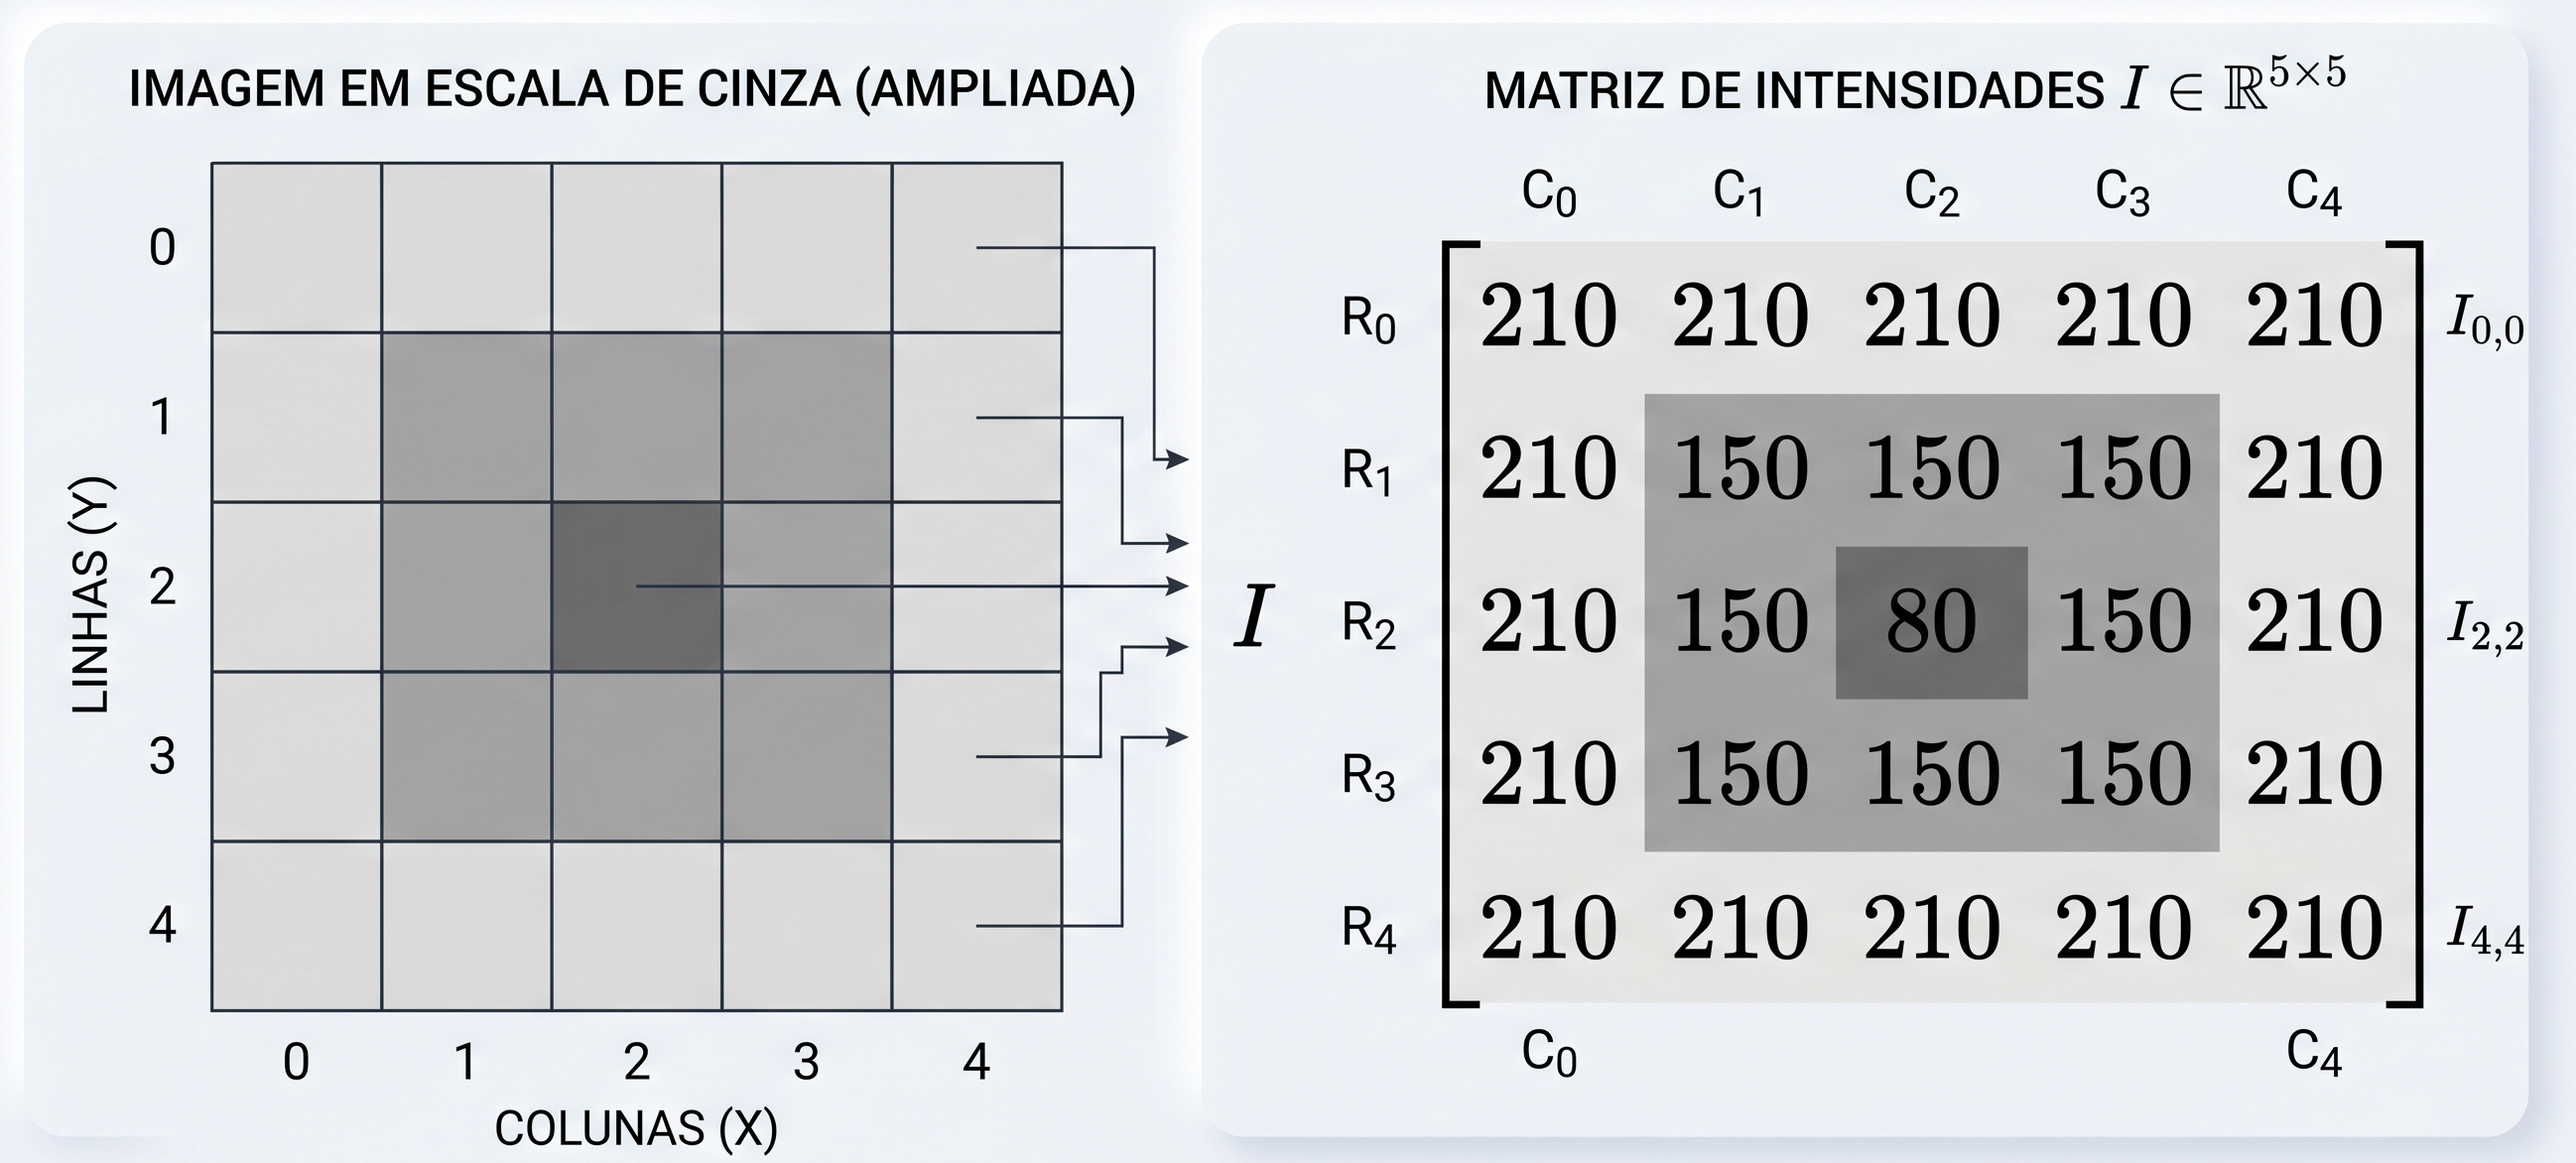
\includegraphics[width=\textwidth]{imagem_matriz_5x5.png}
    \legend{Fonte: Elaborado pelo autor (2026).}
\end{figure}

Em termos matemáticos, cada elemento \(I_{i,j}\) corresponde ao valor de intensidade do pixel localizado na linha \(i\) e na coluna \(j\). Em imagens de 8 bits, por exemplo, esses valores normalmente variam entre 0 e 255, sendo 0 associado ao preto, 255 ao branco e os valores intermediários aos diferentes tons de cinza. Em problemas de visão computacional, essa variação espacial de intensidade codifica contornos, gradientes de iluminação, texturas superficiais e estruturas morfológicas essenciais para discriminar o objeto de interesse.

Antes de ser utilizada por um modelo de aprendizado profundo, a imagem costuma passar por uma etapa de normalização. Uma forma simples de normalização consiste em dividir cada valor de pixel por 255, transformando a escala original para o intervalo entre 0 e 1:

\[
I'_{i,j} = \frac{I_{i,j}}{255}
\]

Essa transformação não altera a estrutura espacial da imagem, mas facilita o treinamento da rede neural, pois reduz a variação numérica dos dados de entrada. Em termos computacionais, uma imagem digital é representada de forma geral como um tensor de três dimensões:

\[
I \in \mathbb{R}^{H \times W \times C}
\]

em que \(H\) representa a altura, \(W\) a largura e \(C\) o número de canais de cor. Em bases monocromáticas (escala de cinza), como MNIST, Fashion-MNIST, KMNIST, EMNIST (\(28 \times 28 \times 1\)) e FER2013 (\(48 \times 48 \times 1\)), tem-se \(C = 1\). Já em bases de imagens coloridas no espaço RGB, como CIFAR-10, CIFAR-100, SVHN e GTSRB (\(32 \times 32 \times 3\)), tem-se \(C = 3\). Quando várias imagens são processadas simultaneamente durante o treinamento ou inferência, organiza-se um lote (\textit{batch}) de imagens representado pelo tensor de quarta ordem:

\[
X \in \mathbb{R}^{N \times H \times W \times C}
\]

em que \(N\) indica o tamanho do lote (\textit{batch size}, como \(N \in \{32, 64, 128, 256\}\)).

No contexto da classificação supervisionada multiclasse, cada imagem \(x\) é associada a um rótulo discreto \(y \in \{0, 1, \dots, K-1\}\), em que \(K\) representa o número total de classes do conjunto de dados (por exemplo, \(K=7\) no FER2013, \(K=10\) no MNIST, Fashion-MNIST, KMNIST, CIFAR-10 e SVHN, \(K=20\) no CIFAR-100 Coarse, \(K=43\) no GTSRB e \(K=47\) no EMNIST Balanced). O objetivo do modelo computacional é aprender uma função \(f_{\theta}(x)\), parametrizada por pesos treináveis \(\theta\), capaz de receber o tensor da imagem como entrada e produzir uma distribuição de probabilidade sobre as \(K\) classes possíveis:

\[
f_{\theta}(x) = [p_0, p_1, \dots, p_{K-1}]
\]

sendo a classe final prevista obtida pela regra de decisão de máxima probabilidade a posteriori:

\[
\hat{y} = \arg\max_{k \in \{0, \dots, K-1\}} p_k
\]

Essa formulação mostra que a classificação computacional de imagens não ocorre diretamente sobre a imagem visual percebida por um ser humano, mas sobre uma representação numérica estruturada. A imagem é convertida em matriz ou tensor, seus valores são normalizados, os rótulos são codificados numericamente e o modelo aprende padrões estatísticos capazes de relacionar regiões da imagem às classes de interesse.

Nas redes neurais convolucionais, esse processo é realizado por meio de filtros ou núcleos convolucionais que percorrem a imagem extraindo padrões locais. Um filtro \(K\) de tamanho \(m \times n\) é aplicado sobre pequenas regiões da imagem, produzindo novos mapas de características. De forma simplificada, a operação convolucional pode ser representada por:

\[
S(i,j) = \sum_{u=0}^{m-1}\sum_{v=0}^{n-1} K(u,v) \cdot I(i+u,j+v)
\]

Nesse caso, o filtro funciona como uma janela que analisa regiões locais da imagem. Dependendo dos valores aprendidos pelo filtro durante o treinamento, ele pode se tornar sensível a bordas, texturas, variações de contraste, formas ou padrões mais complexos. Em \textit{benchmarks} de visão computacional, essa propriedade é fundamental porque elementos discriminativos --- como traços caligráficos em caracteres, contornos de objetos naturais, pictogramas em placas de trânsito ou curvaturas faciais --- dependem diretamente das relações locais entre pixels vizinhos.

Portanto, a representação computacional de imagens digitais estabelece a ponte entre o sinal visual bruto e os modelos de aprendizado profundo e híbridos quântico-clássicos, permitindo que informações visuais de múltiplos domínios sejam transformadas em tensores numéricos processáveis.

\subsection{Classificação supervisionada de imagens}
\label{subsec:classificacao_supervisionada_imagens}

A classificação supervisionada de imagens é uma tarefa de aprendizado de máquina na qual um modelo aprende a associar imagens de entrada a rótulos previamente definidos. Diferentemente de abordagens não supervisionadas, nas quais o algoritmo busca padrões sem classes conhecidas, no aprendizado supervisionado cada amostra do conjunto de dados possui uma saída esperada, também chamada de rótulo ou \textit{ground truth}. Em \textit{benchmarks} de visão computacional, esses rótulos representam as categorias semânticas de cada domínio, como dígitos, caracteres, peças de vestuário, objetos naturais, sinais viários ou expressões faciais.

Do ponto de vista matemático, um conjunto de dados supervisionado pode ser representado por:

\[
\mathcal{D} =
\{(x_1,y_1),(x_2,y_2),\ldots,(x_N,y_N)\},
\]

em que \(x_i\) representa a \(i\)-ésima imagem e \(y_i\) representa seu respectivo rótulo. Em uma tarefa de classificação com \(K\) classes, cada rótulo pertence ao conjunto:

\[
y_i \in \{0,1,\ldots,K-1\}.
\]

Assim, a cardinalidade \(K\) adapta-se diretamente à granularidade semântica da base avaliada, abrangendo desde problemas com \(K=7\) ou \(K=10\) categorias até cenários com dezenas de classes (\(K=20\) superclasses no CIFAR-100 Coarse, \(K=43\) no GTSRB e \(K=47\) no EMNIST Balanced).

Segundo \citeonline{deisenroth2020mathematics}, a aprendizagem de máquina pode ser compreendida a partir de três componentes principais: dados, modelo e aprendizagem. Os dados precisam ser representados numericamente; o modelo é uma função parametrizada; e a aprendizagem corresponde ao ajuste dos parâmetros desse modelo com base nos exemplos disponíveis. No caso de imagens digitais, cada amostra é descrita como um tensor:

\[
x_i \in \mathbb{R}^{H \times W \times C},
\]

em que \(H\) representa a altura, \(W\) representa a largura e \(C\) representa o número de canais (\(C=1\) em imagens em escala de cinza e \(C=3\) em imagens coloridas RGB). Dessa forma, a imagem passa a ser uma estrutura matemática processável por algoritmos de otimização.

O objetivo de um modelo supervisionado é aprender uma função parametrizada capaz de mapear a entrada \(x_i\) para uma saída associada às \(K\) classes possíveis:

\[
f_{\theta}: \mathbb{R}^{H \times W \times C} \rightarrow \mathbb{R}^{K},
\]

em que \(\theta\) representa o conjunto de parâmetros aprendidos pelo modelo. Em redes neurais, esses parâmetros correspondem aos pesos e vieses das camadas (e, em modelos híbridos, incluem os ângulos de rotação das portas quânticas parametrizadas). A saída da rede geralmente é um vetor de escores (\textit{logits}), convertido em probabilidades por meio da função \textit{softmax}:

\[
p_k =
\frac{e^{s_k}}
{\sum_{j=0}^{K-1} e^{s_j}},
\]

em que \(s_k\) é o escore associado à classe \(k\), e \(p_k\) representa a probabilidade estimada para essa classe. A classe prevista pelo modelo é dada por:

\[
\hat{y} =
\arg\max_k p_k.
\]

Assim, o modelo atribui à imagem a classe que possui maior probabilidade estimada. Por exemplo, em uma tarefa ilustrativa com três classes, se a saída do modelo para uma amostra for:

\[
\hat{p} = [0{,}12,\ 0{,}23,\ 0{,}65],
\]

então a classe prevista será a terceira classe (\(k=2\)), pois \(0{,}65\) é o maior valor do vetor de probabilidades.

Durante o treinamento, a predição do modelo é comparada com o rótulo verdadeiro por meio de uma função de perda. Em problemas multiclasse, uma função amplamente utilizada é a entropia cruzada categórica (\textit{categorical cross-entropy}):

\[
\mathcal{L}(y,\hat{p}) =
-\sum_{k=0}^{K-1}
y_k \log(p_k),
\]

em que \(y_k\) representa o rótulo verdadeiro em codificação \textit{one-hot}. Quando a classe correta é \(c\), essa expressão pode ser simplificada para:

\[
\mathcal{L}(y,\hat{p}) =
-\log(p_c).
\]

Portanto, a perda será baixa quando o modelo atribuir alta probabilidade à classe correta e será alta quando o modelo atribuir baixa probabilidade ao rótulo verdadeiro. O treinamento consiste em ajustar os parâmetros \(\theta\) para minimizar essa perda ao longo do conjunto de dados, processo diretamente relacionado à otimização matemática em aprendizado de máquina \cite{deisenroth2020mathematics,goodfellow2016deep}.

Em \textit{benchmarks} de visão computacional com diferentes níveis de balanceamento e ruído visual, a classificação supervisionada exige cuidados metodológicos específicos. Bases coletadas em cenários reais (como SVHN, GTSRB e FER2013) apresentam variações acentuadas de iluminação, contraste, resolução nativa e distribuição entre classes, além de possíveis ambiguidades de rotulagem. Essas características tornam indispensável a padronização do pré-processamento, da divisão estratificada dos dados e das métricas de avaliação para assegurar comparações justas entre arquiteturas distintas.

\subsection{Treinamento, validação, teste e generalização}
\label{subsec:treinamento_validacao_teste_generalizacao}

Em aprendizado supervisionado, a avaliação adequada de um modelo depende da separação do conjunto de dados em subconjuntos com funções distintas. De modo geral, os dados são divididos em treino, validação e teste. O conjunto de treino é utilizado para ajustar os parâmetros do modelo; o conjunto de validação auxilia no acompanhamento do desempenho e na escolha de hiperparâmetros; e o conjunto de teste é reservado para estimar o desempenho final em dados não vistos.

Essa divisão é essencial porque o objetivo de um modelo de aprendizado de máquina não é apenas memorizar os exemplos usados no treinamento, mas generalizar para novas amostras. \citeonline{deisenroth2020mathematics} ressaltam que o aprendizado deve buscar desempenho em dados ainda não observados, e não apenas bom ajuste aos dados disponíveis. Em estudos multi-dataset, essa questão é central, pois uma configuração arquitetural ou de hiperparâmetros pode convergir rapidamente em bases canônicas de dígitos e apresentar degradação severa de generalização em imagens naturais ou expressões faciais.

Durante o treinamento, o modelo recebe os exemplos do conjunto de treino e atualiza seus parâmetros com base no erro calculado. Considerando uma função de perda \(\mathcal{L}\), o treinamento pode ser descrito pela minimização do risco empírico:

\[
R_{\text{emp}}(\theta)
=
\frac{1}{N}
\sum_{i=1}^{N}
\mathcal{L}(y_i, f_{\theta}(x_i)).
\]

O risco empírico mede o erro médio do modelo sobre os dados disponíveis para treinamento. No entanto, o interesse real está no desempenho esperado em dados novos. A diferença entre o erro de treino e o erro em validação ou teste está relacionada à capacidade de generalização do modelo.

A atualização dos parâmetros pode ser representada, de forma simplificada, por uma etapa de gradiente descendente:

\[
\theta_{t+1}
=
\theta_t
-
\eta
\nabla_{\theta}
R_{\text{emp}}(\theta_t),
\]

em que \(\theta_t\) representa os parâmetros na iteração \(t\), \(\eta\) é a taxa de aprendizado e \(\nabla_{\theta}R_{\text{emp}}(\theta_t)\) é o gradiente da função de perda em relação aos parâmetros. Esse processo é repetido ao longo de várias épocas, até que o modelo alcance um desempenho adequado ou até que critérios de parada sejam satisfeitos.

O conjunto de validação é utilizado para acompanhar o comportamento do modelo durante o treinamento. Ele permite verificar se a redução da perda no treino está acompanhada de melhora em dados não utilizados diretamente na atualização dos pesos. Além disso, a validação auxilia na escolha de hiperparâmetros, como taxa de aprendizado, função de ativação, tamanho do lote (\textit{batch size}), número de épocas, intensidade de regularização e estratégia de aumento de dados.

O conjunto de teste, por sua vez, deve ser utilizado somente ao final do processo de desenvolvimento. Sua função é fornecer uma estimativa imparcial do desempenho final do modelo. Caso o conjunto de teste seja usado repetidamente para tomar decisões de modelagem, ele deixa de representar uma avaliação independente, pois passa a influenciar indiretamente o ajuste do modelo.

A generalização pode ser compreendida como a capacidade do modelo de manter desempenho satisfatório em exemplos que não participaram do treinamento. Quando o modelo apresenta baixo erro no treino, mas erro elevado na validação ou no teste, ocorre o fenômeno conhecido como \textit{overfitting}, ou sobreajuste. Nesse caso, o modelo aprende detalhes específicos do conjunto de treino, como ruídos de fundo, artefatos de compressão ou particularidades amostrais, em vez de aprender padrões gerais associados às classes.

O comportamento típico do sobreajuste pode ser representado por:

\[
\mathcal{L}_{train} \downarrow
\quad \text{e} \quad
\mathcal{L}_{val} \uparrow,
\]

ou seja, a perda de treino continua diminuindo enquanto a perda de validação aumenta ou deixa de melhorar. Também pode ocorrer quando a métrica de desempenho no treino cresce continuamente, mas na validação se estabiliza ou diminui. \citeonline{goodfellow2016deep} discutem esse problema como uma das principais limitações de modelos de alta capacidade, especialmente quando a quantidade de exemplos por classe é reduzida (como no CIFAR-100 ou nas classes minoritárias do GTSRB e FER2013).

O fenômeno oposto é o \textit{underfitting}, ou subajuste. Ele ocorre quando o modelo não consegue aprender adequadamente nem mesmo os padrões presentes no conjunto de treino. Nesse caso, tanto o desempenho no treino quanto o desempenho na validação permanecem baixos. O subajuste pode ocorrer quando a arquitetura possui baixa capacidade representacional, quando há compressão excessiva de características (como em gargalos quânticos muito estreitos) ou quando o regime de otimização é insuficiente.

Outro cuidado metodológico indispensável é a prevenção de vazamento de dados (\textit{data leakage}) e a adoção de divisão estratificada entre treino, validação e teste. Em bases desbalanceadas, a partição estratificada preserva a proporção original das \(K\) classes em todos os subconjuntos, garantindo que categorias minoritárias estejam adequadamente representadas tanto durante o ajuste dos parâmetros quanto na avaliação final.

\subsection{Métricas de avaliação}
\label{subsec:metricas_avaliacao}

A avaliação de modelos de classificação em visão computacional deve ser compreendida a partir da formulação matemática geral do aprendizado supervisionado. Nesse contexto, considera-se um conjunto de dados composto por pares de entrada e rótulo:

\[
\mathcal{D} = \{(x_1,y_1),(x_2,y_2),\ldots,(x_N,y_N)\},
\]

em que \(x_i\) representa uma imagem de entrada e \(y_i \in \{0, 1, \dots, K-1\}\) representa seu rótulo verdadeiro entre as \(K\) classes do conjunto de dados avaliado.

Segundo \citeonline{deisenroth2020mathematics}, em uma tarefa de classificação multiclasse, o modelo pode ser representado por uma função parametrizada:

\[
f_{\theta}: \mathbb{R}^{D} \rightarrow \mathbb{R}^{K},
\]

em que \(D\) representa a dimensão da entrada após sua representação numérica, \(K\) representa o número de classes e \(\theta\) representa o conjunto de parâmetros do modelo. Para uma imagem \(x_i\), o modelo produz um vetor de probabilidades via \textit{softmax}:

\[
\hat{p}_i = f_{\theta}(x_i) = [p_{i,0}, p_{i,1}, \ldots, p_{i,K-1}],
\]

em que \(p_{i,k}\) representa a probabilidade estimada de a imagem \(x_i\) pertencer à classe \(k\), e a classe prevista é obtida por:

\[
\hat{y}_i = \arg\max_{k} p_{i,k}.
\]

Durante o treinamento, minimiza-se o risco empírico:

\[
R_{\text{emp}}(f_{\theta}) =
\frac{1}{N}
\sum_{i=1}^{N}
\ell(y_i, f_{\theta}(x_i)),
\]

utilizando-se tipicamente a entropia cruzada categórica:

\[
\mathcal{L}(y_i, \hat{p}_i) =
-\sum_{k=0}^{K-1} y_{i,k}\log(p_{i,k}),
\]

que para a classe verdadeira \(c\) se reduz a \(\mathcal{L}(y_i, \hat{p}_i) = -\log(p_{i,c})\). Entretanto, a função de perda utilizada na otimização contínua não é suficiente para caracterizar de forma completa a qualidade discriminativa do classificador nas \(K\) classes. Por isso, são utilizadas métricas de avaliação discretas e probabilísticas calculadas sobre os conjuntos de validação e teste.

A métrica mais direta é a acurácia, que mede a proporção de classificações corretas em relação ao total de amostras avaliadas:

\[
Accuracy =
\frac{1}{N}
\sum_{i=1}^{N}
\mathbb{1}(\hat{y}_i = y_i),
\]

em que \(\mathbb{1}(\hat{y}_i = y_i)\) é uma função indicadora que assume valor 1 quando a predição está correta e 0 caso contrário. Embora seja uma métrica intuitiva, a acurácia global pode ser enganosa em bases desbalanceadas, nas quais um classificador obtém valores elevados apenas por favorecer as categorias mais frequentes.

Para uma análise detalhada por categoria, utiliza-se a matriz de confusão. Em um problema com \(K\) classes, a matriz de confusão é definida por:

\[
C \in \mathbb{N}^{K \times K},
\]

em que cada elemento \(C_{ij}\) indica a quantidade de exemplos cuja classe verdadeira é \(i\) e cuja classe prevista é \(j\). De forma ilustrativa, para \(K=3\), tem-se:

\[
C =
\begin{bmatrix}
C_{00} & C_{01} & C_{02} \\
C_{10} & C_{11} & C_{12} \\
C_{20} & C_{21} & C_{22}
\end{bmatrix}.
\]

Os elementos da diagonal principal \(C_{kk}\) contabilizam os acertos do modelo para cada classe \(k\), enquanto os elementos fora da diagonal \(C_{ij}\) (\(i \neq j\)) revelam confusões semânticas ou morfológicas específicas de cada base (como a confusão entre camisa e camiseta no Fashion-MNIST, entre expressões faciais próximas no FER2013 ou entre caracteres cursivos semelhantes no KMNIST).

A partir da matriz de confusão, é possível calcular métricas específicas por classe usando a estratégia \textit{one-vs-rest}. Nessa abordagem, para cada classe \(k\), considera-se essa classe como positiva e todas as demais como negativas. Assim, definem-se:

\[
TP_k = C_{kk},
\]

\[
FN_k =
\sum_{\substack{j=0 \\ j \neq k}}^{K-1}
C_{kj},
\]

\[
FP_k =
\sum_{\substack{i=0 \\ i \neq k}}^{K-1}
C_{ik},
\]

\[
TN_k =
\sum_{\substack{i=0 \\ i \neq k}}^{K-1}
\sum_{\substack{j=0 \\ j \neq k}}^{K-1}
C_{ij}.
\]

Nessas expressões, \(TP_k\) representa os verdadeiros positivos da classe \(k\), isto é, exemplos da classe \(k\) corretamente classificados como \(k\). \(FN_k\) representa os falsos negativos, ou seja, exemplos da classe \(k\) classificados como outra classe. \(FP_k\) representa os falsos positivos, isto é, exemplos de outras classes classificados incorretamente como \(k\). Por fim, \(TN_k\) representa os verdadeiros negativos, ou seja, exemplos que não pertencem à classe \(k\) e também não foram classificados como \(k\).

A precisão da classe \(k\) é definida por:

\[
Precision_k =
\frac{TP_k}{TP_k + FP_k}.
\]

Essa métrica indica, entre todas as imagens classificadas pelo modelo como pertencentes à classe \(k\), quantas realmente pertencem a essa classe. Uma baixa precisão para determinada categoria indica que o modelo atribui excessivamente esse rótulo a amostras de outras classes, elevando a taxa de falsos positivos.

A revocação (\textit{recall}) ou sensibilidade é definida por:

\[
Recall_k = Sensitivity_k =
\frac{TP_k}{TP_k + FN_k}.
\]

Essa métrica indica a proporção de exemplos reais da classe \(k\) que foram corretamente identificados pelo modelo. Em classes minoritárias (como sinais de trânsito raros no GTSRB ou a expressão de desgosto no FER2013), uma baixa revocação evidencia que o modelo falha em detectar aquela categoria, gerando muitos falsos negativos.

A especificidade mede a capacidade do modelo de reconhecer corretamente os exemplos que não pertencem à classe analisada:

\[
Specificity_k =
\frac{TN_k}{TN_k + FP_k}.
\]

O F1-score combina precisão e revocação por meio da média harmônica:

\[
F1_k =
2 \cdot
\frac{Precision_k \cdot Recall_k}
{Precision_k + Recall_k}.
\]

A média harmônica penaliza situações em que uma das duas métricas é baixa. Portanto, o F1-score só será elevado quando precisão e revocação forem simultaneamente altas.

Em problemas multiclasse, calculam-se médias das métricas ao longo das \(K\) classes. A média macro considera todas as classes com o mesmo peso:

\[
Macro\text{-}F1 =
\frac{1}{K}
\sum_{k=0}^{K-1}
F1_k.
\]

Já a média ponderada considera a quantidade de exemplos de cada classe:

\[
Weighted\text{-}F1 =
\sum_{k=0}^{K-1}
\frac{n_k}{N}
F1_k,
\]

em que \(n_k\) é o número de exemplos da classe \(k\) e \(N\) é o número total de exemplos. A média macro é fundamental quando se deseja avaliar se o modelo apresenta desempenho equilibrado em todas as categorias, independentemente de sua frequência amostral, enquanto a média ponderada reflete mais fortemente o desempenho nas classes majoritárias.

Outra métrica relevante em bases desbalanceadas é a acurácia balanceada, definida como a média das revocações por classe:

\[
Balanced\ Accuracy =
\frac{1}{K}
\sum_{k=0}^{K-1}
Recall_k.
\]

Essa métrica reduz o efeito dominante das classes majoritárias, pois cada uma das \(K\) categorias contribui igualmente para o resultado final. Além dessas métricas discretas, a curva ROC (\textit{Receiver Operating Characteristic}) e a área sob a curva (AUC -- \textit{Area Under the Curve}) podem ser utilizadas para avaliar a capacidade discriminativa probabilística do classificador em diferentes limiares de decisão \cite{fawcett2006roc,hand2001simple}. Para cada classe \(k\) na formulação \textit{one-vs-rest}, definem-se a taxa de verdadeiros positivos:

\[
TPR_k =
\frac{TP_k}{TP_k + FN_k},
\]

e a taxa de falsos positivos:

\[
FPR_k =
\frac{FP_k}{FP_k + TN_k}.
\]

A curva ROC representa a relação entre \(TPR_k\) e \(FPR_k\) ao variar o limiar de classificação, sendo a área sob a curva expressa por:

\[
AUC_k =
\int_{0}^{1}
TPR_k(FPR_k)\,dFPR_k.
\]

Em termos práticos, valores de AUC próximos de \(0{,}5\) indicam capacidade discriminativa equivalente ao acaso, enquanto valores próximos de \(1{,}0\) indicam elevada separabilidade entre a classe analisada e as demais. A Figura~\ref{fig:metricas_classificacao_exemplos} sintetiza visualmente a relação entre a matriz de confusão multiclasse, a decomposição \textit{one-vs-rest} em \(TP\), \(FP\), \(FN\) e \(TN\) e a interpretação geométrica da curva ROC/AUC.

\begin{figure}[H]
    \centering
    \caption{Resumo visual de métricas utilizadas na avaliação de classificadores supervisionados: matriz de confusão, decomposição \textit{one-vs-rest} (\(TP\), \(FP\), \(FN\) e \(TN\)) e curva ROC/AUC.}
    \label{fig:metricas_classificacao_exemplos}
    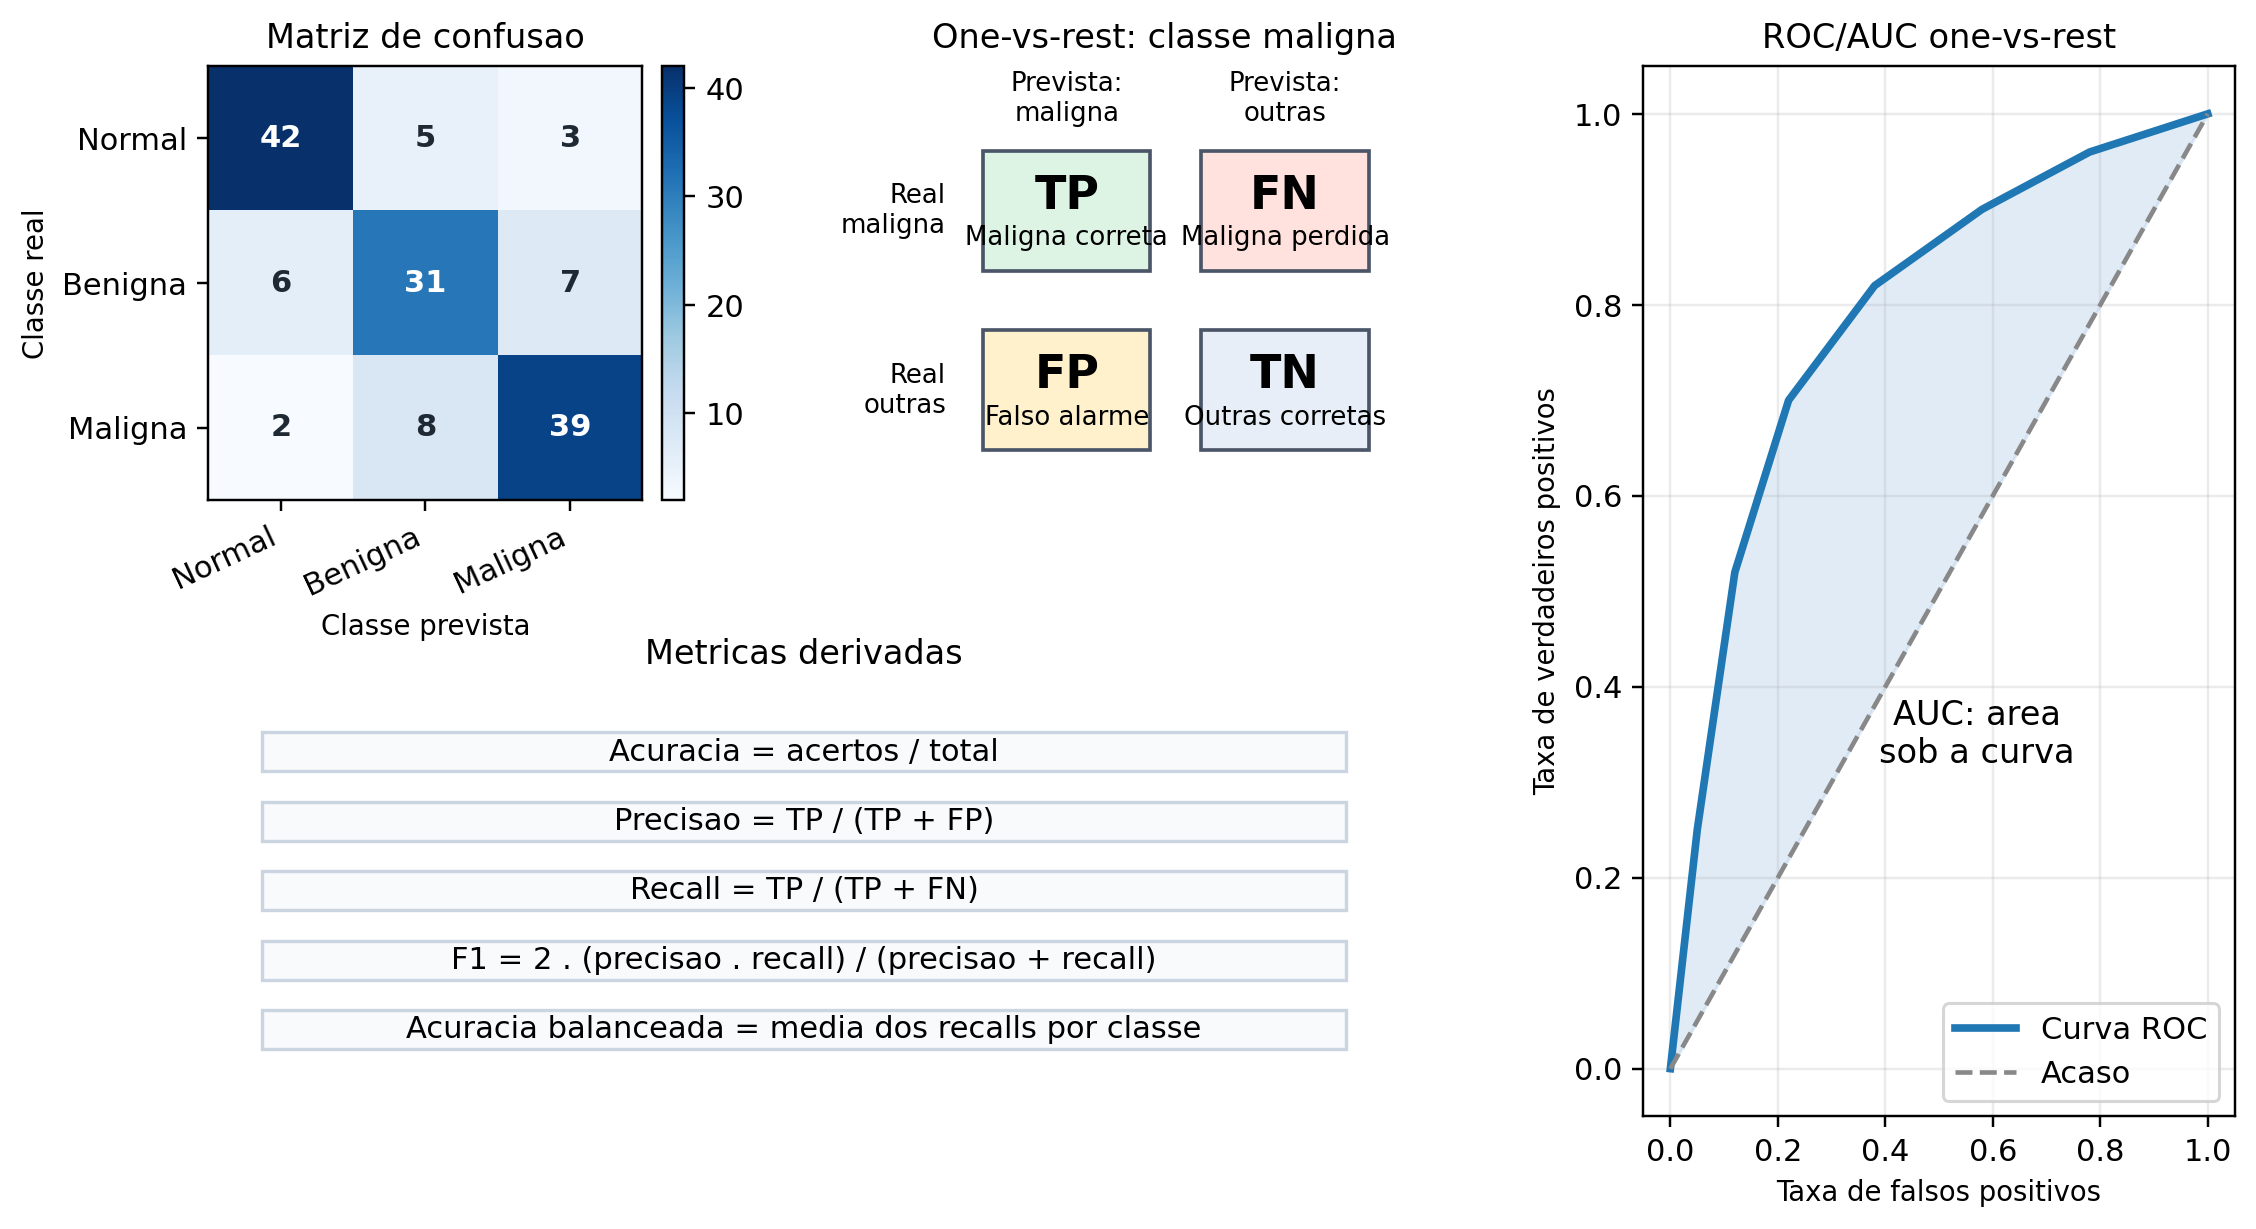
\includegraphics[width=\textwidth]{metricas_classificacao_exemplos.png}
    \legend{Fonte: Elaborado pelo autor (2026).}
\end{figure}

Portanto, a análise conjunta de acurácia, precisão, revocação, especificidade, Macro-F1, acurácia balanceada, AUC e matriz de confusão oferece uma caracterização rigorosa da capacidade de generalização dos modelos avaliados \cite{deisenroth2020mathematics}.

\subsection{Seleção de métricas em benchmarks multiclasse e desbalanceados}

A avaliação comparativa de modelos ao longo de múltiplos conjuntos de dados exige métricas que sejam simultaneamente sensíveis ao desempenho global e robustas a assimetrias na distribuição de classes. Embora a acurácia global indique a fração total de predições corretas, ela pode mascarar falhas severas em bases fortemente desbalanceadas, como GTSRB, FER2013 e SVHN, nas quais o acerto exclusivo nas classes majoritárias já produz valores elevados de acurácia.

Por esse motivo, este trabalho adota o Macro-F1 como métrica primária de comparação entre arquiteturas, funções de ativação e tamanhos de lote. Por calcular a média não ponderada dos F1-scores de todas as \(K\) classes, o Macro-F1 atribui peso idêntico a classes abundantes e raras, penalizando modelos que colapsam suas predições em poucas categorias. Complementarmente, a inspeção das matrizes de confusão e da variação de F1 por classe (\(\Delta\text{F1}\)) permite diagnosticar em quais categorias visuais específicas ocorrem ganhos ou perdas decorrentes da variação de hiperparâmetros ou da introdução de camadas quânticas.

\subsection{Métricas de custo computacional e estabilidade experimental}
\label{subsec:metricas_custo_estabilidade}

Além das métricas preditivas, a comparação entre uma CNN clássica de referência, uma CNN com gargalo clássico de controle e um modelo híbrido quântico-clássico exige o monitoramento sistemático do custo computacional e da estabilidade experimental. Para isso, o protocolo de telemetria registra o tempo médio por época, o tempo total acumulado de treinamento na campanha, a taxa de processamento de imagens por segundo (\textit{throughput}), a latência média de inferência por amostra ou lote, o consumo de memória, o número de parâmetros treináveis, o fator de aceleração (\textit{speedup}) entre sistemas operacionais e arquiteturas de hardware (Windows e macOS) e, no caso do modelo híbrido, o número de qubits, a profundidade do circuito parametrizado e o tempo despendido na simulação quântica.

A estabilidade experimental também deve ser avaliada porque redes neurais profundas e circuitos quânticos variacionais estão sujeitos à estocasticidade da inicialização de pesos, da amostragem de lotes (\textit{mini-batches}) e da otimização não convexa. Assim, os experimentos mantêm controle explícito de sementes pseudoaleatórias (\textit{seeds}), acompanhando a evolução época a época das curvas de perda e de Macro-F1 na validação para distinguir ganhos consistentes de flutuações pontuais.

\subsection{Comparação controlada entre modelos}
\label{subsec:comparacao_controlada_modelos}

Para que as conclusões científicas sejam válidas, a comparação entre diferentes configurações clássicas e híbridas deve ser conduzida sob o mesmo protocolo experimental. Isso significa utilizar exatamente as mesmas nove bases de dados, as mesmas definições de classes \(K\), as mesmas partições estratificadas de treino, validação e teste, o mesmo pré-processamento e os mesmos critérios de avaliação e seleção de \textit{checkpoints}. Dessa forma, as diferenças observadas em Macro-F1 ou em tempo de execução podem ser atribuídas diretamente ao fator investigado (arquitetura, função de ativação, tamanho de lote ou quantização), reduzindo variáveis de confusão externas.

Neste trabalho, a CNN clássica atua como linha de base (\textit{baseline}) principal; uma variante de CNN com gargalo clássico equivalente serve como controle metodológico para isolar o efeito da compressão dimensional; e a arquitetura híbrida quântico-clássica permite investigar se a substituição ou acoplamento desse gargalo a um circuito quântico variacional simulado altera a capacidade discriminativa, a dinâmica de convergência ou o custo operacional ao longo dos nove domínios visuais.

\section{Redes neurais e aprendizado profundo}

As redes neurais artificiais fazem parte do campo do aprendizado de máquina, no qual modelos computacionais são treinados para reconhecer padrões a partir de dados. Do ponto de vista matemático, um problema de aprendizado supervisionado pode ser representado por um conjunto de exemplos rotulados:

\[
\mathcal{D} = \{(x_1,y_1),(x_2,y_2),\ldots,(x_N,y_N)\},
\]

em que \(x_i\) representa uma entrada e \(y_i\) representa o rótulo associado a essa entrada. Em uma tarefa de classificação de imagens nos nove \textit{benchmarks} avaliados, \(x_i\) corresponde ao tensor numérico da imagem, enquanto \(y_i \in \{0, 1, \dots, K-1\}\) pertence ao conjunto das \(K\) classes definidas no domínio correspondente.

Segundo \citeonline{deisenroth2020mathematics}, a aprendizagem de máquina pode ser compreendida a partir de três componentes principais: dados, modelo e aprendizagem. Os dados precisam ser convertidos para uma representação numérica; o modelo descreve uma função parametrizada; e a aprendizagem corresponde ao ajuste desses parâmetros a partir dos dados disponíveis, com o objetivo de obter bom desempenho em exemplos ainda não vistos.

Assim, um modelo de aprendizado profundo pode ser descrito como uma função parametrizada:

\[
f_{\theta}: \mathbb{R}^{D} \rightarrow \mathbb{R}^{K},
\]

em que \(D\) representa a dimensão da entrada, \(K\) representa o número de classes (por exemplo, \(K=7\) no FER2013, \(K=10\) no MNIST, Fashion-MNIST, KMNIST, CIFAR-10 e SVHN, \(K=20\) no CIFAR-100 Coarse, \(K=43\) no GTSRB e \(K=47\) no EMNIST Balanced) e \(\theta\) representa o conjunto de parâmetros aprendidos pelo modelo.

O aprendizado profundo, ou \textit{deep learning}, diferencia-se de métodos tradicionais por utilizar múltiplas camadas de transformação não linear. Essas camadas permitem que o modelo aprenda representações hierárquicas dos dados. Em imagens, camadas iniciais tendem a capturar padrões simples, como bordas, contrastes e texturas locais, enquanto camadas mais profundas combinam essas informações em estruturas mais abstratas e semanticamente relevantes \cite{LeCun2015,goodfellow2016deep}.

Esse processo é essencial quando se avaliam múltiplos domínios visuais sob um mesmo protocolo experimental, pois permite que a mesma estrutura arquitetural adapte seus filtros internos desde contornos geométricos em caracteres manuscritos (\(28 \times 28 \times 1\)) até padrões cromáticos e texturais complexos em cenas urbanas, sinalização viária e objetos naturais (\(32 \times 32 \times 3\)).

\subsection{Redes neurais artificiais}

Uma rede neural artificial é composta por unidades matemáticas chamadas neurônios artificiais, organizadas em camadas. Cada neurônio recebe um conjunto de entradas, aplica uma combinação linear desses valores e, em seguida, utiliza uma função de ativação não linear. Considerando uma entrada \(x \in \mathbb{R}^{D}\), uma camada densa pode ser representada por:

\[
z = Wx + b,
\]

em que \(W \in \mathbb{R}^{M \times D}\) é a matriz de pesos, \(b \in \mathbb{R}^{M}\) é o vetor de vieses e \(z \in \mathbb{R}^{M}\) é o vetor de pré-ativações antes da aplicação da função não linear. Após a função de ativação \(\phi\), obtém-se:

\[
h = \phi(z) = \phi(Wx + b).
\]

A função de ativação é fundamental porque introduz não linearidade ao modelo. Sem ela, a composição de várias camadas lineares poderia ser reduzida a uma única transformação linear. Além da clássica função ReLU (\(\phi(z) = \max(0, z)\)), variações modernas como GELU (\textit{Gaussian Error Linear Unit}), SiLU/Swish (\(\phi(z) = z \cdot \sigma(z)\)), ELU (\textit{Exponential Linear Unit}) e LeakyReLU modificam a curvatura e o regime de propagação de gradientes para valores negativos de \(z\). A escolha comparativa entre essas funções de ativação desempenha papel central na campanha experimental deste trabalho, uma vez que impacta diretamente tanto a estabilidade de convergência e o Macro-F1 final quanto o custo aritmético de execução entre plataformas distintas (Windows e macOS).

Em uma rede com múltiplas camadas, a saída de uma camada é utilizada como entrada da camada seguinte. Assim, para uma camada \(l\), tem-se:

\[
h^{(l)} = \phi\left(W^{(l)}h^{(l-1)} + b^{(l)}\right),
\]

em que \(h^{(l-1)}\) representa a saída da camada anterior, \(W^{(l)}\) a matriz de pesos da camada atual e \(b^{(l)}\) o vetor de vieses. O conjunto de todos os pesos e vieses da rede compõe os parâmetros \(\theta\).

Em tarefas de classificação multiclasse, a última camada geralmente produz um vetor de escores \(s \in \mathbb{R}^{K}\), em que cada componente corresponde a uma classe. Para transformar esses escores em probabilidades, utiliza-se a função \textit{softmax}:

\[
p_k =
\frac{e^{s_k}}
{\sum_{j=0}^{K-1} e^{s_j}},
\]

em que \(p_k\) representa a probabilidade estimada para a classe \(k\). A classe prevista é dada por:

\[
\hat{y} = \arg\max_k p_k.
\]

O treinamento da rede consiste em ajustar os parâmetros \(\theta\) para reduzir a diferença entre a saída prevista e o rótulo verdadeiro. Para isso, define-se uma função de perda. Em problemas de classificação multiclasse, uma escolha comum é a entropia cruzada categórica:

\[
\mathcal{L}(y,\hat{p}) =
-\sum_{k=0}^{K-1} y_k \log(p_k),
\]

em que \(y_k\) representa o rótulo verdadeiro em codificação \textit{one-hot}. O objetivo do treinamento pode ser expresso como a minimização do risco empírico:

\[
R_{\text{emp}}(\theta) =
\frac{1}{N}
\sum_{i=1}^{N}
\mathcal{L}(y_i, f_{\theta}(x_i)).
\]

A atualização dos parâmetros é feita por métodos de otimização baseados em gradiente. De forma simplificada, uma etapa de gradiente descendente pode ser escrita como:

\[
\theta_{t+1}
=
\theta_t
-
\eta \nabla_{\theta}R_{\text{emp}}(\theta_t),
\]

em que \(\eta\) é a taxa de aprendizado e \(\nabla_{\theta}R_{\text{emp}}\) representa o gradiente da função de perda em relação aos parâmetros. Esse processo mostra que redes neurais dependem diretamente de fundamentos matemáticos como álgebra linear, cálculo vetorial, probabilidade e otimização \cite{deisenroth2020mathematics}.

O cálculo dos gradientes em redes profundas é realizado por meio da retropropagação do erro, ou \textit{backpropagation}. Esse algoritmo utiliza a regra da cadeia para calcular a contribuição de cada parâmetro para o erro final, permitindo que os pesos sejam atualizados progressivamente durante o treinamento. Assim, a rede aprende uma transformação capaz de mapear entradas numéricas para classes de saída.

\subsection{Redes neurais convolucionais}
\label{subsec:redes_neurais_convolucionais}

As redes neurais convolucionais, ou CNNs (\textit{Convolutional Neural Networks}), são arquiteturas especializadas no processamento de dados com estrutura espacial, como imagens. Diferentemente das redes densas, nas quais todos os neurônios de uma camada se conectam a todos os neurônios da camada seguinte, as CNNs exploram a organização local dos pixels por meio de filtros convolucionais. Essa característica reduz o número de parâmetros, preserva relações espaciais e permite que a rede aprenda padrões visuais relevantes diretamente a partir dos dados.

Em uma imagem digital, pixels vizinhos geralmente possuem relações importantes entre si. Bordas, texturas, contrastes, contornos geométricos e estruturas locais não aparecem como valores isolados, mas como padrões distribuídos em regiões vizinhas da imagem. Por esse motivo, as CNNs são especialmente adequadas para tarefas de visão computacional, pois aplicam filtros sobre pequenas janelas da imagem, extraindo informações locais que são combinadas progressivamente ao longo das camadas.

Matematicamente, uma convolução discreta pode ser entendida como a aplicação de um filtro, ou \textit{kernel}, sobre uma imagem. Considerando uma imagem bidimensional \(I\) e um filtro \(K\) de tamanho \((2a+1) \times (2b+1)\), a saída da convolução em uma posição \((i,j)\) pode ser representada por:

\[
S(i,j) =
\sum_{m=-a}^{a}
\sum_{n=-b}^{b}
K(m,n)\cdot I(i+m,j+n).
\]

Nessa expressão, \(I(i+m,j+n)\) representa os pixels vizinhos à posição analisada, enquanto \(K(m,n)\) representa os pesos do filtro. O resultado \(S(i,j)\) corresponde à resposta do filtro naquela região da imagem. Assim, cada posição do mapa de saída resume uma combinação ponderada de uma vizinhança local da imagem original.

A Figura~\ref{fig:convolucao_pooling} apresenta uma representação esquemática da aplicação de um filtro convolucional sobre uma imagem e da etapa posterior de \textit{pooling}. A convolução percorre a imagem por regiões locais e produz um mapa de características; em seguida, o \textit{pooling} reduz a dimensão espacial desse mapa, preservando informações consideradas mais relevantes.

\begin{figure}[H]
    \centering
    \caption{Representação esquemática das operações de convolução e \textit{pooling} em uma rede neural convolucional.}
    \label{fig:convolucao_pooling}
    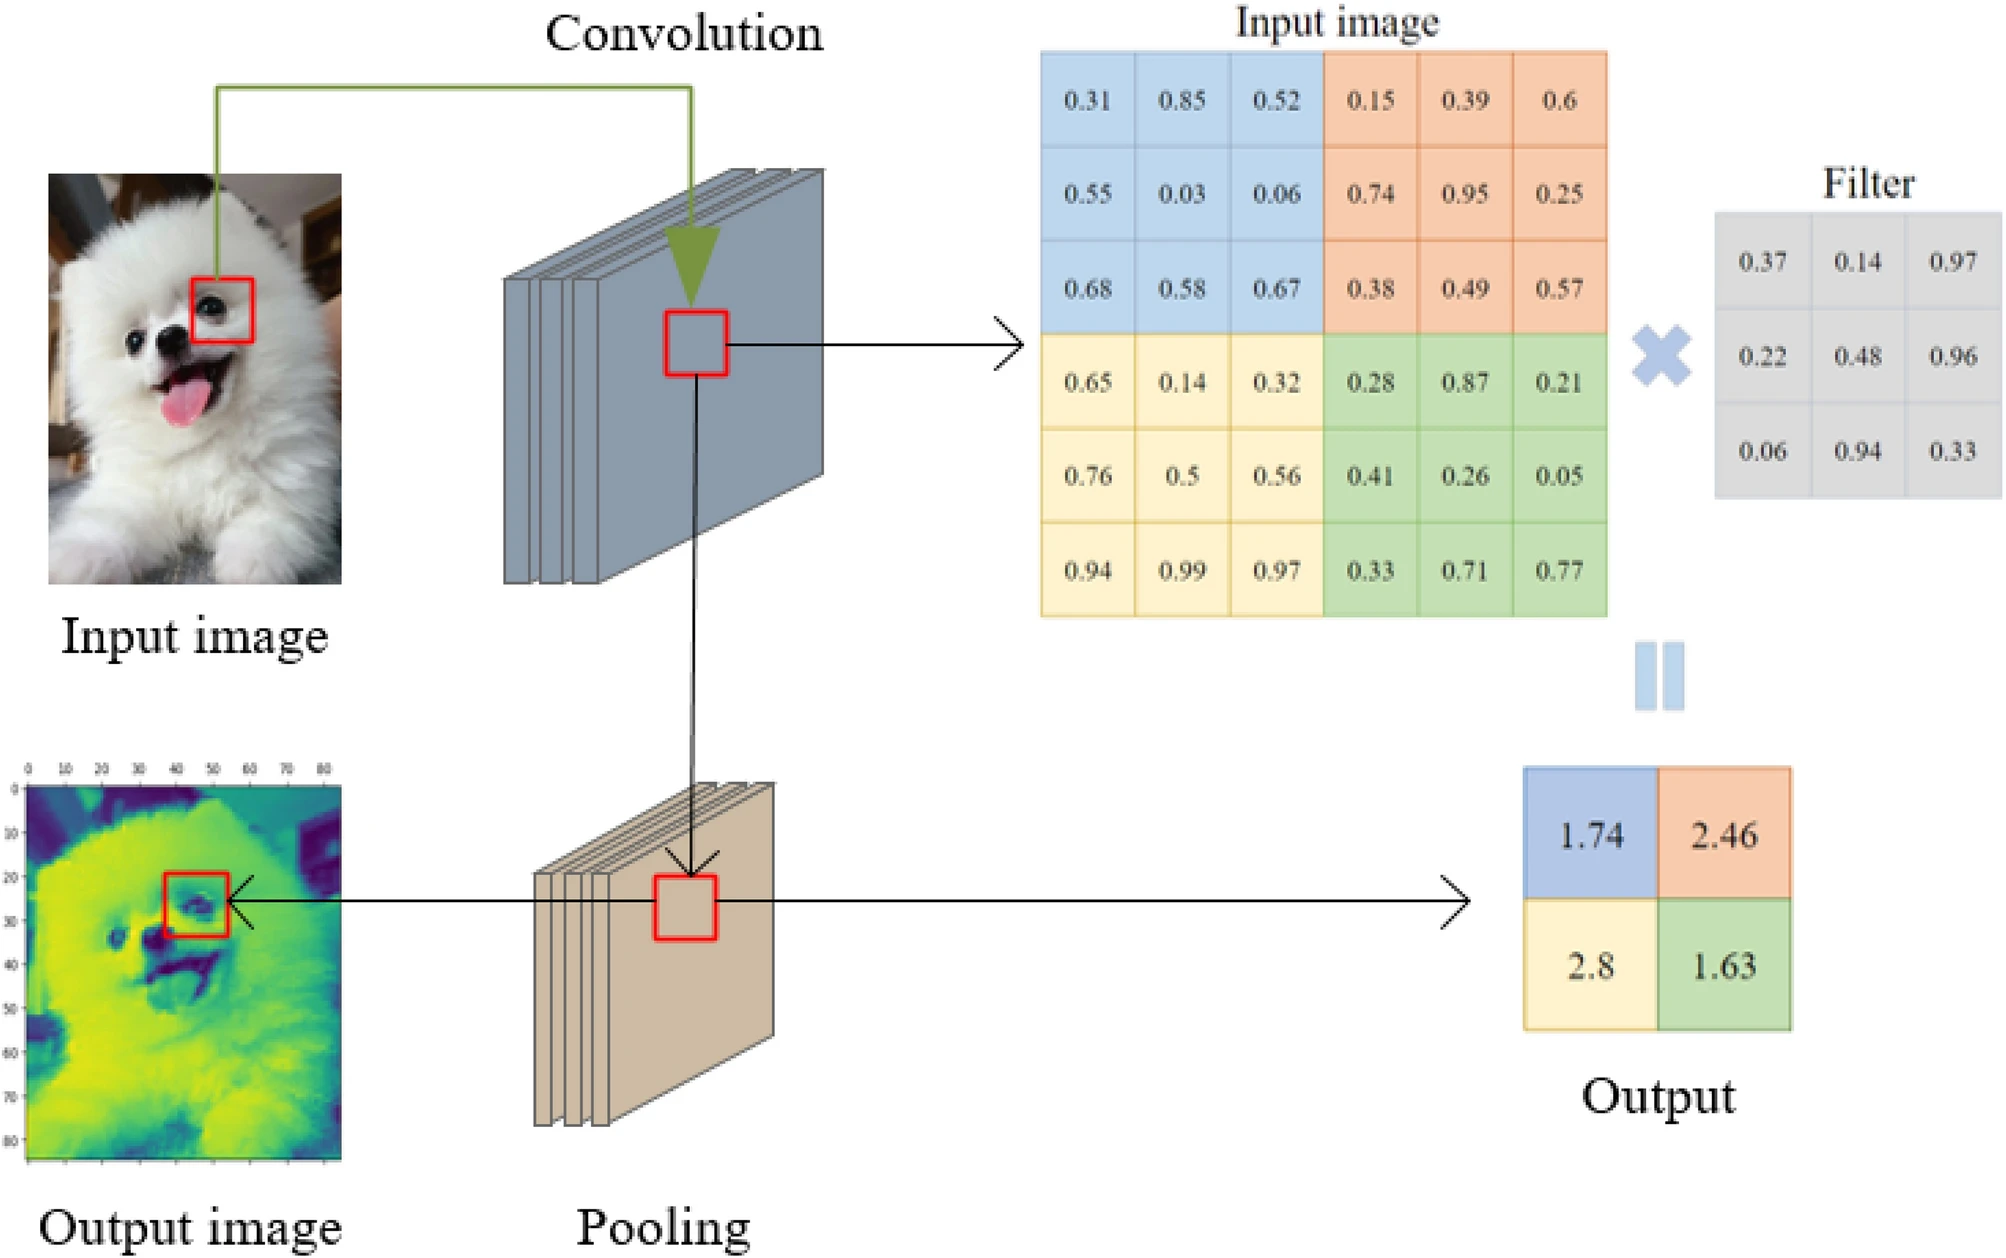
\includegraphics[width=0.85\textwidth]{convolutional-pooling.png}
    \legend{Fonte: adaptado de Zhao e Zhang \cite{zhao2024improvedpooling}.}
\end{figure}

Em uma CNN, os valores dos filtros não são definidos manualmente. Eles são aprendidos durante o treinamento, de acordo com a função de perda e com os dados apresentados à rede. Nas primeiras camadas, os filtros tendem a capturar padrões simples, como bordas, contornos, regiões de contraste e texturas. Nas camadas intermediárias e profundas, esses padrões são combinados em representações mais complexas, capazes de descrever estruturas maiores e mais abstratas.

Em uma camada convolucional, vários filtros são aplicados sobre a imagem ou sobre os mapas de características produzidos pela camada anterior. Cada filtro gera um mapa de características diferente, destacando um tipo de padrão visual. Para uma entrada com múltiplos canais, a saída de um filtro \(r\) pode ser escrita como:

\[
S_r(i,j) =
\sum_{c=1}^{C}
\sum_{m=-a}^{a}
\sum_{n=-b}^{b}
K_{r,c}(m,n)\cdot I_c(i+m,j+n) + b_r,
\]

em que \(C\) é o número de canais de entrada, \(r\) identifica o filtro utilizado, \(K_{r,c}\) representa os pesos do filtro \(r\) aplicados ao canal \(c\), e \(b_r\) é o viés associado ao filtro. Em bases coloridas no formato RGB (como CIFAR-10, CIFAR-100, SVHN e GTSRB), tem-se \(C=3\). Já em bases monocromáticas em escala de cinza (como MNIST, Fashion-MNIST, KMNIST, EMNIST e FER2013), tem-se \(C=1\), pois há apenas um canal de intensidade.

Após a convolução, aplica-se normalmente uma função de ativação não linear, como a ReLU (\textit{Rectified Linear Unit}):

\[
ReLU(x) = \max(0,x).
\]

Essa função mantém valores positivos e zera valores negativos, introduzindo não linearidade ao modelo. Sem funções de ativação, a composição de várias camadas convolucionais e densas poderia ser reduzida a uma transformação linear, limitando a capacidade da rede de representar padrões complexos.

Depois da ativação, é comum utilizar uma camada de \textit{pooling}. O \textit{pooling} reduz a dimensão espacial dos mapas de características, diminuindo o custo computacional e tornando a representação mais compacta. Uma operação comum é o \textit{max pooling}, definida por:

\[
P(i,j) =
\max_{(m,n)\in R_{ij}}
S(m,n),
\]

em que \(R_{ij}\) representa uma região local do mapa de características. Nesse caso, a saída corresponde ao maior valor dentro da janela analisada. Também existe o \textit{average pooling}, que calcula a média dos valores da região. \citeonline{zhao2024improvedpooling} destacam que o \textit{pooling} é importante para reduzir as dimensões espaciais e o volume de dados, mas também pode causar perda de informações, especialmente quando detalhes finos são relevantes.

Esse ponto é particularmente importante em \textit{benchmarks} de baixa resolução espacial (\(28 \times 28\) ou \(32 \times 32\) pixels). Reduções espaciais excessivas podem suprimir traços caligráficos sutis no KMNIST e EMNIST, pequenos elementos de sinalização no GTSRB ou microexpressões faciais no FER2013. Portanto, a profundidade e o escalonamento espacial dos blocos convolucionais devem equilibrar compressão e preservação de detalhes discriminativos.

A Figura~\ref{fig:feature_maps} mostra uma visualização de mapas de características produzidos em diferentes blocos convolucionais. Observa-se que as primeiras camadas ainda preservam boa parte da estrutura visual da imagem original, enquanto camadas mais profundas produzem ativações mais abstratas e espacialmente reduzidas. Esse comportamento ilustra a ideia de aprendizado hierárquico em CNNs: padrões simples são aprendidos nas camadas iniciais e combinados em representações mais complexas nas camadas posteriores.

\begin{figure}[H]
    \centering
    \caption{Exemplo de visualização de mapas de características em diferentes blocos convolucionais. As camadas iniciais tendem a preservar bordas, texturas e contornos, enquanto camadas mais profundas representam padrões mais abstratos.}
    \label{fig:feature_maps}
    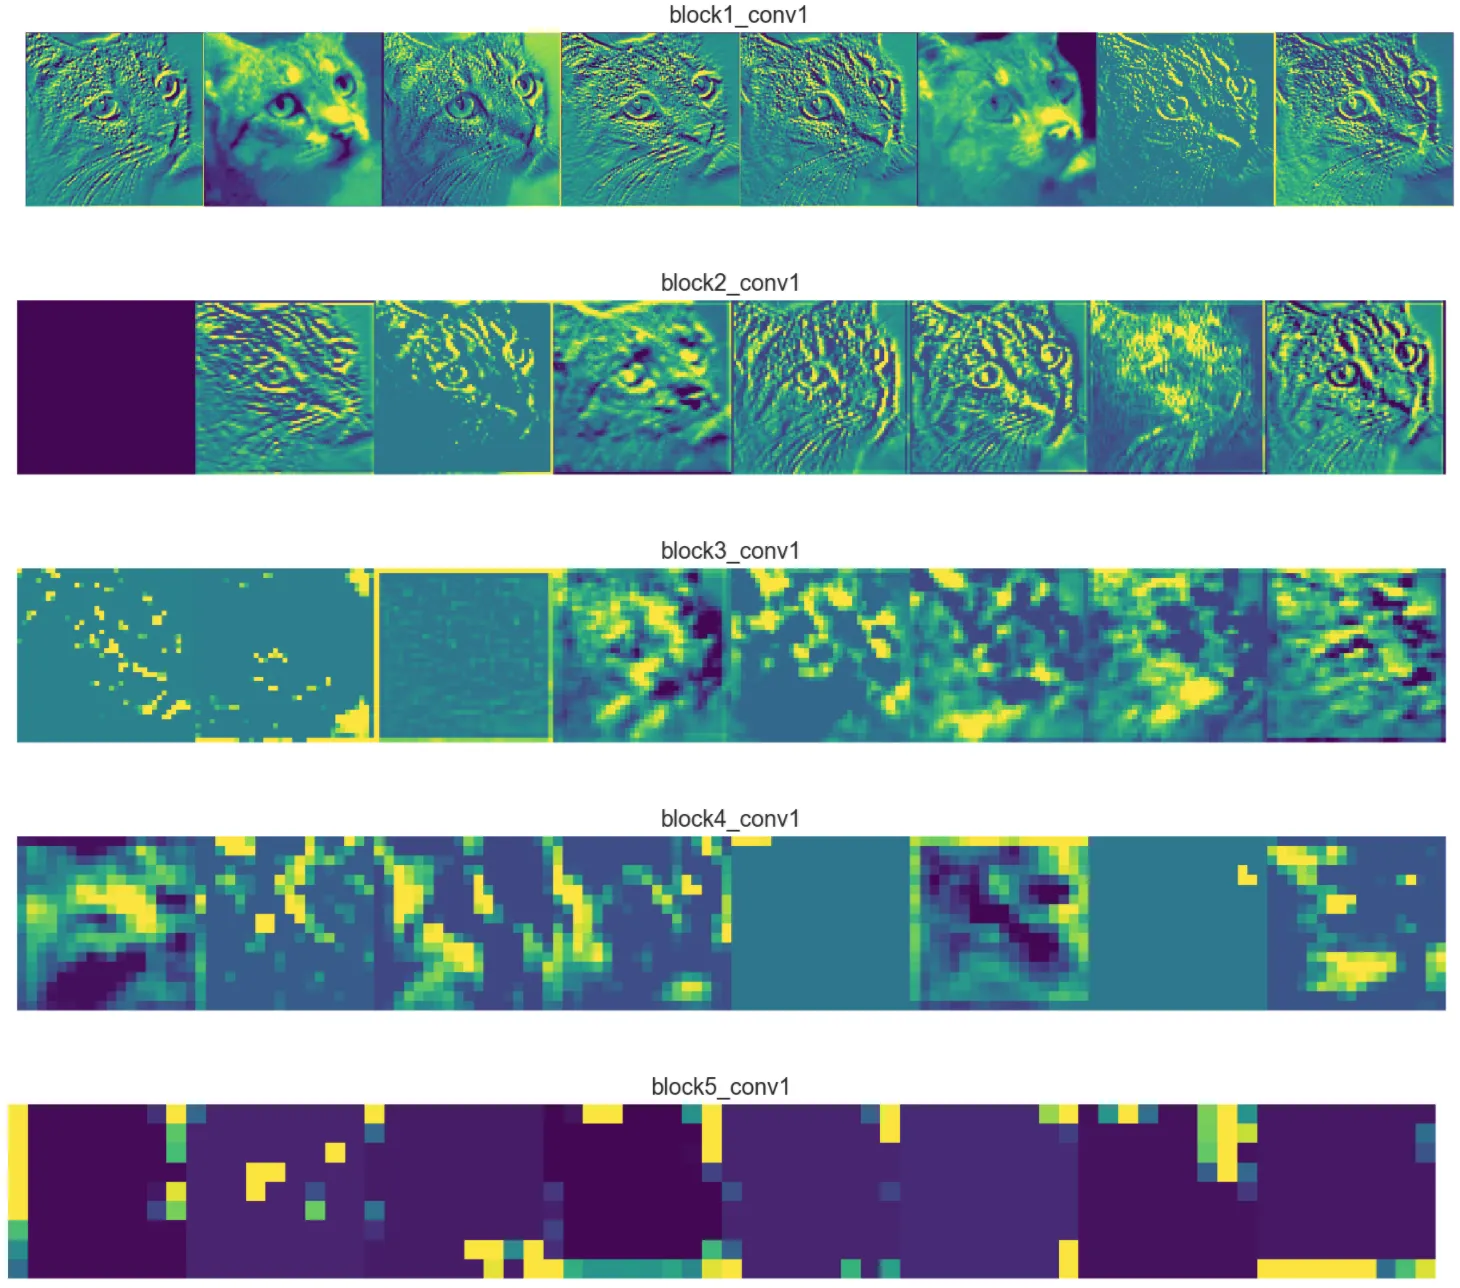
\includegraphics[width=\textwidth]{feature-map-converted.png}
    \legend{Fonte: adaptado de Hesaraki \cite{hesaraki2023featuremap}.}
\end{figure}

O desenvolvimento das CNNs profundas foi fundamental para o avanço da visão computacional. Arquiteturas como AlexNet, VGG, GoogLeNet/Inception e ResNet demonstraram que redes convolucionais profundas podem aprender representações hierárquicas altamente eficazes para classificação de imagens \cite{szegedy2014going,he2016resnet}. \citeonline{szegedy2014going} mostraram que é possível aumentar profundidade e largura da rede mantendo preocupação com eficiência computacional, princípio essencial em campanhas experimentais extensas envolvendo múltiplos conjuntos de dados.

A Figura~\ref{fig:convolucao_2mais1d} apresenta uma decomposição de convolução espaço-temporal em uma convolução espacial e uma convolução temporal. Embora este trabalho utilize imagens estáticas bidimensionais nos nove conjuntos de dados avaliados, e não sequências temporais, a figura ilustra como diferentes operadores convolucionais podem ser estruturados de acordo com a dimensionalidade do sinal. Em imagens 2D, o filtro percorre altura e largura; em dados volumétricos ou sequenciais, a convolução incorpora também profundidade ou tempo.

\begin{figure}[H]
    \centering
    \caption{Exemplo de decomposição de uma convolução espaço-temporal em convolução espacial e temporal. No contexto deste trabalho, a figura ilustra a generalidade do operador convolucional, sendo os nove \textit{benchmarks} avaliados compostos por imagens estáticas bidimensionais.}
    \label{fig:convolucao_2mais1d}
    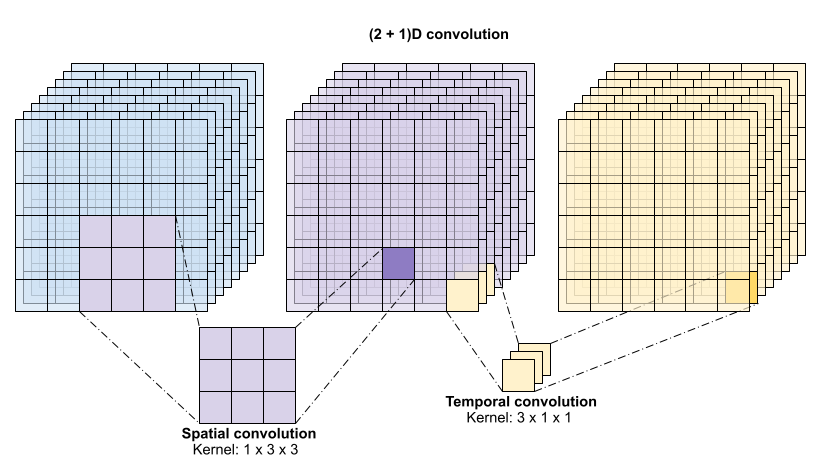
\includegraphics[width=0.70\textwidth]{2plus1CNN-converted.png}
    \legend{Fonte: Elaborado pelo autor (2026).}
\end{figure}

Dessa forma, a estrutura canônica de uma CNN combina camadas convolucionais, normalização em lote (\textit{batch normalization}), funções de ativação não lineares, camadas de \textit{pooling}, regularização por \textit{dropout} e uma cabeça de classificação que mapeia as características extraídas para a distribuição de probabilidades entre as \(K\) classes do problema.

\subsection{CNNs aplicadas a múltiplos domínios de visão computacional e eficiência de execução}

As redes neurais convolucionais consolidaram-se como a arquitetura de referência para classificação de imagens em múltiplos domínios devido ao compartilhamento de pesos e à invariância local a translações. Ao aplicar filtros convolucionais sucessivos seguidos de funções de ativação não lineares e operações de redução espacial (\textit{pooling}), a rede adapta seus mapas de características tanto a traços morfológicos simples em imagens monocromáticas (\(28 \times 28 \times 1\)) quanto a texturas cromáticas complexas em imagens naturais (\(32 \times 32 \times 3\)).

Além da topologia das camadas, o comportamento prático de uma CNN em campanhas extensas de treinamento é fortemente influenciado pelo dimensionamento do lote (\textit{batch size}) e pela precisão numérica dos parâmetros. Lotes menores (como 32 ou 64) introduzem maior variância estocástica na estimativa do gradiente, o que pode atuar como regularizador implícito e favorecer a generalização em determinadas bases, porém reduz o paralelismo de hardware e eleva o tempo por época. Em contrapartida, lotes maiores (como 128 ou 256) maximizam a taxa de processamento (\textit{throughput}) em GPUs, mas podem convergir para mínimos mais agudos caso a taxa de aprendizado não seja devidamente ajustada. De modo complementar, técnicas de quantização de modelos permitem comprimir a representação numérica dos pesos e ativações (por exemplo, de ponto flutuante de 32 bits para inteiros de 8 bits ou ponto flutuante de 16 bits), buscando reduzir a latência de inferência e o uso de memória sem degradação significativa no Macro-F1 \cite{goodfellow2016deep,zandieh2025turboquant}.

\subsection{Aumento de dados, regularização e overfitting}
\label{subsec:aumento_regularizacao_overfitting}

O treinamento de redes neurais profundas exige cuidado com a capacidade de generalização do modelo. Em aprendizado supervisionado, o objetivo não é apenas reduzir o erro sobre os dados de treinamento, mas obter bom desempenho em exemplos ainda não vistos. Esse princípio é especialmente relevante quando se avaliam bases com alto número de classes ou forte desbalanceamento, pois modelos de alta capacidade podem memorizar padrões de fundo, artefatos de iluminação ou peculiaridades amostrais do conjunto de treino.

Em termos matemáticos, considera-se um conjunto de treinamento:

\[
\mathcal{D}_{train} = \{(x_1,y_1),(x_2,y_2),\ldots,(x_N,y_N)\},
\]

em que \(x_i\) representa uma imagem e \(y_i\) seu respectivo rótulo. O treinamento busca ajustar os parâmetros \(\theta\) de um modelo \(f_{\theta}\) minimizando uma função de perda média, também chamada de risco empírico:

\[
R_{\text{emp}}(\theta) =
\frac{1}{N}
\sum_{i=1}^{N}
\mathcal{L}(y_i, f_{\theta}(x_i)).
\]

Entretanto, minimizar excessivamente essa perda no conjunto de treino não garante bom desempenho em dados novos. Quando o modelo apresenta baixo erro no treino, mas erro elevado na validação ou no teste, ocorre o fenômeno conhecido como \textit{overfitting}, ou sobreajuste. Nesse caso, a rede aprende detalhes específicos dos exemplos de treinamento, reduzindo sua capacidade de generalização. Por outro lado, quando o modelo é simples demais ou treinado de forma insuficiente, pode ocorrer \textit{underfitting}, situação em que o desempenho é baixo tanto no treino quanto na validação.

Uma forma de reduzir o sobreajuste é aplicar regularização. A regularização introduz restrições ou penalizações ao processo de aprendizagem, buscando impedir que o modelo se ajuste de forma excessiva aos dados de treino. Uma formulação comum consiste em adicionar um termo de penalização à função objetivo:

\[
J(\theta) =
\frac{1}{N}
\sum_{i=1}^{N}
\mathcal{L}(y_i, f_{\theta}(x_i))
+
\lambda \Omega(\theta),
\]

em que \(\Omega(\theta)\) é o termo de regularização e \(\lambda\) controla a intensidade da penalização. Quando se utiliza regularização \(L_2\) (\textit{weight decay}), por exemplo, a penalização é definida como:

\[
\Omega(\theta) = \|\theta\|_2^2.
\]

Nesse caso, pesos muito altos são penalizados, incentivando o modelo a encontrar soluções mais suaves e menos dependentes de parâmetros extremos. Essa estratégia pode melhorar a generalização, pois reduz a tendência da rede de memorizar detalhes específicos dos dados de treino \cite{goodfellow2016deep}.

Outra técnica amplamente utilizada é o \textit{dropout}. Durante o treinamento, o \textit{dropout} desativa aleatoriamente uma proporção dos neurônios de uma camada, forçando a rede a distribuir melhor a informação entre diferentes unidades. Se \(h\) representa o vetor de ativações de uma camada, o \textit{dropout} pode ser representado de forma simplificada como:

\[
\tilde{h} = m \odot h,
\]

em que \(m\) é uma máscara binária aleatória, \(\odot\) representa o produto elemento a elemento e \(\tilde{h}\) corresponde às ativações após a aplicação da máscara. Essa técnica reduz a dependência excessiva de neurônios específicos e contribui para tornar o modelo mais robusto.

Além da regularização dos parâmetros, outra estratégia essencial é o aumento de dados, ou \textit{data augmentation}. Essa técnica consiste em gerar variações artificiais das imagens de treinamento por meio de transformações que preservam o rótulo da amostra. Matematicamente, uma imagem \(x_i\) pode ser transformada por uma função \(T\), produzindo uma nova amostra:

\[
x_i' = T(x_i),
\]

em que \(x_i'\) mantém o mesmo rótulo \(y_i\), desde que a transformação respeite a semântica da classe.

No contexto de \textit{benchmarks} heterogêneos de visão computacional, a estratégia de aumento de dados (\textit{data augmentation}) deve respeitar as invariâncias semânticas de cada domínio. Enquanto pequenos deslocamentos horizontais/verticais, recortes aleatórios (\textit{random crops}), ajustes leves de brilho e contraste e rotações sutis preservam o rótulo na maioria das bases, espelhamentos horizontais (\textit{horizontal flips}) são válidos para objetos naturais (CIFAR-10/100), artigos de vestuário simétricos (Fashion-MNIST) e faces (FER2013), mas inválidos para dígitos, caracteres e determinadas placas de trânsito (MNIST, KMNIST, EMNIST, SVHN e GTSRB), pois inverteriam a orientação canônica do símbolo. A Figura~\ref{fig:aumento_dados_exemplos} ilustra exemplos de transformações controladas aplicadas a uma imagem em escala de cinza para ampliar a diversidade do conjunto de treinamento sem descaracterizar o padrão visual. Assim, o controle experimental entre regimes sem aumento de dados e com aumento controlado é fundamental para isolar o ganho real de regularização em cada arquitetura.

\begin{figure}[H]
    \centering
    \caption{Exemplos de aumento de dados por transformações leves aplicadas a uma imagem sintética em escala de cinza, ilustrando variações controladas que ampliam a diversidade do conjunto de treinamento preservando o rótulo da amostra.}
    \label{fig:aumento_dados_exemplos}
    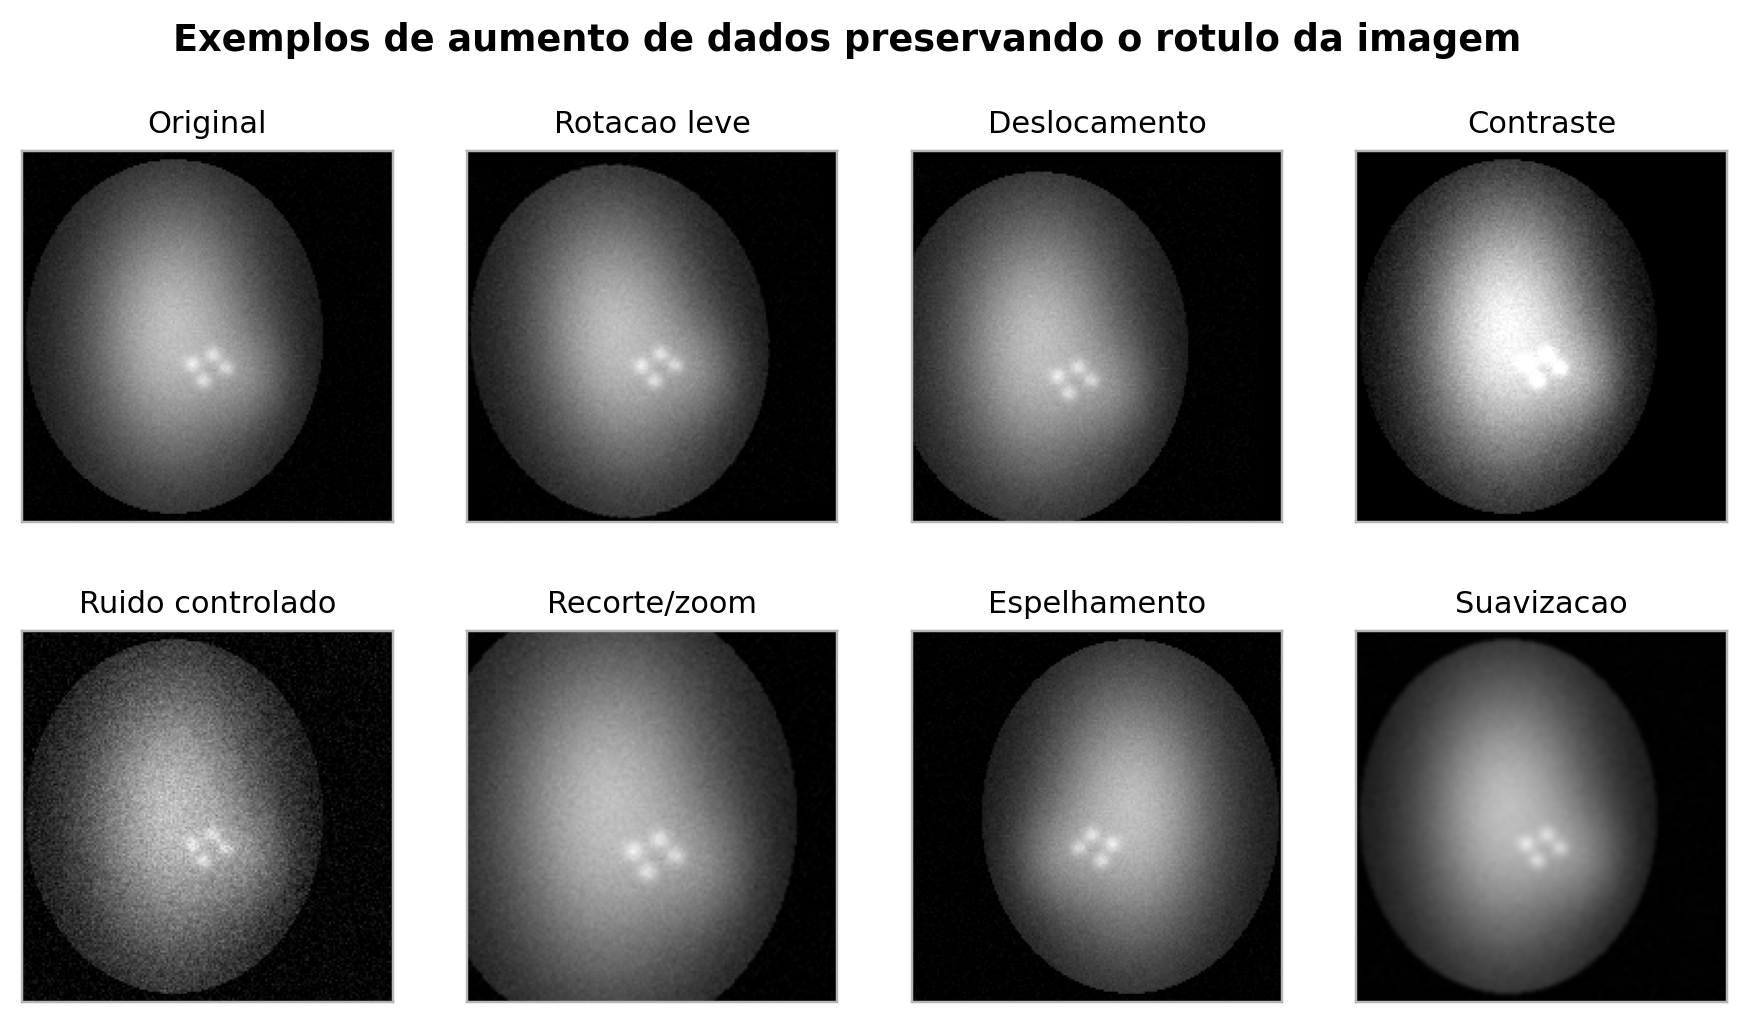
\includegraphics[width=\textwidth]{aumento_dados_exemplos.png}
    \legend{Fonte: Elaborado pelo autor (2026).}
\end{figure}

Outra técnica relacionada à regularização é o \textit{early stopping}. Nesse procedimento, o desempenho do modelo é monitorado no conjunto de validação durante o treinamento. Quando a perda de validação (ou o Macro-F1 de validação) deixa de melhorar por um número definido de épocas, o treinamento é interrompido ou o melhor \textit{checkpoint} é restaurado. Essa estratégia evita que o modelo continue reduzindo a perda de treino enquanto degrada sua capacidade de generalização:

\[
\mathcal{L}_{train} \downarrow
\quad \text{e} \quad
\mathcal{L}_{val} \uparrow.
\]

Portanto, aumento de dados controlado por domínio, regularização \(L_2\), \textit{dropout}, normalização em lote e seleção pelo melhor estado de validação constituem estratégias complementares indispensáveis para garantir estabilidade e reprodutibilidade ao comparar modelos clássicos e híbridos nos nove conjuntos de dados.

\subsection{Explicabilidade e interpretação de representações em CNNs}

A interpretabilidade das representações internas aprendidas por redes neurais profundas é um aspecto relevante em visão computacional, uma vez que permite auditar se as decisões de um classificador baseiam-se em atributos morfológicos legítimos do objeto ou em correlações espúrias do fundo da imagem. Embora CNNs alcancem elevado desempenho preditivo, suas decisões resultam da composição de múltiplas camadas de transformação não linear.

Uma das técnicas utilizadas para auxiliar a inspeção espacial de CNNs é o Grad-CAM (\textit{Gradient-weighted Class Activation Mapping}) \cite{selvaraju2020gradcam}. Essa abordagem gera mapas de ativação ponderados por gradientes que destacam quais regiões espaciais da imagem exerceram maior influência na predição de determinada classe \(k\). Em \textit{benchmarks} de visão computacional, análises de mapas de características e de atenção espacial complementam a inspeção de matrizes de confusão e de resíduos por classe (\(\Delta\text{F1}\)), auxiliando a compreender como diferentes escolhas arquiteturais e de hiperparâmetros afetam a extração de padrões visuais.

\section{Computação quântica e aprendizado de máquina quântico}

A computação quântica é um paradigma computacional baseado em princípios da mecânica quântica, como superposição, emaranhamento, interferência e medição probabilística \cite{nielsen2010quantum}. Diferentemente da computação clássica, que utiliza bits para representar informações nos estados 0 ou 1, a computação quântica utiliza qubits, que podem assumir combinações lineares desses estados. Essa diferença permite representar e manipular informações em espaços vetoriais complexos de alta dimensão, chamados espaços de Hilbert.

O aprendizado de máquina quântico, ou \textit{Quantum Machine Learning} (QML), investiga como recursos da computação quântica podem ser utilizados em tarefas de aprendizado de máquina, como classificação, regressão, agrupamento e redução de dimensionalidade. Em dispositivos quânticos atuais, caracterizados por número limitado de qubits, ruído e restrições de profundidade dos circuitos, uma das abordagens mais estudadas é a construção de modelos híbridos quântico-clássicos. Nesses modelos, parte do processamento é realizada por componentes clássicos e parte por circuitos quânticos parametrizados \cite{biamonte2017qml,preskill2018nisq,cerezo2021variational}.

No contexto deste trabalho, o interesse principal está na aplicação de modelos híbridos à classificação supervisionada de imagens ao longo de múltiplos \textit{benchmarks} de visão computacional. Como mesmo imagens compactas possuem centenas ou milhares de valores de intensidade, a aplicação direta de circuitos quânticos a todos os pixels ainda é limitada. Por isso, arquiteturas híbridas utilizam camadas convolucionais clássicas para extrair e comprimir características espaciais e, posteriormente, inserem um bloco quântico variacional responsável por processar esse vetor latente antes da camada final de decisão.

\subsection{Qubits, superposição, emaranhamento e medição}

O qubit é a unidade básica de informação quântica. Enquanto um bit clássico pode assumir apenas um dos valores 0 ou 1, um qubit pode ser representado como uma combinação linear dos estados base \(\ket{0}\) e \(\ket{1}\):

\[
\ket{\psi} = \alpha\ket{0} + \beta\ket{1},
\]

em que \(\alpha\) e \(\beta\) são amplitudes complexas que satisfazem a condição de normalização:

\[
|\alpha|^2 + |\beta|^2 = 1.
\]

Os valores \(|\alpha|^2\) e \(|\beta|^2\) representam as probabilidades de observar, após a medição, os estados \(\ket{0}\) e \(\ket{1}\), respectivamente. Assim, antes da medição, o qubit pode estar em superposição; após a medição, o resultado observado será clássico, assumindo um dos estados possíveis.

Na prática, circuitos quânticos são descritos por sequências de portas aplicadas a qubits e, ao final, por operações de medição que produzem bits clássicos ou valores esperados. A documentação da IBM Quantum para o Qiskit apresenta diferentes formas de visualização desses circuitos, incluindo representações geradas por Matplotlib e por \LaTeX, como ilustrado na Figura~\ref{fig:ibm_visualizacao_circuito}.

\begin{figure}[H]
    \centering
    \caption{Exemplo de circuito quântico com portas \(H\), \(X\), CNOT e operações de medição, apresentado na documentação da IBM Quantum sobre visualização de circuitos no Qiskit.}
    \label{fig:ibm_visualizacao_circuito}
    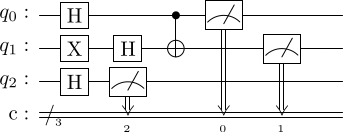
\includegraphics[width=0.72\textwidth]{ibm_visualize_circuits_latex.png}
    \legend{Fonte: IBM Quantum \cite{ibmQuantumVisualizeCircuits2026}.}
\end{figure}

Para um sistema com \(n\) qubits, o estado quântico pertence a um espaço de dimensão \(2^n\). Por exemplo, dois qubits possuem quatro estados base:

\[
\ket{00}, \ket{01}, \ket{10}, \ket{11}.
\]

De forma geral, um estado de dois qubits pode ser representado por:

\[
\ket{\psi} =
\alpha_{00}\ket{00}
+
\alpha_{01}\ket{01}
+
\alpha_{10}\ket{10}
+
\alpha_{11}\ket{11},
\]

com a condição:

\[
|\alpha_{00}|^2 +
|\alpha_{01}|^2 +
|\alpha_{10}|^2 +
|\alpha_{11}|^2 = 1.
\]

Esse crescimento exponencial do espaço de estados é uma das razões pelas quais a computação quântica desperta interesse em problemas de alta complexidade. Entretanto, esse mesmo crescimento também torna a simulação clássica de circuitos quânticos rapidamente custosa.

Outro fenômeno importante é o emaranhamento. Um estado é dito emaranhado quando não pode ser decomposto como produto tensorial de estados individuais dos qubits. Um exemplo clássico é o estado de Bell:

\[
\ket{\Phi^+} =
\frac{1}{\sqrt{2}}
(\ket{00} + \ket{11}).
\]

Nesse caso, os qubits apresentam correlações que não podem ser descritas apenas como estados independentes. A medição de um qubit afeta a descrição do estado global do sistema, produzindo correlações probabilísticas fortes entre os resultados.

A medição é o processo que transforma informação quântica em informação clássica. Em modelos de aprendizado de máquina quântico, as medições são fundamentais, pois as saídas do circuito geralmente são obtidas por probabilidades de medição ou por valores esperados de observáveis. Por exemplo, pode-se medir o valor esperado do operador de Pauli-Z em um qubit:

\[
\langle Z \rangle =
\bra{\psi} Z \ket{\psi}.
\]

Esse valor esperado pode ser utilizado como uma característica numérica de saída do circuito quântico e, posteriormente, alimentar uma camada clássica de classificação.

\subsection{Portas e circuitos quânticos parametrizados}

As portas quânticas são operações matemáticas aplicadas sobre qubits. Diferentemente de muitas operações clássicas, as portas quânticas são representadas por matrizes unitárias, isto é, matrizes \(U\) que satisfazem:

\[
U^\dagger U = I,
\]

em que \(U^\dagger\) representa a conjugada transposta de \(U\) e \(I\) é a matriz identidade. Essa propriedade garante que a norma do estado quântico seja preservada durante a evolução do circuito.

Entre as portas quânticas mais comuns estão as portas de Pauli \(X\), \(Y\) e \(Z\), a porta Hadamard \(H\), portas de rotação e portas controladas, como CNOT e CZ. A porta Hadamard, por exemplo, é frequentemente utilizada para criar superposição:

\[
H\ket{0} =
\frac{1}{\sqrt{2}}
(\ket{0} + \ket{1}).
\]

Portas de rotação são especialmente importantes em modelos variacionais, pois dependem de parâmetros ajustáveis. Uma rotação em torno do eixo \(Y\), por exemplo, pode ser representada por:

\[
R_Y(\theta) =
e^{-i\frac{\theta}{2}Y}.
\]

De modo geral, um circuito quântico parametrizado pode ser representado por uma operação unitária \(U(\theta)\), em que \(\theta\) representa um conjunto de parâmetros treináveis. Um circuito formado por várias camadas pode ser escrito como:

\[
U(\theta) =
U_L(\theta_L)
U_{L-1}(\theta_{L-1})
\cdots
U_1(\theta_1).
\]

Essa estrutura é análoga, em certo sentido, às redes neurais clássicas, nas quais diferentes camadas aplicam transformações sucessivas aos dados. No caso quântico, as transformações são operações unitárias aplicadas sobre estados quânticos.

Em modelos híbridos, os parâmetros do circuito são ajustados por um otimizador clássico. O circuito quântico calcula uma saída, normalmente associada a valores esperados de observáveis, e essa saída é usada para computar uma função de custo. Em seguida, um algoritmo clássico atualiza os parâmetros do circuito. Esse ciclo forma a base dos algoritmos variacionais quânticos \cite{cerezo2021variational}.

\subsection{Codificação de dados clássicos em estados quânticos}

Para que dados clássicos sejam processados por um circuito quântico, é necessário convertê-los em estados quânticos ou em parâmetros de portas quânticas. Esse processo é chamado de codificação, incorporação ou \textit{embedding} dos dados \cite{schuld2021effect}. A escolha da codificação é uma etapa central em QML, pois determina como a informação clássica será representada no espaço quântico.

Uma forma simples de codificação é a codificação por ângulo (\textit{angle embedding}). Nesse caso, os atributos clássicos de uma entrada \(x = [x_1, x_2, \ldots, x_d]\) são usados como ângulos de rotação em portas quânticas. Por exemplo, pode-se aplicar uma rotação em cada qubit:

\[
\ket{\psi(x)}
=
\prod_{j=1}^{d}
R_Y(x_j)
\ket{0}^{\otimes n}.
\]

Essa estratégia é simples e adequada para circuitos rasos, mas exige que a dimensão dos dados seja compatível com o número de qubits ou com o número de portas utilizadas. Em tarefas de visão computacional, esse ponto torna-se determinante, pois até mesmo imagens compactas de \textit{benchmarks} padronizados contêm entre \(784\) e \(3.072\) valores de entrada, número muito superior à quantidade de qubits viável em simuladores atuais.

Outra abordagem é o uso de \textit{quantum feature maps}. Nesse caso, os dados clássicos são mapeados para estados quânticos por meio de um circuito \(U_{\Phi}(x)\), produzindo:

\[
\ket{\Phi(x)} =
U_{\Phi}(x)\ket{0}^{\otimes n}.
\]

A motivação é que o espaço de Hilbert pode atuar como um espaço de características de alta dimensão. \citeonline{havlicek2019supervised} propuseram métodos de aprendizado supervisionado com espaços de características quânticos, incluindo classificadores variacionais e estimadores de kernel quântico. A ideia central é mapear os dados clássicos de forma não linear para estados quânticos e explorar produtos internos nesse espaço para realizar classificação.

Em métodos baseados em kernel, a similaridade entre duas entradas \(x\) e \(z\) pode ser calculada por:

\[
K(x,z) =
|\langle \Phi(x) | \Phi(z) \rangle|^2.
\]

Essa formulação estabelece uma conexão direta entre QML e métodos clássicos como SVMs, nos quais a escolha do kernel influencia fortemente a capacidade de separação entre classes.

Uma limitação relevante da codificação é que dados clássicos não podem ser simplesmente copiados dentro de um circuito quântico como ocorre em redes neurais clássicas. Para contornar parte dessa limitação, \citeonline{perezsalinas2020data} propuseram a técnica de \textit{data re-uploading}, na qual os mesmos dados clássicos são inseridos repetidas vezes ao longo do circuito. Um circuito com reenvio de dados pode ser representado de forma simplificada como:

\[
U(\theta, x)
=
L_N(\theta_N, x)
\cdots
L_2(\theta_2, x)
L_1(\theta_1, x),
\]

em que cada camada \(L_i\) combina parâmetros treináveis e dados de entrada. Essa técnica aumenta a capacidade expressiva do circuito, permitindo que modelos com poucos qubits representem funções mais complexas.

No contexto de classificação de imagens, como o número de pixels em bases \(28 \times 28 \times 1\) (\(784\) valores), \(48 \times 48 \times 1\) (\(2.304\) valores) ou \(32 \times 32 \times 3\) (\(3.072\) valores) inviabiliza a alocação de um qubit por pixel, modelos híbridos empregam um extrator convolucional clássico para comprimir a imagem em um vetor latente de baixa dimensão antes da etapa de codificação quântica, conforme exemplificado na estrutura de circuito da Figura~\ref{fig:qiskit_ml_feature_map_ansatz}.

\begin{figure}[H]
    \centering
    \caption{Exemplo de circuito utilizado em um modelo híbrido no Qiskit Machine Learning, combinando um \textit{feature map} para codificação dos dados clássicos com um \textit{ansatz} parametrizado.}
    \label{fig:qiskit_ml_feature_map_ansatz}
    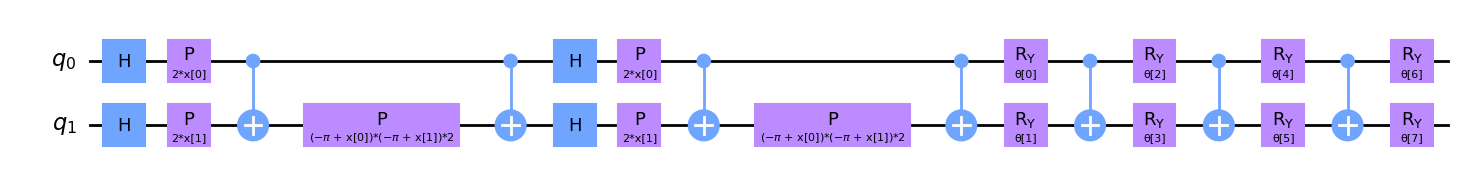
\includegraphics[width=\textwidth]{qiskit_ml_torch_connector_qnn_circuit.png}
    \legend{Fonte: Qiskit Machine Learning \cite{qiskitMachineLearningTorchConnector2026}.}
\end{figure}

Além das codificações utilizadas diretamente em redes neurais quânticas híbridas, existem representações quânticas específicas para imagens, como \textit{Qubit Lattice}, FRQI (\textit{Flexible Representation of Quantum Images}) e NEQR (\textit{Novel Enhanced Quantum Representation}), que buscam codificar coordenadas espaciais e intensidades de pixels por meio de amplitudes, ângulos ou registradores binários. A análise teórica e numérica dessas representações ajuda a evidenciar os limites práticos de medição e escalabilidade ao representar imagens bidimensionais em circuitos quânticos \cite{okada2025measurementlimits}.

\subsection{Modelos variacionais quânticos}

Modelos variacionais quânticos são uma das principais abordagens para uso de computação quântica em dispositivos NISQ. Esses modelos combinam circuitos quânticos parametrizados com otimizadores clássicos. O circuito quântico é responsável por preparar estados, aplicar transformações e produzir medições; o computador clássico calcula a função de custo e atualiza os parâmetros do circuito.

A estrutura geral de um algoritmo variacional pode ser descrita por três componentes: uma função de custo \(C(\theta)\), um circuito parametrizado, também chamado de \textit{ansatz}, e um otimizador clássico. O objetivo é encontrar os parâmetros:

\[
\theta^* =
\arg\min_{\theta}
C(\theta).
\]

A função de custo pode depender de medições realizadas no circuito quântico. Em muitos casos, ela pode ser expressa em termos de valores esperados de observáveis:

\[
C(\theta)
=
\sum_k
f_k
\left(
\operatorname{Tr}
[
O_k U(\theta)\rho_k U^\dagger(\theta)
]
\right),
\]

em que \(O_k\) representa um observável, \(\rho_k\) representa um estado de entrada e \(U(\theta)\) é o circuito parametrizado. Essa formulação mostra como o circuito quântico e o otimizador clássico atuam em conjunto no processo de aprendizagem \cite{cerezo2021variational}.

Em classificação, o circuito pode receber uma entrada codificada \(x\), aplicar uma transformação variacional e produzir saídas por medição. Por exemplo:

\[
z_j(x,\theta)
=
\langle Z_j \rangle
=
\bra{\psi(x,\theta)}
Z_j
\ket{\psi(x,\theta)}.
\]

O vetor \(z(x,\theta)\) pode ser utilizado diretamente para classificação ou enviado a uma camada clássica, como uma camada densa com ativação \textit{softmax}. Assim, o circuito quântico atua como uma camada treinável dentro de um \textit{pipeline} maior. A Figura~\ref{fig:ibm_real_amplitudes} ilustra um circuito do tipo \textit{RealAmplitudes}, composto por camadas alternadas de rotações \(R_Y\) e portas de emaranhamento CNOT, amplamente empregado como \textit{ansatz} variacional em tarefas de aprendizado de máquina quântico.

\begin{figure}[H]
    \centering
    \caption{Circuito \textit{RealAmplitudes} com camadas de rotações \(R_Y\) e portas CNOT, utilizado como exemplo de \textit{ansatz} parametrizado na documentação do Qiskit.}
    \label{fig:ibm_real_amplitudes}
    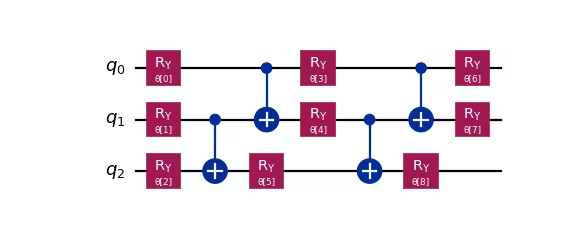
\includegraphics[width=0.78\textwidth]{ibm_real_amplitudes_1.png}
    \legend{Fonte: IBM Quantum \cite{ibmQuantumRealAmplitudes2026}.}
\end{figure}

A escolha do \textit{ansatz} é uma decisão importante. Um \textit{ansatz} muito simples pode não ter capacidade suficiente para representar padrões complexos; por outro lado, um \textit{ansatz} muito profundo pode ser difícil de treinar e mais sensível a ruído. Essa tensão entre expressividade, profundidade, número de qubits e treinabilidade é uma das principais questões em modelos variacionais quânticos.

\subsection{Limitações de simulação, barren plateaus e escalabilidade}

Apesar do potencial dos modelos quânticos, sua aplicação prática ainda enfrenta limitações importantes. A primeira delas é o custo de simulação. Um sistema com \(n\) qubits possui \(2^n\) amplitudes complexas. Assim, a memória necessária para simular exatamente um estado quântico cresce exponencialmente com o número de qubits. Essa limitação é especialmente relevante em pesquisas executadas em computadores clássicos, nas quais o aumento do número de qubits rapidamente se torna inviável.

Outro desafio é a presença de \textit{barren plateaus}. Esse termo descreve regiões da paisagem de otimização nas quais os gradientes da função de custo se tornam muito pequenos. Quando isso ocorre, o otimizador clássico tem dificuldade para encontrar direções úteis de atualização dos parâmetros. \citeonline{mcclean2018barren} demonstraram que, para certas famílias de circuitos quânticos parametrizados, a variância dos gradientes pode decair exponencialmente com o número de qubits.

De forma simplificada, se \(E(\theta)\) representa uma função de custo, o treinamento depende de gradientes como:

\[
\frac{\partial E(\theta)}{\partial \theta_k}.
\]

Em um \textit{barren plateau}, esses gradientes se aproximam de zero para grande parte do espaço de parâmetros:

\[
\frac{\partial E(\theta)}{\partial \theta_k}
\approx 0.
\]

Isso dificulta o treinamento, pois as atualizações de parâmetros tornam-se pouco informativas. Em contraste com redes neurais clássicas, nas quais o desaparecimento do gradiente costuma estar fortemente associado à profundidade da rede, em circuitos quânticos o problema também pode depender fortemente do número de qubits e da forma do \textit{ansatz}.

A escalabilidade também é limitada pelo ruído dos dispositivos NISQ. Circuitos mais profundos tendem a acumular mais erros, e circuitos com muitos qubits exigem maior conectividade e controle físico. Por isso, modelos híbridos atuais costumam utilizar poucos qubits e circuitos relativamente rasos. Essa escolha melhora a viabilidade prática, mas também pode limitar a expressividade do componente quântico.

Em problemas de classificação visual multiclasse, essas limitações exigem redução dimensional prévia por camadas clássicas. Portanto, qualquer comparação entre modelos clássicos e híbridos deve considerar não apenas métricas preditivas, mas também telemetria de tempo de treinamento, estabilidade de convergência, uso de memória e viabilidade de simulação.

\subsection{Simulação de circuitos quânticos e uso do Qiskit}
\label{subsec:simulacao_circuitos_qiskit}

Como os experimentos deste trabalho são conduzidos integralmente em infraestrutura clássica, os circuitos quânticos parametrizados são avaliados por meio de simulação numérica. Essa escolha metodológica garante reprodutibilidade exata e permite construir, depurar e comparar variações de circuitos variacionais ao longo das nove bases de dados sem depender de filas de acesso ou flutuações de calibração de processadores quânticos físicos (QPUs), embora imponha restrições práticas de memória, tempo por época, número de qubits e profundidade de portas.

Ecossistemas como o Qiskit e simuladores de alto desempenho como o Qiskit Aer são fundamentais para estudos experimentais de QML, pois permitem executar circuitos com controle sobre vetores de estado (\textit{statevector}), número de \textit{shots}, cálculo de valores esperados e integração com grafos de diferenciação automática em PyTorch. A documentação da IBM Quantum descreve o uso do Qiskit Aer com primitivas como \textit{Estimator} e \textit{Sampler} \cite{ibmQuantumAerSimulation2026}, enquanto estudos recentes investigam fluxos híbridos quântico-clássicos e aceleração por GPU em simulações quânticas utilizando bibliotecas como NVIDIA Thrust e cuQuantum \cite{bayraktar2023cuquantum,faj2023warpspeed,chen2024quantumhpcworkflow}.

No contexto deste trabalho, ferramentas como Qiskit Aer e bibliotecas de aceleração matricial em GPU atuam na viabilização computacional da simulação clássica dos circuitos quânticos durante o treinamento em lotes, sem alterar a formulação matemática do classificador híbrido. A Figura~\ref{fig:qiskit_aer_cuquantum_workflow} ilustra esse fluxo de execução no Qiskit Aer: o circuito parametrizado é processado pelo transpilador e avaliado pelo simulador de vetor de estado, podendo ser despachado para diferentes \textit{backends} de execução (CPU, GPU com Thrust ou GPU com cuQuantum).

\begin{figure}[H]
    \centering
    \caption{Fluxo de simulação de vetor de estado no Qiskit Aer, incluindo \textit{backends} em CPU, GPU com Thrust e GPU com cuQuantum.}
    \label{fig:qiskit_aer_cuquantum_workflow}
    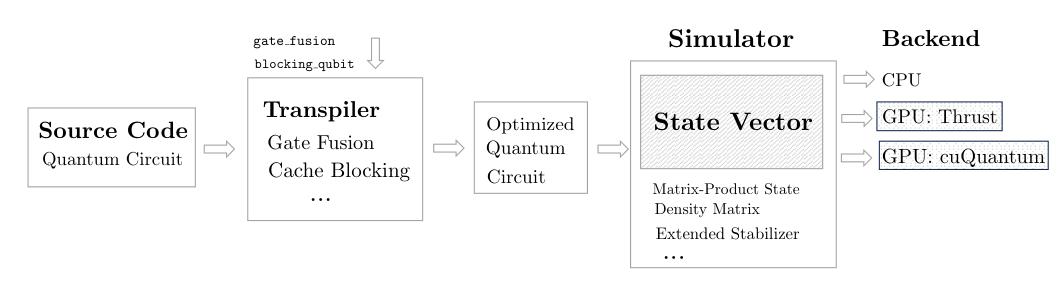
\includegraphics[width=\textwidth]{qiskit_aer_cuquantum_workflow_faj2023.png}
    \legend{Fonte: extraído de Faj et al. \cite{faj2023warpspeed}.}
\end{figure}


\section{Modelos híbridos quântico-clássicos}

Modelos híbridos quântico-clássicos combinam componentes de aprendizado de máquina clássico com circuitos quânticos parametrizados. Essa abordagem é adequada ao cenário NISQ porque permite utilizar circuitos pequenos, enquanto delega ao computador clássico tarefas como pré-processamento, extração de características, otimização e classificação final.

Em tarefas de classificação de imagens, uma estratégia comum é usar uma rede neural clássica, especialmente uma CNN, para extrair características visuais da imagem. Em seguida, essas características são projetadas para uma dimensão compatível com o número de qubits e codificadas em um circuito quântico. O circuito atua como uma camada variacional ou transformadora, e suas saídas são processadas por camadas clássicas responsáveis pela classificação final.

Essa estrutura permite investigar se o componente quântico contribui para a representação dos dados ou para a separação entre classes. No entanto, a simples inclusão de um circuito quântico não garante ganho de desempenho. A contribuição do bloco quântico precisa ser avaliada de forma controlada, comparando-o com \textit{baselines} clássicos equivalentes. Essa integração direta entre redes neurais em PyTorch e módulos quânticos parametrizados é exemplificada na documentação do Qiskit Machine Learning por meio do uso do \textit{TorchConnector} \cite{qiskitMachineLearningTorchConnector2026}.

\subsection{Arquitetura híbrida CNN--circuito quântico}

Em um modelo híbrido para classificação supervisionada de imagens, o fluxo geral de processamento é estruturado em etapas acopladas. A primeira etapa consiste na extração clássica de características espaciais. Considerando um tensor de imagem de entrada \(x \in \mathbb{R}^{H \times W \times C}\) (proveniente de qualquer um dos nove conjuntos de dados do \textit{benchmark}), um extrator convolucional clássico \(g_{\phi}\) produz um vetor de características:

\[
v = g_{\phi}(x),
\]

em que \(\phi\) representa os parâmetros treináveis das camadas convolucionais. Em seguida, esse vetor é projetado linearmente para uma dimensão reduzida \(n\), compatível com o número de qubits do circuito quântico:

\[
u = Wv + b.
\]

\subsection{Camada de codificação clássico-quântica}
\label{subsec:camada_codificacao_classico_quantica}

Na segunda etapa, o vetor latente compacto \(u \in \mathbb{R}^{n}\) é codificado em um registrador quântico inicializado em \(\ket{0}^{\otimes n}\) por meio de um operador unitário de codificação (\textit{feature map} ou \textit{angle embedding}) \(U_{\text{enc}}(u)\), preparando o estado quântico dependente dos dados:

\[
\ket{\psi(u)}
=
U_{\text{enc}}(u)
\ket{0}^{\otimes n}.
\]

\subsection{Camada quântica variacional}
\label{subsec:camada_quantica_variacional}

Na terceira etapa, aplica-se o circuito quântico variacional parametrizado (\textit{ansatz}) \(U(\theta)\), composto por rotações ajustáveis e portas de emaranhamento cujos parâmetros \(\theta\) são otimizados conjuntamente durante o treinamento:

\[
\ket{\psi(u,\theta)}
=
U(\theta)
U_{\text{enc}}(u)
\ket{0}^{\otimes n}.
\]

\subsection{Medição do circuito quântico e retorno ao modelo clássico}
\label{subsec:medicao_retorno_modelo_classico}

Na quarta etapa, a saída do circuito quântico é extraída por meio dos valores esperados de observáveis locais, tipicamente operadores de Pauli-\(Z\) medidos sobre cada um dos \(n\) qubits:

\[
z_j =
\bra{\psi(u,\theta)}
Z_j
\ket{\psi(u,\theta)},
\quad j \in \{1, \dots, n\}.
\]

Esses valores esperados formam um vetor real \(z = [z_1, \dots, z_n]^T \in [-1, 1]^n\), que retorna ao domínio clássico e alimenta a camada linear final de decisão para produzir as probabilidades sobre as \(K\) classes do conjunto de dados:

\[
\hat{y}
=
\operatorname{softmax}(W_c z + b_c).
\]

Essa formulação evidencia que o circuito quântico atua como uma camada intermediária diferenciável dentro de uma arquitetura profunda híbrida. Durante a retropropagação (\textit{backpropagation}), o otimizador clássico ajusta simultaneamente os pesos convolucionais \(\phi\), a projeção de entrada \((W, b)\), os parâmetros quânticos \(\theta\) e a cabeça de classificação \((W_c, b_c)\), minimizando a perda de entropia cruzada categórica associada aos rótulos verdadeiros \cite{schetakis2022qmlframeworks,xiang2024qccnn,long2025qcqcnn,daka2026noqcnn}.

\subsection{CNN com gargalo clássico como baseline de controle}
\label{subsec:cnn_gargalo_baseline}

A utilização de uma variante de CNN com gargalo clássico equivalente como \textit{baseline} de controle metodológico justifica-se pelo fato de a arquitetura híbrida exigir a compressão do vetor de características \(v\) para uma dimensão reduzida \(n\) compatível com o número de qubits simulados. Sem esse controle intermediário, uma eventual diferença de Macro-F1 entre a CNN clássica padrão e o modelo híbrido poderia decorrer exclusivamente do estreitamento dimensional (\textit{bottleneck}), e não das transformações unitárias do circuito quântico. Assim, o gargalo clássico preserva a mesma compactação dimensional \(u \in \mathbb{R}^{n}\), mas substitui o circuito quântico por uma transformação não linear clássica treinável antes da projeção para as \(K\) classes.

\subsection{Comparação com a CNN clássica e abordagens quanvolucionais}
\label{subsec:comparacao_cnn_classica}

A comparação com a CNN clássica depende de compreender as diferentes formas de integração entre operadores convolucionais e circuitos quânticos. A primeira abordagem --- adotada na arquitetura híbrida principal deste estudo --- emprega o extrator convolucional clássico para processar a imagem completa e substitui ou complementa parte das camadas densas finais por um circuito quântico variacional acoplado ao gargalo latente.

Uma segunda abordagem presente na literatura consiste no uso de camadas quanvolucionais (\textit{Quanvolutional Neural Networks}), propostas por \citeonline{henderson2020quanvolutional}. Nessas camadas, pequenas janelas locais da imagem são processadas sequencialmente por circuitos quânticos, de forma análoga à varredura espacial de um filtro convolucional clássico. Dada uma sub-região local \(u_x\) da imagem, aplica-se inicialmente uma função de codificação \(e\):

\[
i_x = e(u_x).
\]

Em seguida, o circuito quântico \(q\) transforma esse estado:

\[
o_x = q(i_x) = q(e(u_x)).
\]

Por fim, uma função de decodificação \(d\), baseada em medições, converte a saída quântica em escalares clássicos que compõem o novo mapa de características:

\[
f_x = d(o_x) = d(q(e(u_x))) = Q(u_x, e, q, d).
\]

Embora as camadas quanvolucionais evitem codificar a imagem inteira em um único circuito largo, sua aplicação em campanhas multi-dataset com dezenas de milhares de imagens impõe um custo proibitivo de simulação, pois o circuito quântico precisa ser executado para cada posição espacial \((i,j)\) de cada imagem em cada época. Por essa razão, na avaliação sistemática dos nove conjuntos de dados deste trabalho, o acoplamento via extração convolucional clássica seguida de projeção para o circuito quântico variacional mostra-se substancialmente mais tratável e escalável, permitindo comparar diretamente desempenho preditivo e telemetria contra a CNN clássica.

\subsection{Limitações práticas de dimensionalidade e custo de simulação em visão computacional}

A aplicação de modelos híbridos quântico-clássicos em conjuntos de dados de visão computacional apresenta desafios estruturais significativos. O primeiro desafio reside na discrepância entre a dimensão de entrada das imagens e o número de qubits viável em simuladores clássicos e dispositivos NISQ atuais. Mesmo imagens compactas de \textit{benchmarks} padronizados possuem entre \(784\) valores de intensidade (em bases \(28 \times 28 \times 1\), como MNIST, Fashion-MNIST, KMNIST e EMNIST) e \(3.072\) valores (em bases RGB \(32 \times 32 \times 3\), como CIFAR-10, CIFAR-100, SVHN e GTSRB), chegando a \(2.304\) valores no FER2013 (\(48 \times 48 \times 1\)). Codificar diretamente milhares de atributos em amplitudes ou rotações individuais de qubits exige circuitos de largura ou profundidade proibitivas para o treinamento iterativo em lotes \cite{okada2025measurementlimits}.

Por conseguinte, arquiteturas híbridas viáveis dependem de um extrator convolucional clássico (\textit{backbone}) para comprimir a imagem original em um vetor latente de baixa dimensão compatível com o número de qubits do circuito variacional, seguido de uma camada clássica de projeção para as \(K\) classes do problema. Essa redução dimensional atua como um gargalo de informação (\textit{information bottleneck}): enquanto em problemas de 10 classes estruturadas a representação comprimida pode reter poder discriminativo suficiente, em problemas com maior cardinalidade ou granularidade semântica (como CIFAR-100 Coarse com 20 superclasses heterogêneas, GTSRB com 43 classes ou EMNIST Balanced com 47 classes) ou alta sobreposição visual (como FER2013), o gargalo quântico pode limitar a capacidade de separação do modelo. Além disso, o cálculo de gradientes quânticos (como via regra de deslocamento de parâmetros ou diferenciação adjunta em simuladores de vetor de estado) impõe um custo computacional por época substancialmente superior ao de camadas densas clássicas, tornando indispensável a medição conjunta de métricas preditivas e telemetria de tempo de execução \cite{faj2023warpspeed,chen2024quantumhpcworkflow}.

\section{Trabalhos correlatos}
\label{sec:trabalhos_correlatos}

Esta seção apresenta os estudos empíricos correlatos identificados para cada uma das nove bases de dados que compõem o \textit{benchmark} deste TCC. Seguindo a diretriz metodológica estabelecida na Seção~2.1, analisam-se primeiramente os trabalhos baseados em arquiteturas clássicas de redes neurais convolucionais e, em seguida, os estudos que propõem modelos quânticos e híbridos quântico-clássicos. Dentro de cada grupo, a exposição obedece rigorosamente à mesma sequência dos nove conjuntos de dados: MNIST, Fashion-MNIST, KMNIST, EMNIST Balanced, CIFAR-10, CIFAR-100 Coarse, SVHN, GTSRB e FER2013.

Cumpre destacar que todos os valores numéricos relatados nesta seção pertencem exclusivamente aos autores das respectivas publicações e devem ser interpretados dentro das condições de cada artigo (partição avaliada, número de classes, pré-processamento e métrica adotada). Em particular, acurácias publicadas na literatura não são diretamente equivalentes ao Macro-F1 empregado neste TCC, nem resultados obtidos em recortes binários ou de quatro classes podem ser equiparados, sem qualificação explícita, a tarefas de 10, 20, 43 ou 47 classes. Os resultados próprios obtidos na campanha experimental deste projeto são apresentados separadamente no Capítulo~\ref{cap:resultados}.

\subsection{Estudos com arquiteturas clássicas nos nove conjuntos de dados}
\label{subsec:correlatos_classicos}

A Tabela~\ref{tab:correlatos_classicos_9_bases} sintetiza as arquiteturas clássicas analisadas ao longo das nove bases de dados, detalhando o método de treinamento, o resultado relatado pelos autores e as condições ou ressalvas de protocolo identificadas na conferência das fontes primárias.

\begin{table}[htb]
\centering
\caption{Síntese dos estudos correlatos com arquiteturas clássicas nos nove conjuntos de dados do \textit{benchmark}.}
\label{tab:correlatos_classicos_9_bases}
\resizebox{\textwidth}{!}{%
\begin{tabular}{p{2.9cm}p{6.8cm}p{8.2cm}}
\toprule
\textbf{Dataset} & \textbf{Artigo, arquitetura e método} & \textbf{Resultado relatado pelos autores e condição de protocolo} \\
\midrule
\textbf{MNIST} & \citeonline{kabir2023spinalnet} (SpinalNet): VGG-5 com conexões totalmente conectadas graduais (\textit{Spinal FC}); 100 épocas. & 99,69\% de acurácia média de teste (melhor: 99,72\%). A VGG-5 padrão sem \textit{Spinal FC} atingiu os mesmos valores nessa configuração. \\
\textbf{Fashion-MNIST} & \citeonline{khanday2021filter}: CNN com duas convoluções (32 filtros), comparando \textit{kernels} \(3 \times 3\), \(5 \times 5\) e \(7 \times 7\); otimizador Adam. & Para filtro \(3 \times 3\), a tabela original informa \textbf{92,68\% em teste} e 92,35\% em validação (o resumo cita 93,68\%, divergindo da tabela e da conclusão). \\
\textbf{KMNIST} & \citeonline{kabir2023spinalnet} (SpinalNet): VGG-5 + \textit{Spinal FC}, 10 classes; treinamento por 200 épocas. & 99,05\% de acurácia média de teste e 99,15\% no melhor resultado (não se deve confundir o máximo com a média). \\
\textbf{EMNIST Balanced} & \citeonline{kabir2023spinalnet}: VGG-5 + \textit{Spinal FC}, 47 classes, 200 épocas. \citeonline{chen2023handwritten}: compara CNN proposta e LeNet-5. & \citeonline{kabir2023spinalnet}: 90,73\% de acurácia média de teste (melhor: 91,05\%). \citeonline{chen2023handwritten}: 89,36\% em \textbf{validação}, e não em teste. \\
\textbf{CIFAR-10} & \citeonline{khanday2021filter}: CNN com filtros \(3 \times 3\) e 50 épocas; Adam. & Tabela 1 do artigo: 94,26\% no treino, 72,75\% na validação e \textbf{73,04\% no teste} (há equívoco no texto corrido que menciona 63,5\%). \\
\textbf{CIFAR-100 Coarse} & \citeonline{guo2018cnnrnn}: arquitetura hierárquica CNN-RNN com \textit{Wider-ResNet}, prevendo simultaneamente 100 classes finas e 20 superclasses; aumento de dados. & \textbf{88,23\%} de acurácia nas 20 superclasses, contra 85,38\% da rede treinada apenas para \textit{coarse}. Tarefa conjunta e capacidade arquitetural diferem do TCC. \\
\textbf{SVHN} & \citeonline{huang2017densenet} (DenseNet): conexões densas; variante DenseNet de 100 camadas e taxa de crescimento \(k=24\). & 1,59\% de erro de teste na configuração relatada (\(\approx 98{,}41\%\) de acurácia); requer considerar o pré-processamento e o uso do conjunto extra de treino. \\
\textbf{GTSRB} & \citeonline{an2024lenet5gtsrb}: LeNet-5 modificada, pré-processamento dedicado, alterações de \textit{pooling} e ativação PReLU. & 97,53\% de acurácia relatada (partição de 31.433 treino, 7.776 validação e 12.630 teste); requer atenção ao agrupamento por sequência (\textit{track}). \\
\textbf{FER2013} & \citeonline{li2021autofernet} (Auto-FERNet): arquitetura leve via busca diferenciável de arquitetura e re-rotulagem (\textit{relabeling}) por similaridade. & 73,78\% de acurácia de teste sem \textit{ensemble} nem dados externos, segundo o resumo dos autores; depende das regras aplicadas no \textit{relabeling}. \\
\bottomrule
\end{tabular}%
}
\legend{Fonte: Elaborado pelo autor (2026), a partir da auditoria das publicações originais.}
\end{table}

Nas bases monocromáticas de \(28 \times 28\) pixels com 10 classes, observa-se elevada maturidade das arquiteturas convolucionais clássicas, mas também diferenças importantes de protocolo. No \textbf{MNIST}, \citeonline{kabir2023spinalnet} propõem a arquitetura SpinalNet, na qual as camadas densas finais recebem entradas de forma gradual e repetida (\textit{Spinal FC}) acopladas a um extrator VGG-5 treinado por 100 épocas. Os autores relatam 99,69\% de acurácia média de teste e 99,72\% na melhor execução; contudo, na tabela comparativa do próprio estudo, o \textit{baseline} VGG-5 padrão sem \textit{Spinal FC} alcança exatamente os mesmos patamares nessa base, evidenciando que a extração convolucional já satura a separabilidade dos dígitos. No \textbf{Fashion-MNIST}, \citeonline{khanday2021filter} avaliam uma CNN rasa composta por duas camadas convolucionais de 32 filtros otimizada com Adam, variando o tamanho dos núcleos (\(3 \times 3\), \(5 \times 5\) e \(7 \times 7\)). Para o filtro \(3 \times 3\), a tabela de resultados do artigo registra 92,68\% de acurácia no conjunto de teste e 92,35\% na validação; registra-se, como cuidado de auditoria bibliográfica, que o resumo daquela publicação menciona 93,68\%, valor em desacordo com a tabela e com a conclusão do próprio texto. Outros trabalhos levantados na amostra para o Fashion-MNIST exploram combinações de múltiplas CNNs \cite{nocentini2022fashionmnist} e revisões de estado da arte com arquiteturas pesadas e aumento intensivo de dados \cite{mukhamediev2024fashionmnist}, cujas configurações extrapolam o regime de controle leve adotado neste TCC.

No \textbf{KMNIST}, introduzido por \citeonline{clanuwat2018kmnist} para caracteres cursivos Kuzushiji, \citeonline{kabir2023spinalnet} aplicam o modelo VGG-5 com cabeçalho \textit{Spinal FC} ao longo de 200 épocas, obtendo 99,05\% de acurácia média de teste e 99,15\% no melhor resultado individual --- distinção relevante para evitar a comparação indevida entre valores máximos isolados e médias de execução. Na extensão alfanumérica \textbf{EMNIST Balanced} (47 classes), o mesmo protocolo de \citeonline{kabir2023spinalnet} atinge 90,73\% de acurácia média de teste (melhor resultado de 91,05\%), refletindo o aumento de dificuldade imposto pela multiplicação de categorias e pela ambiguidade visual entre letras e números. Ainda sobre o EMNIST Balanced, \citeonline{chen2023handwritten} compara uma CNN customizada contra a arquitetura clássica LeNet-5 e reporta 89,36\% de acurácia; todavia, a conferência do artigo mostra que esse número corresponde ao conjunto de \textbf{validação}, e não ao conjunto de teste independente. Trabalhos adicionais como o de \citeonline{abosamra2021optimized} empregam blocos residuais concatenados em profundidade para classificação de caracteres manuscritos, reforçando a sensibilidade do domínio ao desenho do extrator espacial.

Passando às bases coloridas (RGB) de objetos naturais em resolução \(32 \times 32\), \citeonline{khanday2021filter} avaliam sua CNN de filtros \(3 \times 3\) no \textbf{CIFAR-10} por 50 épocas, reportando na Tabela~1 do artigo 94,26\% de acurácia de treinamento, 72,75\% de validação e 73,04\% de teste (observando-se que um parágrafo do texto original menciona 63,5\% por erro tipográfico ao referir-se ao filtro \(3 \times 3\)). A expressiva diferença entre treino (94,26\%) e teste (73,04\%) em uma CNN simples sem regularização pesada ilustra a tendência ao sobreajuste no CIFAR-10, motivo pelo qual estudos clássicos de alto desempenho recorrem a conexões residuais \cite{he2016resnet}, busca diferenciável de arquitetura como no ajuste fino de DARTS \cite{tanveer2021darts} ou políticas aprendidas de aumento de dados como o AutoAugment \cite{cubuk2019autoaugment}. Já para o \textbf{CIFAR-100 Coarse} (20 superclasses), incluiu-se como referência específica o trabalho de \citeonline{guo2018cnnrnn}, que propõe uma arquitetura hierárquica CNN-RNN baseada em \textit{Wider-ResNet} com aumento de dados para prever conjuntamente os 100 rótulos finos e as 20 superclasses. Nessa configuração multitarefa, os autores relatam 88,23\% de acurácia nas 20 superclasses, superando os 85,38\% obtidos pela mesma rede treinada exclusivamente para o nível \textit{coarse}. Embora anterior ao recorte principal de busca, o estudo de \citeonline{guo2018cnnrnn} justifica-se por reportar explicitamente o desempenho nas 20 superclasses oficiais, devendo-se ressalvar que sua profundidade arquitetural e a supervisão conjunta fina--grossa diferem substancialmente de uma CNN treinada apenas com os rótulos de superclasse.

Nos domínios de cenas reais e forte desbalanceamento, \citeonline{huang2017densenet} estabeleceram uma referência seminal no \textbf{SVHN} por meio das redes densamente conectadas (DenseNet), nas quais cada camada recebe mapas de características de todas as camadas precedentes. Na configuração DenseNet de 100 camadas e fator de crescimento \(k=24\), os autores reportam taxa de erro de teste de 1,59\% (equivalente a aproximadamente 98,41\% de acurácia), protocolo que usualmente incorpora o conjunto extra de treinamento do SVHN (mais de 530 mil imagens adicionais), diferenciando-se de campanhas restritas à partição base. Para o reconhecimento de placas de trânsito no \textbf{GTSRB} (43 classes), \citeonline{an2024lenet5gtsrb} propõem uma versão leve e aprimorada da LeNet-5 combinando pré-processamento de imagem, reformulação das camadas de \textit{pooling} e função de ativação PReLU, relatando 97,53\% de acurácia sobre uma divisão de 31.433 imagens de treino, 7.776 de validação e 12.630 de teste; na mesma linha de redes leves para sinalização viária, \citeonline{wei2024lightweightgtsrb} exploram extração multiescala e mecanismos de atenção. Por fim, no reconhecimento de expressões faciais no \textbf{FER2013} (7 classes), \citeonline{li2021autofernet} apresentam a Auto-FERNet, obtida por busca diferenciável de arquitetura aliada a uma estratégia de re-rotulagem (\textit{relabeling}) baseada em similaridade para mitigar rótulos ruidosos, relatando 73,78\% de acurácia de teste sem uso de \textit{ensembles} ou bases externas.

\subsection{Estudos com arquiteturas quânticas e híbridas nos nove conjuntos de dados}
\label{subsec:correlatos_quanticos}

Na sequência, a Tabela~\ref{tab:correlatos_quanticos_9_bases} organiza os estudos correlatos que empregam circuitos quânticos variacionais, filtros quanvolucionais ou redes híbridas quântico-clássicas ao longo das mesmas nove bases de dados, destacando os resultados reportados e as restrições metodológicas de cada experimento.

\begin{table}[htb]
\centering
\caption{Síntese dos estudos correlatos com arquiteturas quânticas e híbridas nos nove conjuntos de dados do \textit{benchmark}.}
\label{tab:correlatos_quanticos_9_bases}
\resizebox{\textwidth}{!}{%
\begin{tabular}{p{2.9cm}p{6.8cm}p{8.2cm}}
\toprule
\textbf{Dataset} & \textbf{Artigo, arquitetura e método quântico/híbrido} & \textbf{Resultado relatado pelos autores e restrições de protocolo} \\
\midrule
\textbf{MNIST} & \citeonline{riaz2023nnqe} (NNQE): filtro quântico fixo com emaranhamento seguido de camada densa (PennyLane). \citeonline{long2025qcqcnn} (QCQ-CNN): filtro quântico fixo + CNN rasa + classificador variacional de 2 qubits. & \citeonline{riaz2023nnqe} (10 classes): 93,8\% em teste e 95,1\% em treino (vs. 92,0\% e 93,5\% na rede clássica). \citeonline{long2025qcqcnn} (tarefa \textbf{binária} 3 vs. 5): \(98{,}85 \pm 0{,}25\%\) (vs. \(98{,}79 \pm 0{,}13\%\) na CNN), com lotes distintos (1 vs. 4). \\
\textbf{Fashion-MNIST} & \citeonline{bokhan2022qcnn}: QCNN variacional em Cirq/TFQ (50 épocas). \citeonline{song2024resourceefficient}: filtros quânticos QAOA de 5 qubits. \citeonline{long2025qcqcnn}: QCQ-CNN. & \citeonline{bokhan2022qcnn} (4 classes 0/1/2/3): 85,93\% vs. CNN 89,69\%. \citeonline{song2024resourceefficient} (10 classes): média de 92,59\% em 5 inicializações (verificar partição da curva). \citeonline{long2025qcqcnn} (\textbf{binário} camiseta/calça): \(99{,}41 \pm 0{,}14\%\). \\
\textbf{KMNIST} & \citeonline{dong2025weightremapping}: CNN híbrida baseada em remapeamento de pesos (\textit{weight remapping}). & O resumo confirma experimento \textbf{binário} em KMNIST; o valor numérico exato e o protocolo integral dependem de verificação no texto completo. \\
\textbf{EMNIST} & \citeonline{riaz2026emnist}: filtro quântico fixo de 4 qubits com rotações e duas portas CNOT antes de rede totalmente conectada. & 75,9\% em teste vs. 68,9\% sem filtro quântico, em 47 classes. O texto mistura os nomes \textit{Balanced} e \textit{ByMerge}, embora use as contagens 112.800/18.800 de \textit{Balanced}. \\
\textbf{CIFAR-10} & \citeonline{riaz2023nnqe} (NNQE). \citeonline{kong2026cqnas} (CQNAS): CNN combinada à busca de arquitetura de circuitos variacionais. & \citeonline{riaz2023nnqe}: 36,0\% em teste e 42,0\% em treino (vs. 30,5\% e 34,1\% na rede clássica simples). \citeonline{kong2026cqnas}: divulga 95,44\% de acurácia (requer conferência de partição e \textit{backbone} no texto integral). \\
\textbf{CIFAR-100 Coarse} & Não foi identificado estudo quântico/híbrido confirmado para as \textbf{20 superclasses oficiais} (\textit{coarse}). & Estudos em CIFAR-100 com 100 classes, recortes binários ou agrupamentos próprios dos autores não equivalem ao protocolo de 20 superclasses; mantido como lacuna aberta. \\
\textbf{SVHN} & \citeonline{kong2026cqnas} (CQNAS): rede convolucional acoplada a circuitos variacionais com busca de arquitetura. & O resumo confirma a avaliação na base SVHN, mas o resultado específico e o protocolo de particionamento exigem extração do texto integral. \\
\textbf{GTSRB} & \citeonline{riaz2023nnqe} (NNQE): filtro quântico fixo com emaranhamento seguido de rede densa (43 classes). & Teste: \textbf{73,4\%} no NNQE vs. \textbf{82,2\%} na rede clássica (treino: 97,5\% vs. 96,2\%). Evidencia que a abordagem híbrida não melhora todas as tarefas e exibe sobreajuste. \\
\textbf{FER2013} & \citeonline{alsubai2024quantumfer}: ResNet-18 combinada a mecanismo híbrido proposto para 7 expressões faciais. & Relata 98,19\% de acurácia, mas a soma da tabela de classes difere em 10 imagens do total canônico (35.887) e o protocolo requer auditoria; não usar como comparação conclusiva. \\
\bottomrule
\end{tabular}%
}
\legend{Fonte: Elaborado pelo autor (2026), a partir da auditoria das publicações originais.}
\end{table}

A análise detalhada da literatura quântica e híbrida revela contrastes metodológicos fundamentais em relação aos modelos clássicos. No \textbf{MNIST}, \citeonline{riaz2023nnqe} propõem o modelo NNQE (\textit{Neural Network with Quantum Entanglement}), que aplica um filtro quântico fixo não treinável com portas de emaranhamento sobre janelas locais da imagem antes de uma camada totalmente conectada clássica, simulado no PennyLane. Na tarefa completa de 10 classes do MNIST, o NNQE alcança 93,8\% de acurácia de teste e 95,1\% de treino, superando a rede densa clássica de referência do próprio artigo (92,0\% em teste e 93,5\% em treino), mas permanecendo substancialmente abaixo de CNNs clássicas completas (que superam 99\%). Por sua vez, \citeonline{long2025qcqcnn} avaliam a arquitetura QCQ-CNN (composta por filtro quanvolucional fixo, CNN clássica rasa e classificador variacional treinável de 2 qubits) na tarefa estritamente \textbf{binária} de separação entre os dígitos 3 e 5 do MNIST. Em dez execuções independentes (até 100 épocas, otimizador Adam e parada antecipada), a Tabela~1 daquele estudo reporta \(98{,}85 \pm 0{,}25\%\) para a QCQ-CNN contra \(98{,}79 \pm 0{,}13\%\) para a CNN clássica; contudo, além de o experimento restringir-se a duas classes e de a tabela não explicitar textualmente a partição do número reportado, o tamanho do lote foi configurado como \textit{batch size} 1 na QCQ-CNN e \textit{batch size} 4 nos modelos clássicos e QCCNN, introduzindo um fator de confusão no regime de atualização de gradientes. Ainda no MNIST, \citeonline{bokhan2022qcnn} (cuja leitura deve ser acompanhada de sua corrigenda \cite{bokhan2022corrigendum}) avaliam uma QCNN variacional restrita a quatro classes (dígitos 3, 4, 5 e 6), obtendo 85,14\% de acurácia contra 94,25\% da CNN clássica de comparação. Outros trabalhos metodológicos recentes investigam mecanismos de autoatenção com kernel quântico (QKSAN e QSAN) \cite{zhao2024qksan,shi2025qsan} e codificação em qubit único \cite{easommccaldin2024singlequbit} em subconjuntos de dígitos, além do trabalho conceitual pioneiro sobre camadas quanvolucionais de \citeonline{henderson2020quanvolutional}, que introduziu filtros quânticos aleatórios como extratores locais sem cabeça variacional treinável.

No \textbf{Fashion-MNIST}, repetem-se recortes com número reduzido de categorias ou configurações específicas de filtragem. \citeonline{bokhan2022qcnn,bokhan2022corrigendum} treinam uma QCNN variacional em Cirq/TensorFlow Quantum por 50 épocas sobre apenas quatro classes (0, 1, 2 e 3), relatando 85,93\% de acurácia para o modelo quântico frente a 89,69\% da CNN clássica. Na tarefa binária (camiseta vs. calça), \citeonline{long2025qcqcnn} reportam \(99{,}41 \pm 0{,}14\%\) para a QCQ-CNN contra \(99{,}19 \pm 0{,}19\%\) para a CNN sob a mesma assimetria de tamanho de lote mencionada anteriormente. Já na formulação completa de 10 classes do Fashion-MNIST, \citeonline{song2024resourceefficient} propõem uma QCNN eficiente em recursos baseada em filtros quânticos inspirados em QAOA de 5 qubits e relatam acurácia média de 92,59\% em cinco inicializações aleatórias; todavia, a análise cuidadosa da publicação exige verificar na figura correspondente qual partição sustenta a curva apresentada antes de tratá-la como acurácia de teste padronizada.

Para o \textbf{KMNIST}, o estudo de \citeonline{dong2025weightremapping} propõe uma rede neural híbrida baseada em remapeamento de pesos (\textit{weight remapping}); entretanto, a conferência do resumo confirma que o experimento conduzido na base Kuzushiji restringe-se a uma tarefa \textbf{binária}, permanecendo pendente a verificação no texto integral quanto a eventuais testes nas 10 classes originais. No \textbf{EMNIST}, \citeonline{riaz2026emnist} empregam um filtro quântico fixo de 4 qubits (composto por rotações angulares e duas portas CNOT) acoplado a uma rede totalmente conectada para classificar 47 categorias, relatando ganho de 68,9\% (rede sem filtro quântico) para 75,9\% (com filtro quântico) no conjunto de teste. Ao analisar esse artigo, identificou-se uma ambiguidade importante de rotulagem: os autores alternam no texto as denominações \textit{EMNIST Balanced} e \textit{EMNIST ByMerge}, embora os volumes informados (112.800 amostras de treino e 18.800 de teste, em 47 classes) correspondam exatamente à partição oficial \textit{Balanced}. Essa observação reforça a necessidade de auditar as contagens amostrais em vez de confiar apenas na nomenclatura declarada.

Nos conjuntos RGB de imagens naturais e urbanas, as limitações de compressão e generalização dos modelos híbridos tornam-se mais visíveis. No \textbf{CIFAR-10}, o modelo NNQE de \citeonline{riaz2023nnqe} obtém apenas 36,0\% de acurácia de teste e 42,0\% de treino nas 10 classes (contra 30,5\% e 34,1\% de sua linha de base clássica sem convoluções profundas), refletindo a insuficiência de uma camada densa precedida por filtro quântico fixo para capturar texturas coloridas complexas. Em contrapartida, \citeonline{kong2026cqnas} propõem o arcabouço CQNAS (\textit{Collaborative Quantum Neural Architecture Search}), que combina redes convolucionais clássicas e busca automatizada de circuitos variacionais, divulgando no resumo 95,44\% de acurácia no CIFAR-10 e aplicação adicional na base \textbf{SVHN}; contudo, como os detalhes do particionamento, do peso relativo do \textit{backbone} clássico e do resultado numérico exato em SVHN dependem da leitura integral do artigo, esses valores não devem ser interpretados isoladamente como ganho puramente quântico. Já para o \textbf{CIFAR-100 Coarse}, não foi encontrado, em todo o material auditado, nenhum estudo quântico ou híbrido que reporte resultados confirmados especificamente nas \textbf{20 superclasses oficiais}: trabalhos que mencionam CIFAR-100 em tarefas binárias, subconjuntos ad hoc de poucas classes ou na formulação de 100 classes finas não atendem ao recorte de 20 superclasses, configurando uma lacuna empírica direta na literatura revisada.

No \textbf{GTSRB} (43 classes), os resultados de \citeonline{riaz2023nnqe} oferecem um contraexemplo empírico fundamental contra afirmações genéricas de superioridade quântica: enquanto no conjunto de treinamento o modelo híbrido NNQE atingiu 97,5\% de acurácia (contra 96,2\% da rede clássica de referência), no conjunto de teste o desempenho do NNQE caiu para \textbf{73,4\%}, ficando 8,8 pontos percentuais abaixo da rede clássica (\textbf{82,2\%}). Esse descompasso acentuado entre treino e teste demonstra que a transformação quântica fixa não impediu o sobreajuste e degradou a generalização frente às 43 classes desbalanceadas de placas de trânsito. No \textbf{FER2013} (7 expressões faciais), identificou-se como candidato recente o trabalho de \citeonline{alsubai2024quantumfer}, que integra uma arquitetura ResNet-18 a um mecanismo híbrido quântico-clássico e relata 98,19\% de acurácia; todavia, a conferência preliminar constatou que a soma das amostras na tabela de distribuição de classes daquele artigo difere em 10 imagens do total canônico de 35.887 exemplos do FER2013 e que um valor acima de 98\% destoa drasticamente dos \textit{benchmarks} consolidados da literatura na base original (situados na faixa de 70\% a 75\%, como em \citeonline{li2021autofernet}), exigindo auditoria estrita de vazamento ou filtragem de dados antes de qualquer comparação. Por fim, cabe mencionar que o trabalho de \citeonline{daka2026noqcnn} (No-QCNN), embora já citado na fundamentação por discutir circuitos convolucionais quânticos sem \textit{pooling} em simulador Qiskit, avalia seu modelo exclusivamente sobre um conjunto sintético próprio de 50 imagens de linhas coloridas em 6 classes (relatando 82,05\% de acurácia de validação), não constituindo, portanto, resultado empírico em nenhuma das nove bases do TCC.

\section{Síntese da lacuna de pesquisa}
\label{sec:lacuna_pesquisa}

A análise conjunta dos estudos clássicos e quântico-clássicos revisados nas Seções~\ref{subsec:correlatos_classicos} e~\ref{subsec:correlatos_quanticos} permite formular a lacuna de pesquisa de maneira estritamente proporcional à evidência examinada:
\begin{enumerate}
    \item \textbf{Fragmentação de protocolos e recortes de classes na literatura híbrida}: no conjunto de trabalhos quânticos e híbridos levantados, predominam avaliações restritas a recortes binários (como MNIST 3 vs. 5 e Fashion-MNIST de 2 classes em \citeonline{long2025qcqcnn}, ou KMNIST binário em \citeonline{dong2025weightremapping}), subconjuntos de 4 classes \cite{bokhan2022qcnn}, conjuntos sintéticos reduzidos \cite{daka2026noqcnn} ou arquiteturas com filtros quânticos fixos não treináveis seguidos apenas de camadas densas \cite{riaz2023nnqe,riaz2026emnist}, além da ausência confirmada de resultados quânticos para as 20 superclasses oficiais do CIFAR-100 Coarse;
    \item \textbf{Heterogeneidade de métricas e omissão do Macro-F1}: os artigos revisados reportam quase exclusivamente a acurácia global (por vezes sobre o conjunto de validação, como em \citeonline{chen2023handwritten}, ou com divergências internas entre resumo e tabelas, como em \citeonline{khanday2021filter}), métrica que não pondera igualmente categorias minoritárias em bases severamente desbalanceadas como GTSRB, FER2013 e SVHN;
    \item \textbf{Variáveis de confusão nas comparações entre modelos}: mesmo quando um artigo compara modelos clássicos e híbridos, frequentemente ocorrem diferenças de tamanho de lote (como lote 1 vs. lote 4 em \citeonline{long2025qcqcnn}), ausência de um controle clássico com gargalo dimensional equivalente (\textit{bottleneck}) ou falta de detalhamento sobre a topologia exata dos circuitos acoplados e o tempo de simulação.
\end{enumerate}

Diante dessas constatações, este trabalho contribui ao executar e documentar uma campanha experimental padronizada sobre as nove bases de dados completas (MNIST, Fashion-MNIST, KMNIST, EMNIST Balanced, CIFAR-10, CIFAR-100 Coarse, SVHN, GTSRB e FER2013), avaliada prioritariamente por Macro-F1 e acompanhada de controle vetorial de gargalo (\texttt{Dense20}), explicitação das configurações de treinamento e registro transparente das limitações de particionamento e simulação, conforme descrito nos Capítulos~\ref{cap:desenvolvimento} e~\ref{cap:resultados}.


% ---------------------------------------------------------------
% CAPÍTULO 3 - DESENVOLVIMENTO / PROPOSTA METODOLÓGICA
% ---------------------------------------------------------------
\chapter{Desenvolvimento}
\label{cap:desenvolvimento}

Este trabalho caracteriza-se como uma \textbf{pesquisa aplicada}, de abordagem predominantemente \textbf{quantitativa} e objetivos \textbf{exploratórios, descritivos e comparativos}. Seu desenvolvimento combina pesquisa bibliográfica com experimentos computacionais de classificação supervisionada de imagens. A revisão identifica trabalhos de aprendizado profundo clássico e de modelos híbridos quântico-clássicos nos conjuntos de dados selecionados. Os experimentos avaliam configurações de referência e híbridas em bases públicas, por meio de métricas preditivas e de custo computacional, conforme as partições e condições descritas neste capítulo. As operações quânticas são avaliadas por simulação, e os resultados obtidos são interpretados considerando as diferenças entre arquiteturas, partições e protocolos.

Cabe explicitar que caracterizar o desenho experimental como comparativo não significa assumir que todas as configurações diferem por um único fator isolado. Ao longo deste capítulo, detalham-se, para cada contraste avaliado, quais componentes são efetivamente compartilhados (como as partições de dados, o redimensionamento espacial e o extrator convolucional base) e quais elementos diferem entre as configurações (incluindo transformações intermediárias, quantidade de parâmetros treináveis, estrutura da cabeça de saída e sementes de otimização). Além disso, descreve-se como executado exclusivamente aquilo que consta nos artefatos da campanha auditada em 30/10/2026, apresentando-se extensões adicionais como propostas para trabalhos futuros.

\section{Solução proposta}
\label{sec:solucao}

A solução desenvolvida consiste em um \textit{pipeline} computacional unificado e auditável para classificação supervisionada multiclasse nos nove conjuntos de dados do \textit{benchmark} (MNIST, Fashion-MNIST, KMNIST, EMNIST Balanced, CIFAR-10, CIFAR-100 Coarse, SVHN, GTSRB e FER2013). Esse \textit{pipeline} abrange o inventário e padronização das bases de dados, o pré-processamento e redimensionamento dos tensores de imagem, a separação em subconjuntos de treino, validação e teste, a implementação modular das arquiteturas clássicas e híbrida, a execução das campanhas de treinamento e a consolidação das métricas preditivas e de telemetria.

Na campanha experimental auditada em 30/10/2026, que totalizou \textbf{72 \textit{checkpoints}} (oito configurações por conjunto de dados ao longo das nove bases, com uma semente de otimização registrada para cada configuração), a comparação arquitetural estruturou-se em torno de três famílias principais de modelos, complementadas por variações clássicas de ativação, tamanho de lote e quantização:
\begin{enumerate}
    \item \textbf{CNN clássica original (\textit{baseline})}: arquitetura convolucional responsável pela extração hierárquica de características e classificação direta nas \(K\) classes de cada conjunto de dados, servindo também de base para as análises de funções de ativação, tamanho de lote (\textit{batch size}) e quantização pós-treinamento;
    \item \textbf{CNN com gargalo vetorial clássico de 20 dimensões (\texttt{Dense20})}: variante de controle experimental que projeta as características extraídas pelo \textit{backbone} para um vetor latente de \(n=20\) dimensões antes da camada linear de decisão, permitindo avaliar o efeito da compactação dimensional no domínio puramente clássico;
    \item \textbf{Arquitetura híbrida quântico-clássica (\texttt{Híbrido Mac/PennyLane})}: composta pelo extrator convolucional clássico acoplado a uma cabeça híbrida formada por \textbf{quatro circuitos quânticos variacionais independentes de cinco qubits cada} (totalizando 20 entradas angulares distribuídas em 4 subcircuitos de 5 qubits simulados em PennyLane, e não um único circuito emaranhado de 20 qubits), seguida da projeção linear final para as \(K\) categorias.
\end{enumerate}

A pergunta de pesquisa que orienta o desenvolvimento pode ser sintetizada da seguinte forma: \textit{em tarefas de classificação supervisionada de imagens ao longo das nove bases do benchmark (MNIST, Fashion-MNIST, KMNIST, EMNIST Balanced, CIFAR-10, CIFAR-100 Coarse, SVHN, GTSRB e FER2013), como se comporta o desempenho em Macro-F1 da arquitetura híbrida baseada em quatro circuitos independentes de 5 qubits em comparação à CNN clássica original e ao controle vetorial \texttt{Dense20} sob as mesmas partições experimentais, e quais limites de generalização, custo computacional e protocolo emergem dessa avaliação?}

\section{Tipo de pesquisa e escopo metodológico}

Do ponto de vista metodológico, a natureza aplicada do trabalho decorre do desenvolvimento e avaliação empírica de um procedimento concreto para classificação supervisionada de imagens em múltiplos domínios. A abordagem quantitativa fundamenta-se na mensuração de indicadores preditivos (prioritariamente o Macro-F1 no conjunto de teste, acompanhado de acurácia, precisão, revocação, matrizes de confusão e variações por classe \(\Delta\text{F1}\)) e de indicadores operacionais (tempo de execução, \textit{throughput}, latência e recursos de simulação). Os objetivos são simultaneamente exploratórios (ao investigar o comportamento de cabeças quânticas simuladas em bases pouco exploradas na literatura, como CIFAR-100 Coarse e EMNIST Balanced), descritivos (ao documentar sistematicamente métricas, hiperparâmetros e artefatos dos 72 \textit{checkpoints}) e comparativos (ao contrastar as configurações avaliadas sob as mesmas divisões amostrais).

\section{Visão geral da solução proposta}
\label{subsec:visao_arquitetura}

A arquitetura geral do \textit{pipeline} experimental organiza-se em seis etapas sequenciais e integradas:
\begin{enumerate}
    \item \textbf{Inventário e padronização das 9 bases de dados}: carregamento automatizado e verificação de integridade dos conjuntos MNIST, Fashion-MNIST, KMNIST, EMNIST Balanced, CIFAR-10, CIFAR-100 Coarse, SVHN, GTSRB e FER2013 a partir das especificações centralizadas em \path{configs/datasets.yaml};
    \item \textbf{Pré-processamento e particionamento}: conversão para tensores numéricos, normalização de intensidade por canal, redimensionamento espacial padronizado (para \(64 \times 64\) pixels na maioria das bases e \(128 \times 128\) pixels no GTSRB na campanha auditada) e separação nos subconjuntos de treino, validação e teste registrados na Tabela~\ref{tab:caracterizacao_9_datasets};
    \item \textbf{Campanha experimental da CNN clássica}: treinamento e avaliação das configurações clássicas ao longo das nove bases, contemplando o \textit{baseline} original e variações controladas de funções de ativação, tamanhos de lote e quantização;
    \item \textbf{Controle de redução dimensional (\texttt{Dense20})}: avaliação do modelo clássico com camada densa intermediária de 20 unidades para contrastar diretamente com a dimensão total de entrada da cabeça híbrida;
    \item \textbf{Campanha experimental do modelo híbrido quântico-clássico}: acoplamento do extrator convolucional aos quatro circuitos variacionais independentes de 5 qubits simulados em PennyLane, com treinamento fim a fim (\textit{end-to-end});
    \item \textbf{Consolidação e auditoria de métricas}: geração das tabelas comparativas de Macro-F1, matrizes de confusão, resíduos por classe (\(\Delta\text{F1}\)), análise de explicabilidade espacial via Grad-CAM sobre os 72 modelos e relatórios de telemetria entre ambientes Windows e macOS.
\end{enumerate}

\section{Bases de dados e definição das classes}

O estudo emprega nove conjuntos de dados públicos de visão computacional que abrangem diferentes níveis de complexidade morfológica, textural e semântica, conforme caracterizado na Tabela~\ref{tab:caracterizacao_9_datasets}:
\begin{itemize}
    \item \textbf{Bases monocromáticas originalmente \(28 \times 28 \times 1\) com 10 classes}: MNIST (dígitos manuscritos de 0 a 9, com partições auditadas de 48.999 / 10.503 / 10.498), Fashion-MNIST (10 categorias de vestuário, 49.000 / 10.500 / 10.500) e KMNIST (10 classes de caracteres cursivos japoneses Kuzushiji, 49.000 / 10.500 / 10.500);
    \item \textbf{Base monocromática originalmente \(28 \times 28 \times 1\) de cardinalidade estendida}: \textbf{EMNIST Balanced} (\(K=47\) classes de caracteres alfanuméricos manuscritos, com 131.600 imagens totais e partições auditadas de 92.120 para treino, 19.740 para validação e 19.740 para teste);
    \item \textbf{Bases coloridas RGB originalmente \(32 \times 32 \times 3\) de objetos naturais}: CIFAR-10 (\(K=10\) classes de animais e veículos, 42.000 / 9.000 / 9.000) e \textbf{CIFAR-100 Coarse} (\(K=20\) superclasses oficiais contendo cinco classes finas em cada superclasse, também com 42.000 amostras de treino, 9.000 de validação e 9.000 de teste);
    \item \textbf{Bases de cenários reais com forte desbalanceamento}: SVHN (originalmente \(32 \times 32 \times 3\), \(K=10\) dígitos urbanos em fachadas, com 69.502 amostras de treino, 14.894 de validação e 14.893 de teste), GTSRB (RGB com tamanhos nativos variáveis, \(K=43\) classes de placas de trânsito, com 27.489 imagens de treino, 5.905 de validação e 5.876 de teste) e FER2013 (originalmente \(48 \times 48 \times 1\), \(K=7\) expressões faciais humanas, com 25.121 amostras de treino, 5.384 de validação e 5.382 de teste).
\end{itemize}

Em todas as bases, os rótulos são mapeados de forma biunívoca para inteiros consecutivos \(y \in \{0, 1, \dots, K-1\}\), garantindo compatibilidade uniforme com a perda de entropia cruzada categórica e com o cálculo do Macro-F1.

\section{Pré-processamento e preparação dos dados}

O pré-processamento é mantido idêntico entre os modelos comparados dentro de cada base de dados. As imagens são convertidas para tensores em ponto flutuante e normalizadas por canal conforme as estatísticas do conjunto de treinamento. Na campanha auditada em 30/10/2026, aplicou-se redimensionamento espacial padronizado para \(64 \times 64\) pixels na maioria dos conjuntos de dados e para \(128 \times 128\) pixels no conjunto GTSRB, de modo a compatibilizar a grade espacial de entrada com a arquitetura dos blocos convolucionais.

As partições de treinamento, validação e teste preservam a proporção estratificada das \(K\) classes e são mantidas fixas para todos os 8 modelos treinados em cada base. Conforme documentado na Seção~2.3.2, registra-se como limitação auditada no GTSRB o fato de que a divisão estratificada por imagem permitiu que pelo menos 3.990 das 5.876 imagens de teste compartilhassem a mesma sequência física (\textit{track}) com amostras de treinamento, razão pela qual os resultados do GTSRB são interpretados com essa qualificação explícita e não como partição de teste oficial.

\section{Modelo clássico de referência e controle vetorial (\texttt{Dense20})}

A arquitetura clássica de referência consiste em uma rede neural convolucional (CNN) modular composta por blocos convolucionais sucessivos (\texttt{Conv2d}, \texttt{BatchNorm2d}, função de ativação não linear e redução espacial por \textit{pooling}), seguidos da cabeça de classificação para os \(K\) \textit{logits} de saída. A partir dessa estrutura, a campanha experimental de 72 modelos abrange oito configurações por conjunto de dados, contemplando a CNN clássica original, variações de funções de ativação e tamanho de lote, o modelo vetorial de controle (\texttt{Dense20}) e o modelo híbrido quântico-clássico.

A variante \textbf{\texttt{Dense20 vetorial}} atua como controle metodológico para a compressão dimensional: nela, a representação convolucional é projetada para um vetor intermediário de exatamente 20 dimensões no domínio clássico antes da camada linear final para as \(K\) classes. Cabe notar que, embora compartilhe a mesma dimensão latente total (\(n=20\)) que alimenta a cabeça híbrida, a camada \texttt{Dense20} realiza uma transformação vetorial clássica com parametrização e não linearidade próprias, distinta das operações unitárias aplicadas nos subcircuitos quânticos.

\section{Modelo híbrido quântico-clássico}

Enquanto a literatura de QML frequentemente ilustra conectores genéricos no ecossistema PyTorch--Qiskit \cite{ibmQuantumAerSimulation2026,qiskitMachineLearningTorchConnector2026}, a cabeça híbrida efetivamente implementada e auditada nos artefatos da campanha de 30/10/2026 foi executada utilizando integração diferenciável entre \textbf{PyTorch e PennyLane} (\texttt{Híbrido Mac/PennyLane}). Em vez de empregar um único circuito quântico de 20 qubits emaranhados --- cujo espaço de Hilbert de dimensão \(2^{20}\) imporia custo de simulação proibitivo por lote ao longo das nove bases ---, a arquitetura decompõe o gargalo latente de 20 dimensões em \textbf{quatro circuitos quânticos independentes de cinco qubits cada} (\(4 \times 5 = 20\) qubits distribuídos em subcircuitos paralelos, cada um operando em um espaço de estados de dimensão \(2^5 = 32\)):
\begin{enumerate}
    \item \textbf{Extração e particionamento do vetor latente}: o extrator convolucional produz o vetor de características, que é projetado para um vetor latente \(u \in \mathbb{R}^{20}\) e subdividido em quatro subvetores \(u^{(1)}, u^{(2)}, u^{(3)}, u^{(4)} \in \mathbb{R}^{5}\);
    \item \textbf{Codificação quântica por subcircuito}: cada subvetor \(u^{(m)} \in \mathbb{R}^{5}\) (\(m \in \{1,2,3,4\}\)) é codificado nas rotações angulares dos 5 qubits do respectivo circuito independente inicializado em \(\ket{0}^{\otimes 5}\);
    \item \textbf{Transformação variacional (\textit{ansatz})}: em cada um dos quatro circuitos de 5 qubits, aplicam-se camadas unitárias parametrizadas \(U_m(\theta^{(m)})\) com portas de rotação treináveis e portas de emaranhamento internas ao subcircuito de 5 qubits;
    \item \textbf{Medição e concatenação}: extraem-se os valores esperados de Pauli-\(Z\) dos 5 qubits de cada um dos 4 circuitos, concatenando-os novamente em um vetor real \(z \in [-1, 1]^{20}\), o qual alimenta a camada linear clássica final \((W_c z + b_c)\) para classificar a amostra entre as \(K\) classes.
\end{enumerate}

Essa decomposição em quatro circuitos independentes de 5 qubits viabilizou o treinamento fim a fim nas nove bases de dados com tempos de simulação tratáveis, devendo-se ressaltar na interpretação dos resultados que não há emaranhamento quântico cruzado entre os quatro subcircuitos de 5 qubits.

\section{Diagnóstico e estabilidade do acoplamento híbrido}

Durante o desenvolvimento, monitorou-se a propagação de gradientes através dos quatro subcircuitos de 5 qubits e das camadas convolucionais clássicas, controlando o escalonamento das entradas angulares para evitar saturação periódica (\textit{phase wrapping}) e acompanhando a evolução época a época da perda e do Macro-F1 de validação até a seleção do melhor \textit{checkpoint}.

\section{Protocolo experimental e auditoria dos artefatos}

\subsection{Configuração dos 72 checkpoints e controle de sementes}

A campanha principal auditada em 30/10/2026 compreende 72 \textit{checkpoints} treinados (9 bases de dados \(\times\) 8 configurações por base). Para cada par (base de dados, configuração), foi executada uma campanha de treinamento com \textbf{uma semente de otimização (\textit{seed}) registrada}, selecionando-se o \textit{checkpoint} de validação correspondente para avaliação no conjunto de teste. Como cada configuração conta com uma única execução registrada (sem repetições sob múltiplas sementes independentes), os resultados reportados no Capítulo~\ref{cap:resultados} representam realizações determinísticas pontuais daquela semente, não permitindo estimar desvio-padrão inter-sementes; por conseguinte, pequenas diferenças na segunda ou terceira casa decimal devem ser interpretadas com cautela estatística.

\subsection{Ambiente computacional (Windows e macOS)}
\label{subsec:tecnologias}

Os experimentos e análises utilizam Python, PyTorch, PennyLane (na execução da cabeça híbrida de \(4 \times 5\) qubits em macOS/Apple Silicon) e ferramentas do ecossistema Qiskit para estudos de simulação, além de NumPy, Pandas, Scikit-learn e Matplotlib para cálculo de métricas, matrizes de confusão e geração de mapas de explicabilidade Grad-CAM \cite{selvaraju2020gradcam}. A execução contemplou estações \textbf{Windows} com GPU dedicada compatível com CUDA e ambiente \textbf{macOS} (Apple Silicon), registrando-se nos metadados de cada um dos 72 modelos os hiperparâmetros, partições e métricas completas.

\section{Métricas de avaliação e critérios de análise}
\label{subsec:funcionalidades}
\label{subsec:criterios_validacao}

Adota-se o \textbf{Macro-F1 de teste} (expresso em porcentagem) como métrica primária de avaliação por atribuir peso idêntico a todas as \(K\) classes, evitando que o predomínio de categorias frequentes em bases como SVHN, GTSRB e FER2013 mascare falhas nas classes minoritárias. As comparações pareadas (\(\Delta\text{Macro-F1}\)) são calculadas a partir dos valores não arredondados antes da formatação tabular, avaliando-se: (i) se o modelo híbrido e o controle \texttt{Dense20} convergem de forma estável acima do acaso (\(1/K\)) em todas as nove bases; (ii) a magnitude das diferenças entre \texttt{CNN original}, \texttt{Dense20 vetorial Mac} e \texttt{Híbrido Mac/PennyLane}; e (iii) o comportamento das arquiteturas frente ao aumento do número de classes e à complexidade visual.

\section{Riscos e limitações metodológicas}

Entre as limitações documentadas na auditoria experimental destacam-se: (i) a ausência de emaranhamento entre os quatro subcircuitos independentes de 5 qubits que compõem a cabeça híbrida de 20 dimensões; (ii) a realização de uma única semente de treinamento por configuração nos 72 \textit{checkpoints}, o que impede testes de significância baseados em variância entre múltiplas inicializações; (iii) o fato de que a comparação entre \texttt{Dense20 vetorial} e \texttt{Híbrido Mac/PennyLane} envolve parametrizações e transformações não lineares distintas, não isolando um efeito puramente quântico de um único fator; (iv) a sobreposição de sequências (\textit{tracks}) entre treino e teste identificada na partição do GTSRB (3.990 de 5.876 imagens de teste); e (v) a restrição integral à simulação clássica, sem execução em hardware quântico físico (QPU).

\section{Cronograma de trabalho}
\label{sec:cronograma}

O cronograma a seguir apresenta as atividades desenvolvidas ao longo das dezesseis semanas (quatro meses) do TCC2, abrangendo a revisão bibliográfica por conjunto de dados, o inventário e padronização das nove bases, a implementação e execução da campanha de 72 modelos, a auditoria dos resultados e a redação final da monografia, conforme detalhado na Tabela~\ref{tab:cronograma} e ilustrado no diagrama de Gantt da Figura~\ref{fig:gantt}.

\begin{table}[htb]
\centering
\caption{Cronograma mensal de desenvolvimento do TCC.}
\label{tab:cronograma}
\begin{tabular}{|p{7.5cm}|c|c|c|c|}
\hline
\textbf{Atividade} & \textbf{Mês 1} & \textbf{Mês 2} & \textbf{Mês 3} & \textbf{Mês 4} \\ \hline
Revisão bibliográfica e síntese de estudos por base & X & X &  &  \\ \hline
Inventário e padronização das 9 bases de dados & X &  &  &  \\ \hline
Pré-processamento e \textit{pipeline} experimental & X & X &  &  \\ \hline
Implementação e experimentos das configurações clássicas e \texttt{Dense20} &  & X & X &  \\ \hline
Implementação e treinamento do modelo híbrido (\(4 \times 5\) qubits) &  & X & X &  \\ \hline
Auditoria dos 72 \textit{checkpoints}, Grad-CAM e telemetria &  &  & X & X \\ \hline
Análise crítica dos resultados e redação final do TCC &  &  &  & X \\ \hline
\end{tabular}
\legend{Fonte: Elaborado pelo autor (2026).}
\end{table}

\begin{figure}[htb]
    \centering
    \caption{Cronograma detalhado de atividades ao longo de 16 semanas -- Diagrama de Gantt.}
    \label{fig:gantt}
    \resizebox{\textwidth}{!}{%
    \begin{ganttchart}[
        hgrid,
        vgrid,
        x unit=0.72cm,
        y unit title=0.6cm,
        y unit chart=0.7cm,
        title height=1,
        bar height=0.5,
        bar label font=\scriptsize,
        title label font=\small,
        milestone label font=\scriptsize\itshape,
        group label font=\scriptsize\bfseries,
        bar/.append style={fill=blue!40},
        group/.append style={draw=black, fill=blue!70},
        milestone/.append style={fill=red!70},
    ]{1}{16}

        \gantttitle{Semanas}{16} \\
        \gantttitlelist{1,...,16}{1} \\

        \ganttgroup{Fase 1: Revisão e planejamento}{1}{3} \\
        \ganttbar{Ajuste da fundamentação e revisão por base}{1}{2} \\
        \ganttbar{Definição final do protocolo multi-dataset}{2}{3} \\
        \ganttmilestone{Protocolo definido}{3} \\

        \ganttgroup{Fase 2: Inventário e preparação das 9 bases}{4}{6} \\
        \ganttbar{Inventário e padronização dos 9 datasets}{4}{5} \\
        \ganttbar{Pré-processamento e aumento de dados}{5}{6} \\
        \ganttbar{Partição estratificada treino/val/teste}{6}{6} \\
        \ganttmilestone{Bases preparadas}{6} \\

        \ganttgroup{Fase 3: Implementação dos modelos}{7}{10} \\
        \ganttbar{CNN clássica (ativações, batch e quantização)}{7}{8} \\
        \ganttbar{Implementação do controle Dense20}{8}{9} \\
        \ganttbar{Implementação do modelo híbrido (4x5 qubits)}{9}{10} \\
        \ganttmilestone{Modelos implementados}{10} \\

        \ganttgroup{Fase 4: Campanhas experimentais e auditoria}{11}{14} \\
        \ganttbar{Treinamento dos 72 modelos nas 9 bases}{11}{12} \\
        \ganttbar{Execução dos testes de paridade e telemetria}{12}{13} \\
        \ganttbar{Auditoria de Macro-F1, resíduos e Grad-CAM}{13}{14} \\
        \ganttmilestone{Resultados auditados}{14} \\

        \ganttgroup{Fase 5: Redação e finalização}{13}{16} \\
        \ganttbar{Redação e discussão dos resultados}{13}{15} \\
        \ganttbar{Revisão final e adequação ABNT}{15}{16} \\
        \ganttbar{Preparação da apresentação da banca}{15}{16} \\
        \ganttmilestone{Entrega final}{16}

    \end{ganttchart}%
    }
    \legend{Fonte: Elaborado pelo autor (2026).}
\end{figure}


% ---------------------------------------------------------------
% CAPÍTULO 4 - RESULTADOS E DISCUSSÃO
% ---------------------------------------------------------------
\chapter{Resultados e Discussão}
\label{cap:resultados}

Neste capítulo, apresentam-se e analisam-se os resultados próprios obtidos na campanha experimental auditada em 30/10/2026 ao longo dos nove conjuntos de dados do \textit{benchmark}. Conforme estabelecido na metodologia deste trabalho, os resultados próprios são reportados em \textbf{Macro-F1 de teste (\%)} sob as partições e configurações descritas no Capítulo~\ref{cap:desenvolvimento}, mantendo-se estritamente separados das acurácias publicadas pelos artigos da revisão de literatura (Seção~\ref{sec:trabalhos_correlatos}), uma vez que diferem a métrica primária, o protocolo de redimensionamento (\(64 \times 64\) e \(128 \times 128\) no GTSRB) e as divisões de avaliação.

\section{Desempenho comparativo em Macro-F1 nas nove bases de dados}
\label{sec:resultados_macro_f1}

A Tabela~\ref{tab:resultados_macro_f1_campanha} sintetiza o Macro-F1 de teste (em porcentagem) alcançado pelas três configurações centrais de comparação arquitetural da campanha de 30/10/2026: a \textbf{CNN original} (\textit{baseline} convolucional clássico), o controle vetorial clássico de 20 dimensões (\textbf{\texttt{Dense20 vetorial Mac}}) e o modelo híbrido quântico-clássico com quatro circuitos independentes de 5 qubits (\textbf{\texttt{Híbrido Mac/PennyLane}}), acompanhados das diferenças pareadas (\(\Delta\) em pontos percentuais).

\begin{table}[htb]
\centering
\caption{Resultados próprios de Macro-F1 de teste (\%) por conjunto de dados na campanha auditada de 30/10/2026.}
\label{tab:resultados_macro_f1_campanha}
\begin{tabular}{lrrrrr}
\toprule
\textbf{Dataset} & \textbf{CNN original} & \textbf{Dense20 vetorial Mac} & \textbf{Híbrido Mac/PennyLane} & \textbf{\(\Delta\) (Híb. \(-\) CNN)} & \textbf{\(\Delta\) (Híb. \(-\) Dense20)} \\
\midrule
MNIST & 98,984 & 99,225 & 99,305 & \(+0{,}321\) & \(+0{,}080\) \\
Fashion-MNIST & 91,915 & 92,050 & 91,894 & \(-0{,}021\) & \(-0{,}156\) \\
KMNIST & 98,649 & 98,648 & 98,648 & \(-0{,}001\) & \(0{,}000\) \\
EMNIST Balanced & 87,719 & 88,642 & 88,474 & \(+0{,}755\) & \(-0{,}168\) \\
CIFAR-10 & 73,117 & 73,389 & 73,320 & \(+0{,}203\) & \(-0{,}069\) \\
CIFAR-100 Coarse & 47,458 & 47,559 & 47,117 & \(-0{,}341\) & \(-0{,}442\) \\
SVHN & 92,088 & 92,567 & 92,634 & \(+0{,}546\) & \(+0{,}067\) \\
GTSRB* & 99,365 & 99,633 & 99,590 & \(+0{,}225\) & \(-0{,}043\) \\
FER2013 & 48,158 & 47,899 & 48,519 & \(+0{,}361\) & \(+0{,}620\) \\
\bottomrule
\end{tabular}
\legend{Fonte: Elaborado pelo autor (2026), com base no relatório de auditoria experimental de 30/10/2026. Valores expressos em Macro-F1 de teste (\%). *No GTSRB, a partição de teste apresenta sobreposição de sequências (\textit{tracks}) com o conjunto de treinamento (3.990 de 5.876 imagens) e não representa o teste oficial do \textit{benchmark}.}
\end{table}

\section{Análise crítica dos resultados por domínio e configuração}

A inspeção dos resultados da Tabela~\ref{tab:resultados_macro_f1_campanha} permite extrair conclusões empíricas fundamentadas sobre a convergência, a competitividade e os limites das arquiteturas avaliadas:

\begin{enumerate}
    \item \textbf{Convergência estável e paridade aproximada nas nove bases}: em todos os nove conjuntos de dados, o modelo \texttt{Híbrido Mac/PennyLane} convergiu de forma estável e alcançou Macro-F1 de teste muito próximo ao da \texttt{CNN original} e ao do controle \texttt{Dense20 vetorial Mac}. Diferentemente de arquiteturas híbridas sem extrator convolucional profundo (como o modelo NNQE de \citeonline{riaz2023nnqe}, que obteve 36,0\% de acurácia no CIFAR-10 e 73,4\% no GTSRB), o acoplamento do \textit{backbone} convolucional aos quatro circuitos variacionais de 5 qubits preservou a capacidade discriminativa mesmo em tarefas com 20, 43 e 47 classes;
    \item \textbf{Papel fundamental do controle vetorial \texttt{Dense20}}: a comparação isolada entre \texttt{Híbrido Mac/PennyLane} e \texttt{CNN original} sugeriria pequenos ganhos aparentes para o modelo híbrido em bases como EMNIST Balanced (\(+0{,}755\) p.p.), SVHN (\(+0{,}546\) p.p.), MNIST (\(+0{,}321\) p.p.), GTSRB (\(+0{,}225\) p.p.) e CIFAR-10 (\(+0{,}203\) p.p.). Todavia, quando se introduz o controle \texttt{Dense20 vetorial Mac}, verifica-se que grande parte dessa variação já ocorre na própria projeção vetorial clássica de 20 dimensões (que atinge 88,642\% no EMNIST Balanced, 73,389\% no CIFAR-10 e 99,633\% no GTSRB, superando ligeiramente o híbrido nessas três bases). No KMNIST, o Macro-F1 do controle \texttt{Dense20} e do modelo híbrido foi idêntico até a terceira casa decimal (98,648\%);
    \item \textbf{Limitações de atribuição causal e semente única}: as diferenças entre \texttt{Híbrido Mac/PennyLane} e \texttt{Dense20 vetorial Mac} situam-se no intervalo de \(-0{,}442\) p.p. (no CIFAR-100 Coarse, onde o híbrido obteve 47,117\% contra 47,559\% do \texttt{Dense20}) a \(+0{,}620\) p.p. (no FER2013, onde o híbrido obteve 48,519\% contra 47,899\% do \texttt{Dense20}). Como a campanha auditada de 30/10/2026 registrou uma única semente de otimização por configuração e as cabeças \texttt{Dense20} e híbrida (\(4 \times 5\) qubits) envolvem transformações não lineares e quantidades de parâmetros distintas, essas oscilações de fração de ponto percentual não comprovam, isoladamente, vantagem ou desvantagem intrinsecamente quântica;
    \item \textbf{Efeito da complexidade semântica e intraclasse (CIFAR-100 Coarse e FER2013)}: enquanto nas bases de dígitos e caracteres de 10 classes (MNIST, KMNIST e SVHN) e de vestuário (Fashion-MNIST) o Macro-F1 situa-se entre 91,89\% e 99,31\%, o desempenho cai para a faixa de 73,12\%--73,39\% no CIFAR-10 e para 47,12\%--47,56\% no \textbf{CIFAR-100 Coarse} (20 superclasses) e 47,90\%--48,52\% no \textbf{FER2013} (7 expressões faciais). No CIFAR-100 Coarse, cada uma das 20 superclasses agrupa cinco classes finas visualmente distintas, exigindo alta capacidade de abstração que uma CNN compacta sem conexões residuais profundas nem supervisão hierárquica (como a usada por \citeonline{guo2018cnnrnn}) captura apenas parcialmente. No FER2013, o forte desbalanceamento (escassez da classe desgosto) penaliza severamente o Macro-F1 em comparação à acurácia global reportada na literatura \cite{li2021autofernet};
    \item \textbf{Interpretação qualificada do GTSRB}: os valores elevados de Macro-F1 observados no GTSRB (99,365\% na CNN original, 99,633\% no \texttt{Dense20} e 99,590\% no modelo híbrido) devem ser interpretados à luz da auditoria de particionamento descrita na Seção~2.3.2: a presença de pelo menos 3.990 das 5.876 imagens de teste pertencentes a sequências físicas (\textit{tracks}) já vistas no treinamento reduz a dificuldade de generalização entre quadros correlacionados. Portanto, esses números refletem a consistência interna das três arquiteturas na partição avaliada, mas requerem nova campanha com divisão estrita por sequência (\textit{track-aware split}) para estimar a generalização em placas inéditas.
\end{enumerate}


% ---------------------------------------------------------------
% ELEMENTOS PÓS-TEXTUAIS
% ---------------------------------------------------------------
\postextual

\bibliography{tcc_math}

% ---------------------------------------------------------------
% APÊNDICES
% ---------------------------------------------------------------
\begin{apendicesenv}
\partapendices

\chapter{Mapeamento Bibliográfico Preliminar e Lista dos Registros Levantados}
\label{ap:matriz_revisao}

Este apêndice documenta o registro do mapeamento bibliográfico preliminar mencionado na Seção~2.1 e preserva a lista integral dos 28 registros da amostra anterior (19 clássicos, rotulados de C01 a C19, e 9 quânticos/híbridos, rotulados de Q01 a Q09), acrescida dos estudos já citados no texto e dos candidatos adicionais identificados na conferência por conjunto de dados.

\section{Resumo do funil preliminar automatizado}

No levantamento preliminar automatizado orientado aos conjuntos de dados (recorte 2021--2026, publicações em inglês), foram registradas:
\begin{itemize}
    \item \textbf{Ocorrências brutas coletadas}: 5.925 registros;
    \item \textbf{Grupos únicos após agrupamento de duplicatas}: 3.297 grupos;
    \item \textbf{Triagem preliminar automatizada}: 1.025 grupos sinalizados automaticamente como candidatos e 2.272 grupos excluídos automaticamente (sujeitos a limitações de disponibilidade de resumos nos metadados exportados e à verificação humana de elegibilidade).
\end{itemize}

\section{Quadro de rastreabilidade dos 28 registros da amostra anterior e candidatos adicionais}

O Quadro~\ref{tab:apendice_28_referencias} preserva a identificação dos 28 registros da amostra preliminar (C01--C19 e Q01--Q09) e dos candidatos complementares verificados, indicando a base de dados associada, o identificador digital (DOI) e a situação de conferência e citação neste TCC. Conforme diretriz de integridade bibliográfica, o registro \textbf{C06} não foi localizado nas bases oficiais durante a conferência e, portanto, não foi citado no corpo do texto.

{\footnotesize
\begin{longtable}{p{1.2cm}p{4.6cm}p{2.4cm}p{6.0cm}}
\caption{Rastreabilidade dos 28 registros da amostra preliminar e dos estudos candidatos adicionais.}
\label{tab:apendice_28_referencias} \\
\toprule
\textbf{ID} & \textbf{Autores, ano e título / referência} & \textbf{Base(s) associada(s)} & \textbf{DOI e situação na revisão do TCC} \\
\midrule
\endfirsthead
\multicolumn{4}{c}{{\tablename\ \thetable{} -- continuação da página anterior}} \\
\toprule
\textbf{ID} & \textbf{Autores, ano e título / referência} & \textbf{Base(s) associada(s)} & \textbf{DOI e situação na revisão do TCC} \\
\midrule
\endhead
\midrule \multicolumn{4}{r}{{Continua na próxima página}} \\ \bottomrule
\endfoot
\bottomrule
\endlastfoot
\multicolumn{4}{p{14.2cm}}{\textbf{Bloco A: Estudos clássicos da amostra preliminar (19 registros: C01--C19)}} \\
\midrule
C01 & Tanveer; Khan; Kyung (2021) -- \textit{Fine-tuning DARTS for image classification} \cite{tanveer2021darts} & CIFAR-10 / Geral & \path{10.1109/ICPR48806.2021.9412221}. Citado na contextualização de CIFAR-10. \\
C02 & Khanday; Dadvandipour; Lone (2021) -- \textit{Effect of filter sizes on image classification in CNN} \cite{khanday2021filter} & Fashion-MNIST, CIFAR-10 & \path{10.11591/ijai.v10.i4.pp872-878}. Conferido e detalhado na Tabela~\ref{tab:correlatos_classicos_9_bases}. \\
C03 & Nocentini et al. (2022) -- \textit{Image classification using multiple CNNs on Fashion-MNIST} \cite{nocentini2022fashionmnist} & Fashion-MNIST & \path{10.3390/s22239544}. Citado na análise de Fashion-MNIST. \\
C04 & Mukhamediev et al. (2024) -- \textit{State-of-the-art results with the Fashion-MNIST dataset} \cite{mukhamediev2024fashionmnist} & Fashion-MNIST & \path{10.3390/math12203174}. Citado na análise de Fashion-MNIST. \\
C05 & Clanuwat et al. (2018) -- \textit{Deep Learning for Classical Japanese Literature} \cite{clanuwat2018kmnist} & KMNIST & \path{10.48550/arXiv.1812.01718}. Fonte original da base KMNIST; citada. \\
C06 & Shen; Yang; Zhang (2022) -- \textit{Sparsity wins: Replace one layer by N+1 layers} & KMNIST (amostra) & \textbf{Não localizado nesta conferência}: não citado no texto até identificação da publicação. \\
C07 & Kabir et al. (2023) -- \textit{SpinalNet: Deep Neural Network With Gradual Input} \cite{kabir2023spinalnet} & MNIST, KMNIST, EMNIST Balanced & \path{10.1109/TAI.2022.3185179}. Conferido e detalhado na Tabela~\ref{tab:correlatos_classicos_9_bases}. \\
C08 & Abosamra; Oqaibi (2021) -- \textit{An optimized deep residual network with a depth concatenated block} \cite{abosamra2021optimized} & EMNIST & \path{10.32604/cmc.2021.015318}. Citado na discussão de caracteres manuscritos. \\
C09 & Chen (2023) -- \textit{Handwritten Text Classification Based on CNN} \cite{chen2023handwritten} & EMNIST Balanced & \path{10.54097/hset.v34i.5372}. Conferido (resultado de validação: 89,36\%). \\
C10 & He et al. (2016) -- \textit{Deep Residual Learning for Image Recognition} \cite{he2016resnet} & CIFAR-10 / Geral & \path{10.1109/CVPR.2016.90}. Obra seminal já citada no TCC. \\
C11 & Huang et al. (2017) -- \textit{Densely Connected Convolutional Networks} \cite{huang2017densenet} & SVHN, CIFAR & \path{10.1109/CVPR.2017.243}. Conferido e detalhado para SVHN na Tabela~\ref{tab:correlatos_classicos_9_bases}. \\
C12 & Cubuk et al. (2019) -- \textit{AutoAugment: Learning Augmentation Strategies from Data} \cite{cubuk2019autoaugment} & CIFAR, SVHN & \path{10.1109/CVPR.2019.00020}. Citado na discussão de aumento de dados. \\
C13 & Registro da amostra (2026) -- \textit{Investigating hierarchical grouping in CNNs with data-driven superclass construction} & CIFAR-100 (agrupamento próprio) & \path{10.1587/nolta.17.640}. Constrói superclasses orientadas a dados, não o protocolo oficial \textit{coarse}; pendente de leitura integral. \\
C14 & Registro da amostra (2022) -- \textit{CDTNet: Improved Image Classification Method Using Standard, Dilated and Transposed Convolutions} & CIFAR / Geral & \path{10.3390/app12125984}. Registro preliminar pendente de conferência integral de protocolo. \\
C15 & Registro da amostra (2022) -- \textit{ThreshNet: An Efficient DenseNet Using Threshold Mechanism to Reduce Connections} & CIFAR / SVHN & \path{10.1109/access.2022.3196492}. Registro preliminar pendente de conferência integral. \\
C16 & An; Yang; Zhang (2024) -- \textit{A lightweight network architecture for traffic sign recognition based on enhanced LeNet-5} \cite{an2024lenet5gtsrb} & GTSRB & \path{10.3389/fnins.2024.1431033}. Conferido e detalhado na Tabela~\ref{tab:correlatos_classicos_9_bases}. \\
C17 & Wei et al. (2024) -- \textit{A lightweight network for traffic sign recognition based on multi-scale feature and attention} \cite{wei2024lightweightgtsrb} & GTSRB & \path{10.1016/j.heliyon.2024.e26182}. Citado na discussão de GTSRB. \\
C18 & Li et al. (2021) -- \textit{Auto-FERNet: A Facial Expression Recognition Network With Architecture Search} \cite{li2021autofernet} & FER2013 & \path{10.1109/tnse.2021.3083739}. Conferido e detalhado na Tabela~\ref{tab:correlatos_classicos_9_bases}. \\
C19 & Registro da amostra (2021) -- \textit{Facial Expression Recognition Using Multi-deep CNN Encoders with SVMs} & FER2013 & \path{10.18178/ijmlc.2021.11.5.1059}. Registro preliminar pendente de conferência integral. \\
\midrule
\multicolumn{4}{p{14.2cm}}{\textbf{Bloco B: Estudos quânticos e híbridos da amostra preliminar (9 registros: Q01--Q09)}} \\
\midrule
Q01 & Zhao; Shi; Li (2024) -- \textit{QKSAN: A Quantum Kernel Self-Attention Network} \cite{zhao2024qksan} & MNIST (subconjuntos) & \path{10.1109/tpami.2024.3434974}. Citado na discussão de atenção quântica em dígitos. \\
Q02 & Bokhan et al. (2022) -- \textit{Multiclass classification using QCNNs with hybrid learning} \cite{bokhan2022qcnn,bokhan2022corrigendum} & MNIST (4 classes), Fashion-MNIST (4 classes) & \path{10.3389/fphy.2022.1069985} (e corrigenda \path{10.3389/fphy.2022.1112211}). Conferido e detalhado na Tabela~\ref{tab:correlatos_quanticos_9_bases}. \\
Q03 & Easom-McCaldin et al. (2024) -- \textit{Efficient Quantum Image Classification Using Single Qubit Encoding} \cite{easommccaldin2024singlequbit} & MNIST / Fashion-MNIST & \path{10.1109/tnnls.2022.3179354}. Citado na discussão de codificação quântica. \\
Q04 & Registro da amostra (2022) -- \textit{Quantum Dilated Convolutional Neural Networks} & MNIST / Fashion-MNIST & \path{10.1109/access.2022.3152213}. Registro preliminar pendente de conferência integral. \\
Q05 & Song et al. (2024) -- \textit{A resource-efficient quantum convolutional neural network} \cite{song2024resourceefficient} & Fashion-MNIST (10 classes) & \path{10.3389/fphy.2024.1362690}. Conferido e detalhado na Tabela~\ref{tab:correlatos_quanticos_9_bases}. \\
Q06 & Registro da amostra (2025) -- \textit{An Interpretable Quantum Adjoint Convolutional Layer for Image Classification} & MNIST / Fashion-MNIST & \path{10.1109/tcyb.2025.3567090}. Registro preliminar pendente de conferência integral. \\
Q07 & Shi et al. (2025) -- \textit{QSAN: A Near-Term Achievable Quantum Self-Attention Network} \cite{shi2025qsan} & MNIST / Fashion-MNIST & \path{10.1109/tnnls.2024.3504828}. Citado na discussão de autoatenção quântica. \\
Q08 & Riaz et al. (2023) -- \textit{Accurate Image Multi-Class Classification Neural Network Model with Quantum Entanglement Approach} \cite{riaz2023nnqe} & MNIST, CIFAR-10, GTSRB & \path{10.3390/s23052753}. Conferido e detalhado para as 3 bases na Tabela~\ref{tab:correlatos_quanticos_9_bases}. \\
Q09 & Dong; Wu (2025) -- \textit{Hybrid quantum neural network based on weight remapping and its applications} \cite{dong2025weightremapping} & KMNIST (binário) & \path{10.1088/1402-4896/ad9ae1}. Conferido resumo (tarefa binária); pendente texto integral. \\
\midrule
\multicolumn{4}{p{14.2cm}}{\textbf{Bloco C: Estudos já citados no TCC e novos candidatos identificados na conferência por base}} \\
\midrule
Adic.~1 & Long et al. (2025) -- \textit{Hybrid Quantum-Classical-Quantum CNNs} \cite{long2025qcqcnn} & MNIST (3 vs. 5), Fashion-MNIST (binário) & \path{10.1038/s41598-025-13417-1}. Já citado no TCC; conferida Tabela 1 e diferença de \textit{batch size} (1 vs. 4). \\
Adic.~2 & Daka; Bhattacharyya (2026) -- \textit{A novel QCNN framework for pixelated colour images} \cite{daka2026noqcnn} & Sintético (6 classes, 50 imagens) & \path{10.1038/s41598-026-45140-w}. Já citado; delimitado como estudo sintético fora das 9 bases. \\
Adic.~3 & Henderson et al. (2020) -- \textit{Quanvolutional Neural Networks} \cite{henderson2020quanvolutional} & MNIST (conceitual) & \path{10.1007/s42484-020-00012-y}. Fonte conceitual de filtros quanvolucionais. \\
Adic.~4 & Guo et al. (2018) -- \textit{CNN-RNN: a large-scale hierarchical image classification framework} \cite{guo2018cnnrnn} & CIFAR-100 Coarse (20 superclasses) & \path{10.1007/s11042-017-5443-x}. Novo candidato incluído para cobrir a referência clássica nas 20 superclasses. \\
Adic.~5 & Riaz et al. (2026) -- \textit{Quantum-Enhanced Neural Network on EMNIST} \cite{riaz2026emnist} & EMNIST (47 classes) & \path{10.47852/bonviewJDSIS52024231}. Conferido e detalhado na Tabela~\ref{tab:correlatos_quanticos_9_bases} com nota sobre \textit{Balanced/ByMerge}. \\
Adic.~6 & Kong et al. (2026) -- \textit{CQNAS: Collaborative Quantum Neural Architecture Search} \cite{kong2026cqnas} & CIFAR-10, SVHN & \path{10.1016/j.neucom.2026.133236}. Conferido resumo; pendente extração do texto integral para SVHN. \\
Adic.~7 & Alsubai et al. (2024) -- \textit{Quantum-enhanced ResNet-18 for facial expression recognition} \cite{alsubai2024quantumfer} & FER2013 & \path{10.3389/fncom.2024.1435956}. Candidato identificado com ressalva de auditoria de protocolo e contagem amostral. \\
\end{longtable}
}

\end{apendicesenv}

\end{document}
